\documentclass[12pt,brazil,]{book}
\usepackage{lmodern}
\usepackage{amssymb,amsmath}
\usepackage{ifxetex,ifluatex}
\usepackage{fixltx2e} % provides \textsubscript
\ifnum 0\ifxetex 1\fi\ifluatex 1\fi=0 % if pdftex
  \usepackage[T1]{fontenc}
  \usepackage[utf8]{inputenc}
\else % if luatex or xelatex
  \ifxetex
    \usepackage{mathspec}
  \else
    \usepackage{fontspec}
  \fi
  \defaultfontfeatures{Ligatures=TeX,Scale=MatchLowercase}
\fi
% use upquote if available, for straight quotes in verbatim environments
\IfFileExists{upquote.sty}{\usepackage{upquote}}{}
% use microtype if available
\IfFileExists{microtype.sty}{%
\usepackage{microtype}
\UseMicrotypeSet[protrusion]{basicmath} % disable protrusion for tt fonts
}{}
\usepackage[margin=1in]{geometry}
\usepackage{hyperref}
\hypersetup{unicode=true,
            pdftitle={Software R: Análise estatística de dados utilizando um programa livre},
            pdfauthor={Felipe Micail da Silva Smolski; Iara Denise Endruweit Battisti},
            pdfborder={0 0 0},
            breaklinks=true}
\urlstyle{same}  % don't use monospace font for urls
\ifnum 0\ifxetex 1\fi\ifluatex 1\fi=0 % if pdftex
  \usepackage[shorthands=off,main=brazil]{babel}
\else
  \usepackage{polyglossia}
  \setmainlanguage[]{brazil}
\fi
\usepackage[style=authoryear]{biblatex}
\ExecuteBibliographyOptions{refsegment=chapter}
\addbibresource{book.bib}
\addbibresource{packages.bib}
\usepackage{color}
\usepackage{fancyvrb}
\newcommand{\VerbBar}{|}
\newcommand{\VERB}{\Verb[commandchars=\\\{\}]}
\DefineVerbatimEnvironment{Highlighting}{Verbatim}{commandchars=\\\{\}}
% Add ',fontsize=\small' for more characters per line
\usepackage{framed}
\definecolor{shadecolor}{RGB}{248,248,248}
\newenvironment{Shaded}{\begin{snugshade}}{\end{snugshade}}
\newcommand{\AlertTok}[1]{\textcolor[rgb]{0.94,0.16,0.16}{#1}}
\newcommand{\AnnotationTok}[1]{\textcolor[rgb]{0.56,0.35,0.01}{\textbf{\textit{#1}}}}
\newcommand{\AttributeTok}[1]{\textcolor[rgb]{0.77,0.63,0.00}{#1}}
\newcommand{\BaseNTok}[1]{\textcolor[rgb]{0.00,0.00,0.81}{#1}}
\newcommand{\BuiltInTok}[1]{#1}
\newcommand{\CharTok}[1]{\textcolor[rgb]{0.31,0.60,0.02}{#1}}
\newcommand{\CommentTok}[1]{\textcolor[rgb]{0.56,0.35,0.01}{\textit{#1}}}
\newcommand{\CommentVarTok}[1]{\textcolor[rgb]{0.56,0.35,0.01}{\textbf{\textit{#1}}}}
\newcommand{\ConstantTok}[1]{\textcolor[rgb]{0.00,0.00,0.00}{#1}}
\newcommand{\ControlFlowTok}[1]{\textcolor[rgb]{0.13,0.29,0.53}{\textbf{#1}}}
\newcommand{\DataTypeTok}[1]{\textcolor[rgb]{0.13,0.29,0.53}{#1}}
\newcommand{\DecValTok}[1]{\textcolor[rgb]{0.00,0.00,0.81}{#1}}
\newcommand{\DocumentationTok}[1]{\textcolor[rgb]{0.56,0.35,0.01}{\textbf{\textit{#1}}}}
\newcommand{\ErrorTok}[1]{\textcolor[rgb]{0.64,0.00,0.00}{\textbf{#1}}}
\newcommand{\ExtensionTok}[1]{#1}
\newcommand{\FloatTok}[1]{\textcolor[rgb]{0.00,0.00,0.81}{#1}}
\newcommand{\FunctionTok}[1]{\textcolor[rgb]{0.00,0.00,0.00}{#1}}
\newcommand{\ImportTok}[1]{#1}
\newcommand{\InformationTok}[1]{\textcolor[rgb]{0.56,0.35,0.01}{\textbf{\textit{#1}}}}
\newcommand{\KeywordTok}[1]{\textcolor[rgb]{0.13,0.29,0.53}{\textbf{#1}}}
\newcommand{\NormalTok}[1]{#1}
\newcommand{\OperatorTok}[1]{\textcolor[rgb]{0.81,0.36,0.00}{\textbf{#1}}}
\newcommand{\OtherTok}[1]{\textcolor[rgb]{0.56,0.35,0.01}{#1}}
\newcommand{\PreprocessorTok}[1]{\textcolor[rgb]{0.56,0.35,0.01}{\textit{#1}}}
\newcommand{\RegionMarkerTok}[1]{#1}
\newcommand{\SpecialCharTok}[1]{\textcolor[rgb]{0.00,0.00,0.00}{#1}}
\newcommand{\SpecialStringTok}[1]{\textcolor[rgb]{0.31,0.60,0.02}{#1}}
\newcommand{\StringTok}[1]{\textcolor[rgb]{0.31,0.60,0.02}{#1}}
\newcommand{\VariableTok}[1]{\textcolor[rgb]{0.00,0.00,0.00}{#1}}
\newcommand{\VerbatimStringTok}[1]{\textcolor[rgb]{0.31,0.60,0.02}{#1}}
\newcommand{\WarningTok}[1]{\textcolor[rgb]{0.56,0.35,0.01}{\textbf{\textit{#1}}}}
\usepackage{longtable,booktabs}
\usepackage{graphicx,grffile}
\makeatletter
\def\maxwidth{\ifdim\Gin@nat@width>\linewidth\linewidth\else\Gin@nat@width\fi}
\def\maxheight{\ifdim\Gin@nat@height>\textheight\textheight\else\Gin@nat@height\fi}
\makeatother
% Scale images if necessary, so that they will not overflow the page
% margins by default, and it is still possible to overwrite the defaults
% using explicit options in \includegraphics[width, height, ...]{}
\setkeys{Gin}{width=\maxwidth,height=\maxheight,keepaspectratio}
\IfFileExists{parskip.sty}{%
\usepackage{parskip}
}{% else
\setlength{\parindent}{0pt}
\setlength{\parskip}{6pt plus 2pt minus 1pt}
}
\setlength{\emergencystretch}{3em}  % prevent overfull lines
\providecommand{\tightlist}{%
  \setlength{\itemsep}{0pt}\setlength{\parskip}{0pt}}
\setcounter{secnumdepth}{5}
% Redefines (sub)paragraphs to behave more like sections
\ifx\paragraph\undefined\else
\let\oldparagraph\paragraph
\renewcommand{\paragraph}[1]{\oldparagraph{#1}\mbox{}}
\fi
\ifx\subparagraph\undefined\else
\let\oldsubparagraph\subparagraph
\renewcommand{\subparagraph}[1]{\oldsubparagraph{#1}\mbox{}}
\fi

%%% Use protect on footnotes to avoid problems with footnotes in titles
\let\rmarkdownfootnote\footnote%
\def\footnote{\protect\rmarkdownfootnote}

%%% Change title format to be more compact
\usepackage{titling}

% Create subtitle command for use in maketitle
\newcommand{\subtitle}[1]{
  \posttitle{
    \begin{center}\large#1\end{center}
    }
}

\setlength{\droptitle}{-2em}

  \title{Software R: Análise estatística de dados utilizando um programa livre}
    \pretitle{\vspace{\droptitle}\centering\huge}
  \posttitle{\par}
    \author{Felipe Micail da Silva Smolski \\ Iara Denise Endruweit Battisti}
    \preauthor{\centering\large\emph}
  \postauthor{\par}
      \predate{\centering\large\emph}
  \postdate{\par}
    \date{2018}

\usepackage{booktabs}

\begin{document}
\maketitle

{
\setcounter{tocdepth}{1}
\tableofcontents
}
\hypertarget{apresentacao}{%
\chapter*{Apresentação}\label{apresentacao}}
\addcontentsline{toc}{chapter}{Apresentação}

A necessidade de flexibilidade e robustez para a análise estatística fez
com que fosse criado, na década de 1990, a linguagem de programação R.
Capitaneado pelos desenvolvedores Ross Ihaka e Robert Gentleman, dois
estatísticos da Universidade de Auckland na Nova Zelândia, o projeto foi
uma grande evolução para a análise de dados. A partir de então, a ideia
inicial de proporcionar autonomia ao pesquisador, viu na expansão do
acesso à internet uma oportunidade para que a pesquisa científica se
tornasse cada vez mais colaborativa. Ao mesmo tempo, os códigos e
rotinas se tornaram facilmente disponibilizáveis na rede, aumentando a
reprodução e replicação dos estudos, práticas estas que podem tornar as
análises mais confiáveis.

A linguagem de programação R trouxe consigo inúmeras vantagens aos
pesquisadores. Dentre elas, pode-se dizer primeiramente que, basicamente
o R trabalha com uma extensa relação de modelos estatísticos, que vão
desde a modelagem linear e não-linear, a análise de séries temporais, os
testes estatísticos clássicos, análise de grupamento e classificação,
etc. Não bastasse este fato, é possível a apresentação gráfica dos
resultados contando com variadas técnicas, passando também pela criação
e manipulação de mapas.

Outra questão importante é que o R possui uma comunidade ativa de
desenvolvedores, que se expande regularmente. Isto faz com que as
técnicas de análise de dados atinjam pesquisadores de variadas
disciplinas ao longo do planeta. Inclusive, concebe que o
desenvolvimento dos pacotes melhorem constantemente. No ano de 2017, já
haviam mais de 6.000 pacotes disponibilizados. Não menos importante,
talvez o essencial: o programa é livre, ao passo que entrega o estado da
arte da estatística ao usuário.

Outro progresso significativo na utilização do R foi a criação do
\emph{software} RStudio, a partir de 2010. Este, por sua vez, se
configura em um ambiente integrado com o R e com inúmeras linguagens de
marcação de texto (exemplos LaTeX, Markdown, HTML). Possui igualmente
versão livre que disponibiliza ao pesquisador a execução, guarda,
retomada e manipulação dos códigos de programação diretamente em seu
console, bem como a administração de diretórios de trabalhos e projetos.

O material aqui criado é destinado não somente a alunos de graduação,
pós-graduação, professores e pesquisadores acadêmicos, mas também para
qualquer indivíduo interessado no aprendizado inicial sobre a utilização
de técnicas estatísticas com o R. Inclusive, com o objetivo de alcançar
um público das mais variadas áreas do conhecimento, esta obra foi
elaborada com exemplos gerais, a serem absorvidos em um momento inicial
do estudante. Assim, possui a base para continuar estudos posteriores em
estatística e no \emph{software} RStudio. O sistema operacional aqui
utilizado é o Windows 10.

Este livro está organizado da seguinte maneira: no capítulo
\protect\hyperlink{intro}{1} {[}\textbf{Primeiros Passos com o R}{]},
busca-se instruir o pesquisador para a instalação dos programas
necessários para acessar o ambiente de programação, bem como orientar
sobre a usabilidade do programa em suas funções básicas de carregamento
de bases de dados, criação de objetos e princípios de manipulação.

Já no capítulo \protect\hyperlink{desc}{2} {[}\textbf{Estatística
Descritiva}{]}, leva o leitor ao encontro das técnicas básicas para
descrever as variáveis em bancos de dados, como exemplos a média,
mínima, máxima, desvio padrão, os quartis e também, apresentar os
princípios dos elementos gráficos de apresentação dos dados.

O capítulo \protect\hyperlink{inf}{3} {[}\textbf{Estatística
Inferencial}{]} tratará dos métodos de determinação de intervalos de
confiança (média e proporção), testes de hipóteses (verificar a
normalidade dos dados) e das comparações entre médias de amostras
dependentes e independentes.

No capítulo \protect\hyperlink{qui}{4} {[}\textbf{Teste de
Qui-Quadrado}{]}, serão abordadas as referidas técnicas para verificação
de asssociação entre duas variáveis qualitativas e de aderência a uma
distribuição.

No capítulo \protect\hyperlink{reg}{5} {[}\textbf{Modelos de
Regressão}{]} serão introduzidos os conhecimentos sobre as técnicas de
análise de correlação e regressão linear simples, bem como sobre o
diagrama de dispersão, método dos mínimos quadrados, análise de
variância, coeficiente e intervalo de predição, da análise dos resíduos
e dos princípios de regressão múltipla.

A criação de documentos dinâmicos utilizando o RStudio será tratada no
capítulo \protect\hyperlink{rmark}{6} {[}\textbf{RMarkdown}{]}. O
pesquisador poderá conhecer as formas de integrar a programação no R e a
manipulação de bases de dados, criando, compilando e configurando
relatórios finais em diversos formatos (HTML, PDF e Word/Libre/Open
Office).

Boa leitura!

\hypertarget{intro}{%
\chapter{Introdução}\label{intro}}

O R é um ambiente voltado para análise de dados com o uso de uma
linguagem de programação, frente a isso um conhecimento prévio dos
príncipios de programação facilita a compreensão da condução das
análises aplicadas no software. Entretanto, não é pré-requisito. Neste
capítulo abordaremos os primeiros passos para o emprego da linguagem de
programação R utilizando uma interface ``amigável'' - o software
RStudio. Além disso, serão apresentados os comandos básicos para a
manipulação de dados dentro do RStudio.

\hypertarget{download-e-instalacao-do-r-e-rstudio}{%
\section{Download e instalação do R e
Rstudio}\label{download-e-instalacao-do-r-e-rstudio}}

\textbf{R}: \url{http://www.r-project.org}. Clique em Download (CRAN) -
escolha o link de um repositório - clique no link do sistema operacional
(Linux, Mac ou Windows) - clique em \emph{install R for de first time -
Download}.

\textbf{RStudio}:
\url{http://www.rstudio.com/products/rstudio/download}. Em RStudio
Desktop, escolha a versão \emph{free}, seguidas da opção do sistema
operacional do usuário.

Lembrando que:

\begin{itemize}
\tightlist
\item
  R é o software;
\item
  RStudio é uma ferramenta amigável para o R.
\end{itemize}

\hypertarget{paineis}{%
\section{Painéis}\label{paineis}}

O RStudio é a interface que faz com que seja mais fácil a utilização da
programação em R.

\begin{figure}

{\centering 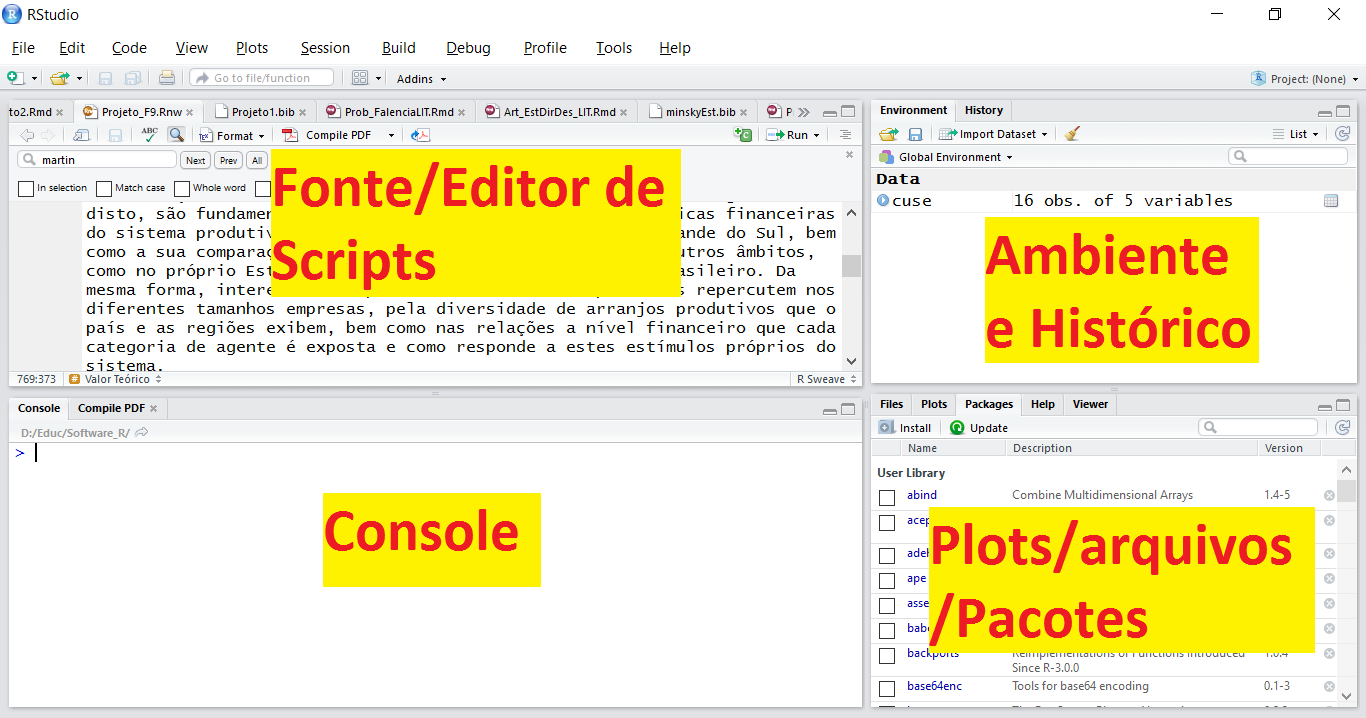
\includegraphics[width=\textwidth]{paineis} 

}

\caption{Painéis do Rstudio}\label{fig:paineis}
\end{figure}

\begin{itemize}
\tightlist
\item
  \textbf{Fonte/Editor de Scripts}: se constitui do ambiente onde serão
  abertos os scripts previamente salvos nos mais diversos formatos ou
  mesmo sendo o local de visualização das bases de dados.
\item
  \textbf{Console}: local onde será efetuada a digitação das linhas de
  código que serão interpretadas pelo R.
\item
  \textbf{Ambiente e Histórico}: o ambiente será visualizado os objetos
  criados ou carregados durante a seção e; a aba History retoma os
  scripts digitados no console.
\item
  \textbf{Plots/arquivos/Pacotes}: local onde podem ser acessados os
  arquivos salvos no computador pela aba \emph{files}; a aba
  \emph{Plots} carrega os gráficos e plotagens; a aba \emph{Packages}
  contém os pacotes instalados em seu computador, onde são ativados ou
  instalados novos; em \emph{Help} constam as ajudas e explicações dos
  pacotes e; \emph{Viewer} vizualiza documentos do tipo html.
\end{itemize}

\hypertarget{help}{%
\section{Help}\label{help}}

Acessamos a ajuda do RStudio por meio do comando \texttt{help()},
através da aba ``Help'' ou ao clicar no nome do pacote. Pode-se digitar
a ajuda que usuário necessita (exemplo \texttt{help("summary")}), ou
diretamente no colsole digitamos ? e a função desejada, exemplo:
\texttt{?mean}.

\hypertarget{instalacao-de-pacotes}{%
\section{Instalação de pacotes}\label{instalacao-de-pacotes}}

Em alguns situações, o uso de pacotes pode dar ao trabalho mais
praticidade, e para isso se faz necessário efetuar a sua instalação.
Precisamos ir até o painel dos pacotes em *packages\}, selecionar a
opção instalar e inserir o nome do pacote desejado na janela indicada.
Ao selecionar a opção instalar, no console receberemos informações do
procedimento e do sucesso do mesmo.

\begin{figure}

{\centering 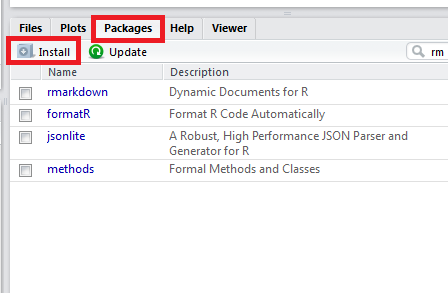
\includegraphics[width=\textwidth]{pacotes,1} 

}

\caption{Instalação de pacotes}\label{fig:pacotes1}
\end{figure}

\begin{figure}

{\centering 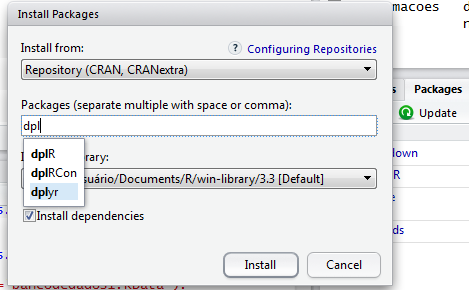
\includegraphics[width=\textwidth]{pacotes,2} 

}

\caption{Caixa de informação de pacote a ser instalado}\label{fig:pacotes2}
\end{figure}

A mesma função, para instalação de um pacote, pode ser efetuada
diretamente via console: \texttt{install.packages("pacote")}. É
importante ressaltar a função \texttt{library(nomedopacote)} que é
utilizada no console para informar ao R e ``carregar'' o pacote que o
usuário irá utilizar. Podem ser instalados mais de um pacote ao mesmo
tempo, como no exemplo:

\texttt{install.packages(c("readr",\ "readxl"))}

\hypertarget{abrir-arquivo-de-dados}{%
\section{Abrir arquivo de dados}\label{abrir-arquivo-de-dados}}

Dispondo de um banco de dados em uma planilha eletrônica (LibreOffice
Calc ou EXCEL), neste caso será utilizado o arquivo
\href{https://github.com/Smolski/softwarelivrer/raw/master/basico/arvores.xlsx}{árvores}
como exemplo o banco de dados. Os dados derivam de uma pesquisa com
espécies de árvores registrando as variáveis diâmetro altura do peito
(DAP) e altura. Dados cedidos pela professora Tatiane Chassot.

Pode-se utilizar a linha de comando para carregar os arquivos de dados,
da seguinte forma:

\texttt{library(readxl)}

\texttt{nome.objeto.xls\ =\ read\_excel("d:/arvores.xls")}

Outras opções de arquivos podem ser carregados no RStudio, como por
exemplo arquivos de texto (.txt ou .csv), arquivos derivados do excel
(.xls ou .xlsx), arquivos de dados do SPSS (.sav), do \emph{software}
SAS (.sas7bdat) e do STATA (.dta). A instalação de alguns pacotes é
requerida, dependendo da origem da base de dados, como por exemplo o
\texttt{readxl}, \texttt{readr} e \texttt{haven}, como os exemplos
abaixo:

\texttt{library(readr)}

\texttt{nomeobjeto\ =\ read.csv("d:/arvores.csv")}

\texttt{library(haven)}

\texttt{nomeobjeto\ =\ read\_sav("d:/arvores.sav")}

\texttt{nomeobjeto\ =\ read\_dta("d:/arvores.dta")}

\texttt{nomeobjeto\ =\ read\_sas("d:/arvores.sas7bdat")}

Outras opções podem ser comandadas dentro destes comando para abertura
de arquivos, como por exemplo, um arquivo csv em que esteja separado por
vírgulas pode ser lido como:

\texttt{read.csv("d:/arvores.csv",\ sep=",")}

O comando \texttt{header=TRUE} diz que a primeira linha do arquivo
contém o cabeçalho; \texttt{skip=4} faz com que sejam ignoradas as 4
primeiras linhas.

A opção \texttt{load()} (exemplo: \texttt{load("base.RData")}) pode ser
utilizada para carregar as bases de dados salvas com a função
\texttt{save()}, que será descrita no subcapítulo a seguir.

Outra opção é o carregamento das bases de dados manualmente pelo caminho
\emph{Envoirment \(>\) Import Dataset}, escolhendo o tipo de arquivo:

\begin{figure}

{\centering 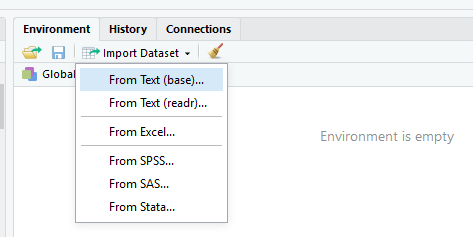
\includegraphics[width=\textwidth]{r3} 

}

\caption{Aba *Import Dataset*}\label{fig:r3}
\end{figure}

Na caixa correspondente a File/Url se insere o endereço virtual ou o
local onde se encontra o arquivo. Ao importar os dados, carrega-se um
objeto criado com as informações contidas no arquivo. No nosso exeplo,
carregamos a planilha arvores (arquivo .xls) como mostra a Figura
\ref{fig:r4}, derivado do caminho ``Import Dataset \(>\) From Excel'' do
Environment.

\begin{figure}

{\centering 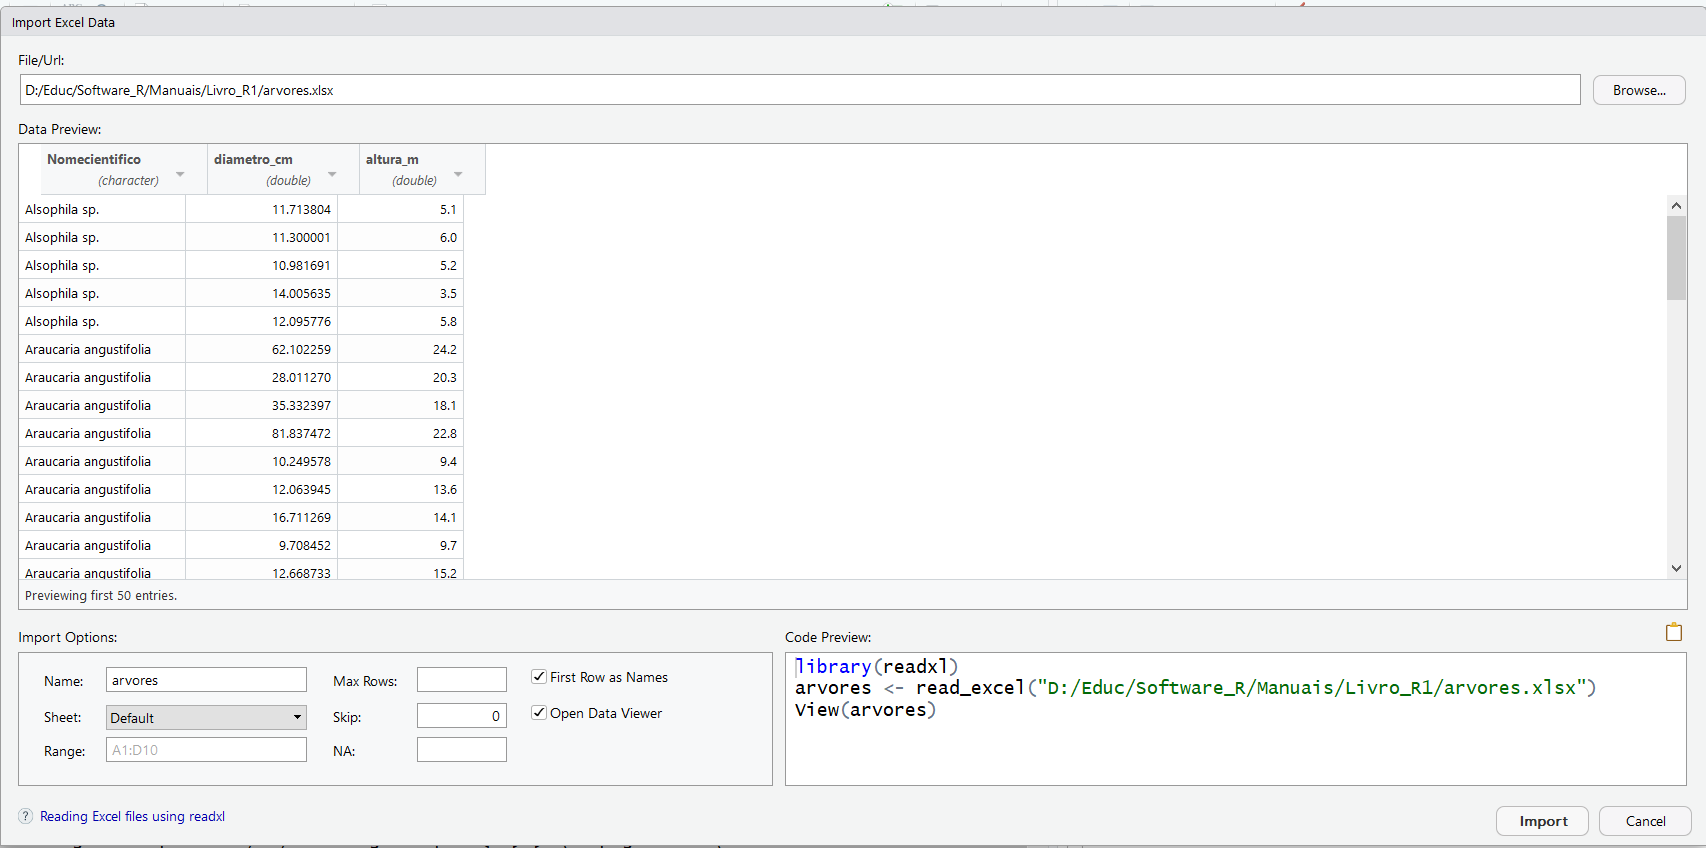
\includegraphics[width=\textwidth]{r4} 

}

\caption{Caixa de informações do Import Data}\label{fig:r4}
\end{figure}

O campo \emph{Code Preview} mostra o comando que está sendo criado para
a importação destes dados. Em \emph{Import Options}, delimita-se opções
do objeto como o nome (\emph{name}), o número máximo de linhas
(\emph{Max Rows}), quantas linhas serão puladas na importação do arquivo
(\emph{Skip}), o tratamento das células em branco (\emph{NA}) e se a
primeira linha contém os nomes (\emph{Firts Row as Names}).

Com relação à importação de arquivos de texto separado por caracteres
(.csv), ela se dá via ``Import Dataset \(>\) From Text (readr)'' do
Environment. Constam algumas solicitações diferentes a serem
determinadas pelo usuário no campo \emph{Import Options}, conforme
mostra a Figura \ref{fig:r4csv}. Uma questão importante é a opção
\emph{Delimiter}, a qual o pesquisador tem que prestar atenção quando o
arquivo está separado por vírgulas (\emph{Comma}), ponto e vírgula
(\emph{Semicolon}) ou outro tipo de caractere. A opção \emph{Locale
\(>\) Configure\ldots{}} oportuniza determinar os tipos de marca decimal
e codificação de textos, por exemplo.

\begin{figure}

{\centering 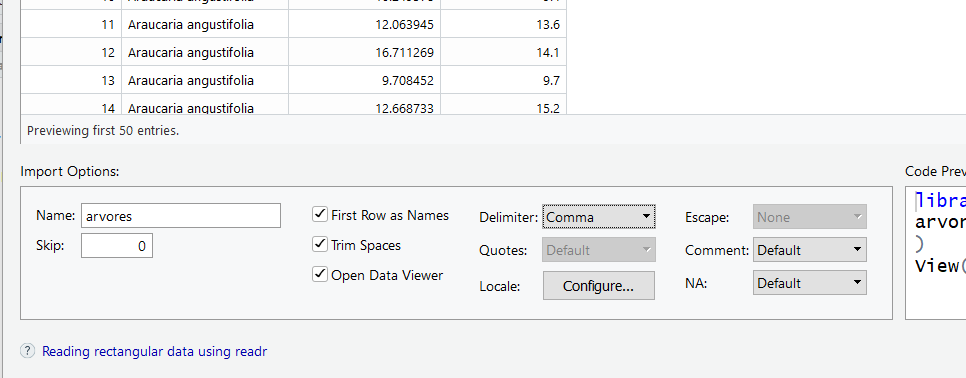
\includegraphics[width=\textwidth]{r4csv} 

}

\caption{Opções da importação de arquivos .csv}\label{fig:r4csv}
\end{figure}

Importante mencionar que em ambos os casos de importação, no campo
\emph{Dada Preview} onde constam os dados do arquivo a ser importado, é
possível determinar o tipo de dado que cada ``coluna'' contém. Isto é
extremamente importante, pois campos que possuem números, que serão
posteriormente utilizados em operações aritméticas, por exemplo, devem
ser configurados como tal. No entanto, como será visto adiante, a
alteração do tipo do dado também pode ser feita posteriormente sem
problema algum.

Alguns tipos de dados:

\begin{itemize}
\tightlist
\item
  \textbf{Numeric}: números, valores decimais em geral (\texttt{5.4}).
\item
  \textbf{Integer}: números (\texttt{4}).
\item
  \textbf{Character}: variável de texto, ou \emph{string}
  (\texttt{casa}).
\item
  \textbf{Double}: cria um vetor de precisão dupla, que abarca os
  números.
\item
  \textbf{Logical}: operadores booleanos (\texttt{TRUE,\ FALSE}).
\item
  \textbf{Date}: opção para datas.
\item
  \textbf{Time}: vetor para séries de tempo.
\item
  \textbf{Factor}: variável nominal, inclusive como fator ordenado,
  representam categorias.
\end{itemize}

\hypertarget{salvar-arquivo-de-dados}{%
\section{Salvar arquivo de dados}\label{salvar-arquivo-de-dados}}

O banco de dados que o R armazena na memória pode ser salvo, junto com
todo o ambiente, usando o ícone de disquete na aba ``Environment''
(salva como arquivo .RData), e depois carregado pelo ícone de pasta
(Abrir dados\ldots{}) na mesma aba. Desta forma, salvará todos os
objetos criados no ambiente de trabalho.

\begin{figure}

{\centering 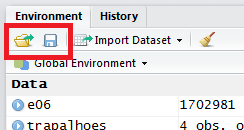
\includegraphics[width=\textwidth]{r6} 

}

\caption{Atalho para abrir e salvar arquivo de dados}\label{fig:r6}
\end{figure}

Outra opção com mesmo efeito é utilizar o comando a seguir diretamente
no console do RStudio:

\texttt{save("nomeDoObjeto",file="nomeDoArquivo.RData")}

O nome do objeto pode ser uma lista de objetos para salvar mais de um
objeto do ambiente, \texttt{list=("objeto1",\ "objeto2")}. Para carregar
um arquivo RData no ambiente, o comando a ser utilizado pelo usuário é

\texttt{load("arquivo.RData")},

desde que o arquivo esteja no diretório de trabalho do R.

É possível exportar as bases trabalhadas para vários formatos de
arquivos de dados e de texto, como seguem alguns exemplos:

\begin{itemize}
\tightlist
\item
  \texttt{write.csv(nomeobjeto,"file.csv",\ sep=";")}: salvando em
  arquivo csv.
\item
  \texttt{write.foreign(nomeobjeto,"d:/nome.sps")}: arquivos sps.
\item
  \texttt{write.foreign(nomeobjeto,"d:/nome.dta")}: arquivos dta.
\item
  \texttt{write.foreign(nomeobjeto,"d:/nome.sas7bdat")}: arquivos
  sas7bdat.
\end{itemize}

\hypertarget{diretorios-de-trabalho}{%
\section{Diretórios de trabalho}\label{diretorios-de-trabalho}}

Os trabalhos efetudados via Rstudio, incluindo as bases de dados, os
objetos, os resultados das fórmulas, os cálculos aplicados sobre os
vetores e demais arquivos resultantes da utilização do programa podem
ser salvos em seu diretório de arquivos. Após instalado o Rstudio
destina um diretório padrão salvar estes arquivos, o qual pode ser
verificado com o comando \texttt{getwd()}.

Este caminho padrão, por sua vez, pode ser alterado via comando

\texttt{setwd("C://file/path")}

onde o usuário escolhe a pasta desejada que ficará como padrão. O
comando \texttt{dir()} mostra ao usuário os documentos que constam no
diretório padrão ou o escolhido para a consulta.

\hypertarget{operacoes}{%
\section{Operações}\label{operacoes}}

\hypertarget{operacoes-aritmeticas}{%
\subsection{Operações Aritméticas}\label{operacoes-aritmeticas}}

A realização de uma operação aritmética no R acontece da seguinte forma:
onde a resolução das operações segue o padrão, ou seja, primeiro
exponenciações, seguido de multiplicações e divisões, deixando por
ultimo adições e subtrações, de acordo com a ordem que estão dispostas.
Para alterar a prioridade da resolução de operações fazemos o uso do
parenteses para destacar a operação que deve ser prioritária na
resolução. Seguem alguns exemplos efetuados diretamente no console do
RStudio:

\begin{Shaded}
\begin{Highlighting}[]
\CommentTok{# soma}
\DecValTok{19}\OperatorTok{+}\DecValTok{26}
\end{Highlighting}
\end{Shaded}

\begin{verbatim}
[1] 45
\end{verbatim}

\begin{Shaded}
\begin{Highlighting}[]
\CommentTok{# subtração}
\DecValTok{19-26}
\end{Highlighting}
\end{Shaded}

\begin{verbatim}
[1] -7
\end{verbatim}

\begin{Shaded}
\begin{Highlighting}[]
\CommentTok{# divisão}
\DecValTok{4}\OperatorTok{/}\DecValTok{2}
\end{Highlighting}
\end{Shaded}

\begin{verbatim}
[1] 2
\end{verbatim}

\begin{Shaded}
\begin{Highlighting}[]
\CommentTok{# multiplicação }
\DecValTok{4}\OperatorTok{*}\DecValTok{2}
\end{Highlighting}
\end{Shaded}

\begin{verbatim}
[1] 8
\end{verbatim}

\begin{Shaded}
\begin{Highlighting}[]
\CommentTok{# exponenciação}
\DecValTok{4}\OperatorTok{^}\DecValTok{2}
\end{Highlighting}
\end{Shaded}

\begin{verbatim}
[1] 16
\end{verbatim}

\begin{Shaded}
\begin{Highlighting}[]
\CommentTok{# prioridade de resolução}
\DecValTok{19} \OperatorTok{+}\StringTok{ }\DecValTok{26} \OperatorTok{/}\DecValTok{4} \DecValTok{-2} \OperatorTok{*}\DecValTok{10}
\end{Highlighting}
\end{Shaded}

\begin{verbatim}
[1] 5.5
\end{verbatim}

\begin{Shaded}
\begin{Highlighting}[]
\NormalTok{((}\DecValTok{19} \OperatorTok{+}\StringTok{ }\DecValTok{26}\NormalTok{) }\OperatorTok{/}\NormalTok{(}\DecValTok{4} \DecValTok{-2}\NormalTok{))}\OperatorTok{*}\DecValTok{10}
\end{Highlighting}
\end{Shaded}

\begin{verbatim}
[1] 225
\end{verbatim}

\begin{Shaded}
\begin{Highlighting}[]
\CommentTok{# raiz quadrada}
\KeywordTok{sqrt}\NormalTok{(}\DecValTok{16}\NormalTok{)}
\end{Highlighting}
\end{Shaded}

\begin{verbatim}
[1] 4
\end{verbatim}

\begin{Shaded}
\begin{Highlighting}[]
\CommentTok{# Logaritmo }
\KeywordTok{log}\NormalTok{(}\DecValTok{1}\NormalTok{)}
\end{Highlighting}
\end{Shaded}

\begin{verbatim}
[1] 0
\end{verbatim}

\hypertarget{operacoes-logicas}{%
\subsection{Operações Lógicas}\label{operacoes-logicas}}

O ambiente de programação Rstudio trabalha com algumas operações
lógicas, que serão importantes na manipulação de bases de dados:

\begin{itemize}
\tightlist
\item
  \(a == b\) (``a'' é igual a ``b'')
\item
  \(a != b\) (``a'' é diferente a ``b'')
\item
  \(a > b\) (``a'' é maior que ``b'')
\item
  \(a < b\) (``a'' é menor que ``b'')
\item
  \(a >= b\) (``a'' é maior ou igual a ``b'')
\item
  \(a <= b\) (``a'' é menor ou igual a ``b'')
\item
  is.na (``a'' é missing - faltante)
\item
  is.null (``a'' é nulo)
\end{itemize}

Seguem alguns exemplos da aplicação das operações lógicas:

\begin{Shaded}
\begin{Highlighting}[]
\CommentTok{# maior que }
\DecValTok{2} \OperatorTok{>}\StringTok{ }\DecValTok{1}
\end{Highlighting}
\end{Shaded}

\begin{verbatim}
[1] TRUE
\end{verbatim}

\begin{Shaded}
\begin{Highlighting}[]
\DecValTok{1} \OperatorTok{>}\StringTok{ }\DecValTok{2}
\end{Highlighting}
\end{Shaded}

\begin{verbatim}
[1] FALSE
\end{verbatim}

\begin{Shaded}
\begin{Highlighting}[]
\CommentTok{# menor que }
\DecValTok{1} \OperatorTok{<}\StringTok{ }\DecValTok{2}
\end{Highlighting}
\end{Shaded}

\begin{verbatim}
[1] TRUE
\end{verbatim}

\begin{Shaded}
\begin{Highlighting}[]
\CommentTok{# maior ou igual a }
\DecValTok{0} \OperatorTok{>=}\StringTok{ }\NormalTok{(}\DecValTok{2}\OperatorTok{+}\NormalTok{(}\OperatorTok{-}\DecValTok{2}\NormalTok{))}
\end{Highlighting}
\end{Shaded}

\begin{verbatim}
[1] TRUE
\end{verbatim}

\begin{Shaded}
\begin{Highlighting}[]
\CommentTok{# menor ou igual a }
\DecValTok{1} \OperatorTok{<=}\StringTok{ }\DecValTok{3}
\end{Highlighting}
\end{Shaded}

\begin{verbatim}
[1] TRUE
\end{verbatim}

\begin{Shaded}
\begin{Highlighting}[]
\CommentTok{# conjunção}
\DecValTok{9} \OperatorTok{>}\StringTok{ }\DecValTok{11} \OperatorTok{&}\StringTok{ }\DecValTok{0} \OperatorTok{<}\StringTok{ }\DecValTok{1}
\end{Highlighting}
\end{Shaded}

\begin{verbatim}
[1] FALSE
\end{verbatim}

\begin{Shaded}
\begin{Highlighting}[]
\CommentTok{# ou}
\DecValTok{6} \OperatorTok{<}\StringTok{ }\DecValTok{5} \OperatorTok{|}\StringTok{ }\DecValTok{0} \OperatorTok{>}\StringTok{ }\DecValTok{-1}
\end{Highlighting}
\end{Shaded}

\begin{verbatim}
[1] TRUE
\end{verbatim}

\begin{Shaded}
\begin{Highlighting}[]
\CommentTok{# igual a}
\DecValTok{1} \OperatorTok{==}\StringTok{ }\DecValTok{2}\OperatorTok{/}\DecValTok{2}
\end{Highlighting}
\end{Shaded}

\begin{verbatim}
[1] TRUE
\end{verbatim}

\begin{Shaded}
\begin{Highlighting}[]
\CommentTok{# diferente de}
\DecValTok{1} \OperatorTok{!=}\StringTok{ }\DecValTok{2}
\end{Highlighting}
\end{Shaded}

\begin{verbatim}
[1] TRUE
\end{verbatim}

\hypertarget{criacao-de-variaveis}{%
\section{Criação de variáveis}\label{criacao-de-variaveis}}

A linguagem de programação R se configura em uma linguagem orientada a
objetos, ou seja, a todo tempo estamos criando diversos tipos de objetos
e efetuando operações com os mesmos. Por exemplo, a criação de listas,
bases de dados, união de bases de dados, data.frames e até mesmo mapas!

\begin{Shaded}
\begin{Highlighting}[]
\CommentTok{#Criando um objeto simples}
\NormalTok{objeto =}\StringTok{ "meu primeiro objeto"} \CommentTok{#enter}
\CommentTok{#Agora para retomar o objeto criado:}
\NormalTok{objeto }\CommentTok{#enter}
\end{Highlighting}
\end{Shaded}

\begin{verbatim}
[1] "meu primeiro objeto"
\end{verbatim}

\begin{Shaded}
\begin{Highlighting}[]
\CommentTok{#Pode ser efetuada uma operação:}
\NormalTok{a=}\StringTok{ }\DecValTok{2}\OperatorTok{+}\DecValTok{1}
\NormalTok{a}
\end{Highlighting}
\end{Shaded}

\begin{verbatim}
[1] 3
\end{verbatim}

O comando \texttt{ls()} lista todos os objetos que estão criados no
ambiente e \texttt{rm(x)} remove o objeto indicado (x). Para remover
todos os objetos de uma só vez utiliza-se \texttt{rm(list=ls())}.

\begin{Shaded}
\begin{Highlighting}[]
\CommentTok{#Lista objetos do ambiente}
\KeywordTok{ls}\NormalTok{()}
\end{Highlighting}
\end{Shaded}

\begin{verbatim}
[1] "a"      "objeto"
\end{verbatim}

\begin{Shaded}
\begin{Highlighting}[]
\CommentTok{#Remover um banco de dados}
\KeywordTok{rm}\NormalTok{(a)}
\end{Highlighting}
\end{Shaded}

\hypertarget{conversao-de-uma-variavel}{%
\subsection{Conversão de uma variável}\label{conversao-de-uma-variavel}}

Para a aplicação de algumas funções é importante que cada variável
esteja corretamente classificada, o que em alguns casos não ocorre
durante o reconhecimento automático do R. Precisamos então reconhecê-la
como variável texto, numérica ou fator. Além disso, a classe ordered se
aplica a variáveis categóricas que podem ser consideradas ordenáveis.

\begin{Shaded}
\begin{Highlighting}[]
\NormalTok{idade=}\KeywordTok{c}\NormalTok{(}\StringTok{'11'}\NormalTok{, }\StringTok{'12'}\NormalTok{, }\StringTok{'31'}\NormalTok{)}
\NormalTok{nomes=}\KeywordTok{c}\NormalTok{(}\StringTok{"Elisa"}\NormalTok{, }\StringTok{"Priscila"}\NormalTok{, }\StringTok{"Carol"}\NormalTok{)}
\NormalTok{cep=}\KeywordTok{c}\NormalTok{(}\DecValTok{98700000}\NormalTok{,}\DecValTok{98701000}\NormalTok{,}\DecValTok{98702000}\NormalTok{)}
\NormalTok{idade=}\StringTok{ }\KeywordTok{as.numeric}\NormalTok{(idade)}
\NormalTok{idade}
\end{Highlighting}
\end{Shaded}

\begin{verbatim}
[1] 11 12 31
\end{verbatim}

\begin{Shaded}
\begin{Highlighting}[]
\NormalTok{cep =}\StringTok{ }\KeywordTok{as.character}\NormalTok{(cep)}
\NormalTok{cep}
\end{Highlighting}
\end{Shaded}

\begin{verbatim}
[1] "98700000" "98701000" "98702000"
\end{verbatim}

\hypertarget{alguns-comandos-essenciais}{%
\section{Alguns comandos essenciais}\label{alguns-comandos-essenciais}}

A função \texttt{head()} mostra as 6 primeiras colunas do arquivo para
se ter uma noção do conteúdo. No caso do mesmo ser um data.frame,
podemos solicitar o número de valores ou linhas a serem mostrados no
console através do parâmetro n ou na ausência deste, todas as linhas
serão impressas, como exemplo \texttt{head(x\ ,n=2)} para ver as duas
primeiras linhas.

O comando \texttt{summary()} efetua o resumo dos dados, se for
qualitativa mostra a frequência absoluta das categorias e se for
quantitativa apresenta as categorias. No exemplo abaixo trabalharemos
com uma base de dados de treinamento denominada ``iris'' que está
acessível no \emph{software} RStudio através do comando que carrega
dados específicos \texttt{data()}:

\begin{Shaded}
\begin{Highlighting}[]
\CommentTok{#Carregando dados da base do RSdudio iris.}
\KeywordTok{data}\NormalTok{(iris)}

\CommentTok{#Visualizando as primeiras 6 colunas}
\KeywordTok{head}\NormalTok{(iris)}
\end{Highlighting}
\end{Shaded}

\begin{verbatim}
  Sepal.Length Sepal.Width Petal.Length Petal.Width Species
1          5.1         3.5          1.4         0.2  setosa
2          4.9         3.0          1.4         0.2  setosa
3          4.7         3.2          1.3         0.2  setosa
4          4.6         3.1          1.5         0.2  setosa
5          5.0         3.6          1.4         0.2  setosa
6          5.4         3.9          1.7         0.4  setosa
\end{verbatim}

\begin{Shaded}
\begin{Highlighting}[]
\CommentTok{#Resumo do objeto}
\KeywordTok{summary}\NormalTok{(iris)}
\end{Highlighting}
\end{Shaded}

\begin{verbatim}
  Sepal.Length   Sepal.Width    Petal.Length   Petal.Width        Species  
 Min.   :4.30   Min.   :2.00   Min.   :1.00   Min.   :0.1   setosa    :50  
 1st Qu.:5.10   1st Qu.:2.80   1st Qu.:1.60   1st Qu.:0.3   versicolor:50  
 Median :5.80   Median :3.00   Median :4.35   Median :1.3   virginica :50  
 Mean   :5.84   Mean   :3.06   Mean   :3.76   Mean   :1.2                  
 3rd Qu.:6.40   3rd Qu.:3.30   3rd Qu.:5.10   3rd Qu.:1.8                  
 Max.   :7.90   Max.   :4.40   Max.   :6.90   Max.   :2.5                  
\end{verbatim}

O comando \texttt{names()} lista os nomes das colunas dos bancos de
dados escolhidos, enquanto \texttt{tail()} mostra as últimas seis
linhas.

\begin{Shaded}
\begin{Highlighting}[]
\CommentTok{#Para visualizar os nomes das colunas dos dados:}
\KeywordTok{names}\NormalTok{(iris)}
\end{Highlighting}
\end{Shaded}

\begin{verbatim}
[1] "Sepal.Length" "Sepal.Width"  "Petal.Length" "Petal.Width"  "Species"     
\end{verbatim}

\begin{Shaded}
\begin{Highlighting}[]
\CommentTok{#vizualizar as ultimas seis linhas do objetos}
\KeywordTok{tail}\NormalTok{(iris)}
\end{Highlighting}
\end{Shaded}

\begin{verbatim}
    Sepal.Length Sepal.Width Petal.Length Petal.Width   Species
145          6.7         3.3          5.7         2.5 virginica
146          6.7         3.0          5.2         2.3 virginica
147          6.3         2.5          5.0         1.9 virginica
148          6.5         3.0          5.2         2.0 virginica
149          6.2         3.4          5.4         2.3 virginica
150          5.9         3.0          5.1         1.8 virginica
\end{verbatim}

Para que o pesquisador conheça melhor as bases de dados em que está
atuando, o comando \texttt{class()} serve para identificar o tipo de
base ou dados da base. Com o exemplo abaixo constata-se que o objeto
``iris'' é um \emph{data frame}, a variável ``Sepal.Length'' é uma
variável numérica e que a variável numérica.

\begin{Shaded}
\begin{Highlighting}[]
\KeywordTok{class}\NormalTok{(iris)}
\end{Highlighting}
\end{Shaded}

\begin{verbatim}
[1] "data.frame"
\end{verbatim}

\begin{Shaded}
\begin{Highlighting}[]
\KeywordTok{class}\NormalTok{(iris}\OperatorTok{$}\NormalTok{Sepal.Length)}
\end{Highlighting}
\end{Shaded}

\begin{verbatim}
[1] "numeric"
\end{verbatim}

\begin{Shaded}
\begin{Highlighting}[]
\KeywordTok{class}\NormalTok{(iris}\OperatorTok{$}\NormalTok{Especie)}
\end{Highlighting}
\end{Shaded}

\begin{verbatim}
[1] "NULL"
\end{verbatim}

Efeito semelhante possui o comando \texttt{ls.str()}:

\begin{Shaded}
\begin{Highlighting}[]
\KeywordTok{ls.str}\NormalTok{(iris)}
\end{Highlighting}
\end{Shaded}

\begin{verbatim}
Petal.Length :  num [1:150] 1.4 1.4 1.3 1.5 1.4 1.7 1.4 1.5 1.4 1.5 ...
Petal.Width :  num [1:150] 0.2 0.2 0.2 0.2 0.2 0.4 0.3 0.2 0.2 0.1 ...
Sepal.Length :  num [1:150] 5.1 4.9 4.7 4.6 5 5.4 4.6 5 4.4 4.9 ...
Sepal.Width :  num [1:150] 3.5 3 3.2 3.1 3.6 3.9 3.4 3.4 2.9 3.1 ...
Species :  Factor w/ 3 levels "setosa","versicolor",..: 1 1 1 1 1 1 1 1 1 1 ...
\end{verbatim}

Os comandos \texttt{ncol()} e \texttt{nrow()} mostram o número de
colunas e o número de linhas do objeto, respectivamente.

\hypertarget{funcoes-view-e-dim}{%
\subsection{\texorpdfstring{Funções \emph{View} e
\emph{dim}}{Funções View e dim}}\label{funcoes-view-e-dim}}

A função \texttt{View()} permite vizualizar os elementos no script do
dataframe requesitado, enquando a função \texttt{dim()} (abreviatura de
dimensões) fornece o número de linhas e de colunas, respectivamente.

\begin{Shaded}
\begin{Highlighting}[]
\KeywordTok{View}\NormalTok{(iris)}
\KeywordTok{dim}\NormalTok{(iris)}
\end{Highlighting}
\end{Shaded}

\begin{verbatim}
[1] 150   5
\end{verbatim}

Para alterar um nome de uma variável pode ser utilizado o comando
colnames. No exemplo acima, vamos alterar o nome da coluna ``Species''
para ``Especie''.

\begin{Shaded}
\begin{Highlighting}[]
\CommentTok{#Alterar o nome da coluna, sendo que o '[5]' indica que está na quinta coluna.}
\KeywordTok{colnames}\NormalTok{(iris)[}\DecValTok{5}\NormalTok{]=}\StringTok{'Especie'}
\end{Highlighting}
\end{Shaded}

Para selecionarmos uma coluna do objeto ``iris'', por exemplo a coluna
``Sepal.Length'', poderíamos digitar no console o comando
\textbf{iris\$Sepal.Length}. O padrão de carregamento da base de dados
nos obriga a dizer ao R qual é a base que quer selecionar (iris),
inserindo o símbolo \texttt{\$} e após o nome da coluna a qual deseja as
informações. Para criar um novo objeto com esta informação, basta dizer
ao R, como já visto acima, por exemplo:
\textbf{novoobjeto=iris\$novacoluna}.

No entanto, para acessar os dados sem o uso do símbolo \texttt{\$},
podemos usar o seguinte comando: \textbf{attach(iris)}. Assim, podemos
efetuar o sumário da coluna ``Petal.Width'':

\begin{Shaded}
\begin{Highlighting}[]
\CommentTok{#Definindo a função attach para o objeto 'dados'.}
\KeywordTok{attach}\NormalTok{(iris)}
\CommentTok{#Efetuando o sumário de 'pop.total'.}
\KeywordTok{summary}\NormalTok{(Petal.Width)}
\end{Highlighting}
\end{Shaded}

\begin{verbatim}
   Min. 1st Qu.  Median    Mean 3rd Qu.    Max. 
    0.1     0.3     1.3     1.2     1.8     2.5 
\end{verbatim}

\begin{Shaded}
\begin{Highlighting}[]
\CommentTok{#Como a coluna 'distrito' é um fator, o sumário será }
\CommentTok{#a contagem da quantidade de cada fator na coluna.}
\KeywordTok{summary}\NormalTok{(Especie)}
\end{Highlighting}
\end{Shaded}

\begin{verbatim}
    setosa versicolor  virginica 
        50         50         50 
\end{verbatim}

\hypertarget{comando-tapply}{%
\subsection{\texorpdfstring{Comando
\emph{tapply}}{Comando tapply}}\label{comando-tapply}}

O comando \texttt{taply()} agrega os dados pelos níveis das variáveis
qualitativas. Note que a coluna ``Especie'' possui dados em forma de
fatores. Assim, para filtrarmos a informação (coluna ``Sepal.Length'')
média por Especie, podemos utilizar:

\begin{Shaded}
\begin{Highlighting}[]
\CommentTok{#Função 'tapply', número médio da população total por distrito.}
\KeywordTok{tapply}\NormalTok{(Sepal.Length, Especie, mean)}
\end{Highlighting}
\end{Shaded}

\begin{verbatim}
    setosa versicolor  virginica 
     5.006      5.936      6.588 
\end{verbatim}

No caso da coluna ``Sepal.Length'', se ela possuir um registro NA
(faltante), para que se efetue a média por este coluna neste quesito, há
que se adicionar o parâmetro \texttt{na.rm=T}, que ignora as células
faltantes para calcular-se a média:

\begin{Shaded}
\begin{Highlighting}[]
\CommentTok{#Função 'tapply' considerando NAs:}
\KeywordTok{tapply}\NormalTok{(Sepal.Length, Especie, mean)}
\end{Highlighting}
\end{Shaded}

\begin{verbatim}
    setosa versicolor  virginica 
     5.006      5.936      6.588 
\end{verbatim}

\begin{Shaded}
\begin{Highlighting}[]
\CommentTok{#Função 'tapply' sem considerar NAs:}
\KeywordTok{tapply}\NormalTok{(Sepal.Length, Especie, mean, }\DataTypeTok{na.rm=}\NormalTok{T)}
\end{Highlighting}
\end{Shaded}

\begin{verbatim}
    setosa versicolor  virginica 
     5.006      5.936      6.588 
\end{verbatim}

\hypertarget{comando-subset}{%
\subsection{\texorpdfstring{Comando
\emph{subset}}{Comando subset}}\label{comando-subset}}

Utiliza-se o comando \texttt{subset()} para formar um subconjunto de
dados o qual desejamos selecionar de um objeto. Por exemplo, se
quisermos criar um novo objeto com somente os dados da ``Especie''
setosa:

\begin{Shaded}
\begin{Highlighting}[]
\NormalTok{dadossetosa=}\KeywordTok{subset}\NormalTok{(iris, Especie}\OperatorTok{==}\StringTok{'setosa'}\NormalTok{)}
\KeywordTok{head}\NormalTok{(dadossetosa)}
\end{Highlighting}
\end{Shaded}

\begin{verbatim}
  Sepal.Length Sepal.Width Petal.Length Petal.Width Especie
1          5.1         3.5          1.4         0.2  setosa
2          4.9         3.0          1.4         0.2  setosa
3          4.7         3.2          1.3         0.2  setosa
4          4.6         3.1          1.5         0.2  setosa
5          5.0         3.6          1.4         0.2  setosa
6          5.4         3.9          1.7         0.4  setosa
\end{verbatim}

Pode ser configurado mais de uma condição para a filtragem dos dados,
por exemplo, além de serem filtrados os dados referentes a Especie
setosa, aquelas na qual o Sepal.Length é superior a 5. Como no exemplo,
criamos um novo objeto com estas condições:

\begin{Shaded}
\begin{Highlighting}[]
\NormalTok{dadossetosa2=}\KeywordTok{subset}\NormalTok{(iris, Especie}\OperatorTok{==}\StringTok{'setosa'}\OperatorTok{&}\StringTok{ }\NormalTok{Sepal.Length}\OperatorTok{>}\DecValTok{5}\NormalTok{)}
\KeywordTok{head}\NormalTok{(dadossetosa2)}
\end{Highlighting}
\end{Shaded}

\begin{verbatim}
   Sepal.Length Sepal.Width Petal.Length Petal.Width Especie
1           5.1         3.5          1.4         0.2  setosa
6           5.4         3.9          1.7         0.4  setosa
11          5.4         3.7          1.5         0.2  setosa
15          5.8         4.0          1.2         0.2  setosa
16          5.7         4.4          1.5         0.4  setosa
17          5.4         3.9          1.3         0.4  setosa
\end{verbatim}

\hypertarget{estrutura-de-dados}{%
\section{Estrutura de dados}\label{estrutura-de-dados}}

\hypertarget{vetores}{%
\subsection{Vetores}\label{vetores}}

Os fatores são uma classe especial de vetores, que definem variáveis
categóricas de classificação, como os tratamentos em um experimento
fatorial, ou categorias em uma tabela de contingência.

\begin{Shaded}
\begin{Highlighting}[]
\CommentTok{# Criação de um vetor}
\NormalTok{x=}\StringTok{ }\KeywordTok{c}\NormalTok{(}\DecValTok{2}\NormalTok{, }\DecValTok{4}\NormalTok{, }\DecValTok{6}\NormalTok{)}
\NormalTok{x}
\end{Highlighting}
\end{Shaded}

\begin{verbatim}
[1] 2 4 6
\end{verbatim}

Os vetores podem ser criados a partir de uma sequência numérica ou mesmo
de um intervalo entre valores:

\begin{Shaded}
\begin{Highlighting}[]
\NormalTok{x=}\StringTok{ }\KeywordTok{c}\NormalTok{(}\DecValTok{2}\OperatorTok{:}\DecValTok{6}\NormalTok{)}
\NormalTok{x}
\end{Highlighting}
\end{Shaded}

\begin{verbatim}
[1] 2 3 4 5 6
\end{verbatim}

\begin{Shaded}
\begin{Highlighting}[]
\CommentTok{# Criação de um vetor a partir do intervalo entre cada elemento e valores}
\CommentTok{#mínimo e máximo}
\NormalTok{x=}\StringTok{ }\KeywordTok{seq}\NormalTok{(}\DecValTok{2}\NormalTok{, }\DecValTok{3}\NormalTok{, }\DataTypeTok{by=}\FloatTok{0.5}\NormalTok{)}
\NormalTok{x}
\end{Highlighting}
\end{Shaded}

\begin{verbatim}
[1] 2.0 2.5 3.0
\end{verbatim}

Criação de um vetor atráves de uma repetição também é útil em várias
situações. No primeiro exemplo repete o intervalo de 1 a 3 4 vezes e no
segundo exemplo, a cada 3 vezes:

\begin{Shaded}
\begin{Highlighting}[]
\NormalTok{x=}\StringTok{ }\KeywordTok{rep}\NormalTok{(}\DecValTok{1}\OperatorTok{:}\DecValTok{3}\NormalTok{, }\DataTypeTok{times=}\DecValTok{4}\NormalTok{)}
\NormalTok{x}
\end{Highlighting}
\end{Shaded}

\begin{verbatim}
 [1] 1 2 3 1 2 3 1 2 3 1 2 3
\end{verbatim}

\begin{Shaded}
\begin{Highlighting}[]
\NormalTok{y=}\StringTok{ }\KeywordTok{rep}\NormalTok{(}\DecValTok{1}\OperatorTok{:}\DecValTok{3}\NormalTok{, }\DataTypeTok{each=}\DecValTok{3}\NormalTok{)}
\NormalTok{y}
\end{Highlighting}
\end{Shaded}

\begin{verbatim}
[1] 1 1 1 2 2 2 3 3 3
\end{verbatim}

A função factor cria um fator, a partir de um vetor:

\begin{Shaded}
\begin{Highlighting}[]
\NormalTok{sexo<-}\KeywordTok{factor}\NormalTok{(}\KeywordTok{rep}\NormalTok{(}\KeywordTok{c}\NormalTok{(}\StringTok{"F"}\NormalTok{, }\StringTok{"M"}\NormalTok{),}\DataTypeTok{each=}\DecValTok{8}\NormalTok{))}
\NormalTok{sexo}
\end{Highlighting}
\end{Shaded}

\begin{verbatim}
 [1] F F F F F F F F M M M M M M M M
Levels: F M
\end{verbatim}

\begin{Shaded}
\begin{Highlighting}[]
\NormalTok{numeros=}\KeywordTok{rep}\NormalTok{(}\DecValTok{1}\OperatorTok{:}\DecValTok{3}\NormalTok{,}\DataTypeTok{each=}\DecValTok{3}\NormalTok{)}
\NormalTok{numeros}
\end{Highlighting}
\end{Shaded}

\begin{verbatim}
[1] 1 1 1 2 2 2 3 3 3
\end{verbatim}

\begin{Shaded}
\begin{Highlighting}[]
\NormalTok{numeros.f<-}\KeywordTok{factor}\NormalTok{(numeros)}
\NormalTok{numeros.f}
\end{Highlighting}
\end{Shaded}

\begin{verbatim}
[1] 1 1 1 2 2 2 3 3 3
Levels: 1 2 3
\end{verbatim}

Fatores têm um atributo que especifica seus níveis ou categorias
(levels), que seguem ordem alfanumérica crescente, por \emph{default}.
Em muitas análises essa ordem é de fundamental importância e dessa forma
pode ser alterada através do argumento levels, por exemplo, para que
possa ser colocado o controle antes dos tratamentos:

\begin{Shaded}
\begin{Highlighting}[]
\NormalTok{tratamentos=}\KeywordTok{factor}\NormalTok{(}\KeywordTok{rep}\NormalTok{(}\KeywordTok{c}\NormalTok{(}\StringTok{"controle"}\NormalTok{,}\StringTok{"adubo A"}\NormalTok{,}\StringTok{"adubo B"}\NormalTok{), }\DataTypeTok{each=}\DecValTok{4}\NormalTok{))}
\NormalTok{tratamentos}
\end{Highlighting}
\end{Shaded}

\begin{verbatim}
 [1] controle controle controle controle adubo A  adubo A  adubo A  adubo A 
 [9] adubo B  adubo B  adubo B  adubo B 
Levels: adubo A adubo B controle
\end{verbatim}

\begin{Shaded}
\begin{Highlighting}[]
\NormalTok{tratamentos=}\KeywordTok{factor}\NormalTok{(}\KeywordTok{rep}\NormalTok{(}\KeywordTok{c}\NormalTok{(}\StringTok{"controle"}\NormalTok{,}\StringTok{"adubo A"}\NormalTok{,}\StringTok{"adubo B"}\NormalTok{), }\DataTypeTok{each=}\DecValTok{4}\NormalTok{), }
\DataTypeTok{levels=}\KeywordTok{c}\NormalTok{(}\StringTok{"controle"}\NormalTok{, }\StringTok{"adubo A"}\NormalTok{, }\StringTok{"adubo B"}\NormalTok{))}
\NormalTok{tratamentos}
\end{Highlighting}
\end{Shaded}

\begin{verbatim}
 [1] controle controle controle controle adubo A  adubo A  adubo A  adubo A 
 [9] adubo B  adubo B  adubo B  adubo B 
Levels: controle adubo A adubo B
\end{verbatim}

Fatores podem conter níveis não usados (vazios):

\begin{Shaded}
\begin{Highlighting}[]
\NormalTok{participantes=}\KeywordTok{factor}\NormalTok{(}\KeywordTok{rep}\NormalTok{(}\StringTok{"mulheres"}\NormalTok{,}\DecValTok{10}\NormalTok{), }\DataTypeTok{levels=}\KeywordTok{c}\NormalTok{(}\StringTok{"mulheres"}\NormalTok{,}\StringTok{"homens"}\NormalTok{))}
\NormalTok{participantes}
\end{Highlighting}
\end{Shaded}

\begin{verbatim}
 [1] mulheres mulheres mulheres mulheres mulheres mulheres mulheres mulheres
 [9] mulheres mulheres
Levels: mulheres homens
\end{verbatim}

Também é possível aplicar uma função aos subconjuntos de um vetor
definidos por um fator utilizando a função \texttt{tapply()}. Criamos um
objeto com o sexo das pessoas, seguido pela dieta e peso (que
caracterizamos como numérico). Depois, determinamos a média de peso
frente ao sexo e a dieta

\begin{Shaded}
\begin{Highlighting}[]
\NormalTok{sexo=}\KeywordTok{factor}\NormalTok{(}\KeywordTok{rep}\NormalTok{(}\KeywordTok{c}\NormalTok{(}\StringTok{"F"}\NormalTok{,}\StringTok{"M"}\NormalTok{),}\DataTypeTok{each=}\DecValTok{9}\NormalTok{))}
\NormalTok{dieta=}\KeywordTok{factor}\NormalTok{(}\KeywordTok{rep}\NormalTok{(}\KeywordTok{rep}\NormalTok{(}\KeywordTok{c}\NormalTok{(}\StringTok{"normal"}\NormalTok{,}\StringTok{"light"}\NormalTok{,}\StringTok{"diet"}\NormalTok{), }\DataTypeTok{each=}\DecValTok{3}\NormalTok{),}\DecValTok{2}\NormalTok{), }
\DataTypeTok{levels=}\KeywordTok{c}\NormalTok{(}\StringTok{"normal"}\NormalTok{, }\StringTok{"light"}\NormalTok{,}\StringTok{"diet"}\NormalTok{))}
\NormalTok{peso=}\KeywordTok{c}\NormalTok{(}\DecValTok{90}\NormalTok{, }\DecValTok{89}\NormalTok{, }\DecValTok{78}\NormalTok{, }\DecValTok{69}\NormalTok{, }\DecValTok{85}\NormalTok{, }\DecValTok{69}\NormalTok{, }\DecValTok{77}\NormalTok{, }\DecValTok{89}\NormalTok{, }\DecValTok{80}\NormalTok{, }\DecValTok{60}\NormalTok{, }\DecValTok{75}\NormalTok{, }\DecValTok{79}\NormalTok{, }\DecValTok{65}\NormalTok{, }\DecValTok{94}\NormalTok{,}
       \DecValTok{69}\NormalTok{, }\DecValTok{85}\NormalTok{, }\DecValTok{69}\NormalTok{, }\DecValTok{77}\NormalTok{)}
\NormalTok{sexo}
\end{Highlighting}
\end{Shaded}

\begin{verbatim}
 [1] F F F F F F F F F M M M M M M M M M
Levels: F M
\end{verbatim}

\begin{Shaded}
\begin{Highlighting}[]
\NormalTok{dieta}
\end{Highlighting}
\end{Shaded}

\begin{verbatim}
 [1] normal normal normal light  light  light  diet   diet   diet   normal
[11] normal normal light  light  light  diet   diet   diet  
Levels: normal light diet
\end{verbatim}

\begin{Shaded}
\begin{Highlighting}[]
\NormalTok{peso=}\KeywordTok{as.numeric}\NormalTok{(peso)}

\CommentTok{# média de peso frente ao sexo e dieta}
\KeywordTok{tapply}\NormalTok{(peso,}\KeywordTok{list}\NormalTok{(sexo,dieta), mean)}
\end{Highlighting}
\end{Shaded}

\begin{verbatim}
  normal light diet
F  85.67 74.33   82
M  71.33 76.00   77
\end{verbatim}

\hypertarget{funcao-table}{%
\subsubsection{\texorpdfstring{Função
\emph{table}}{Função table}}\label{funcao-table}}

Para contar elementos em cada nível de um fator, usa-se a função table:

\begin{Shaded}
\begin{Highlighting}[]
\KeywordTok{table}\NormalTok{(participantes)}
\end{Highlighting}
\end{Shaded}

\begin{verbatim}
participantes
mulheres   homens 
      10        0 
\end{verbatim}

A função pode fazer tabulações cruzadas, gerando uma tabela de
contingência, esse tipo de tabela é usado para registrar observações
independentes de duas ou mais variáveis aleatórias:

\begin{Shaded}
\begin{Highlighting}[]
\KeywordTok{table}\NormalTok{(sexo,dieta)}
\end{Highlighting}
\end{Shaded}

\begin{verbatim}
    dieta
sexo normal light diet
   F      3     3    3
   M      3     3    3
\end{verbatim}

\hypertarget{matrizes}{%
\subsection{Matrizes}\label{matrizes}}

A função matrix tem a finalidade de criar uma matriz com os valores do
argumento data, argumento este que insere as variáveis desejadas na
matriz. O número de linhas é definido pelo argumento nrow e o número de
colunas é definido pelo argumento ncol:

\begin{Shaded}
\begin{Highlighting}[]
\NormalTok{nome.da.matriz=}\StringTok{ }\KeywordTok{matrix}\NormalTok{(}\DataTypeTok{data=}\DecValTok{1}\OperatorTok{:}\DecValTok{12}\NormalTok{,}\DataTypeTok{nrow =} \DecValTok{3}\NormalTok{,}\DataTypeTok{ncol =} \DecValTok{4}\NormalTok{)}
\NormalTok{nome.da.matriz}
\end{Highlighting}
\end{Shaded}

\begin{verbatim}
     [,1] [,2] [,3] [,4]
[1,]    1    4    7   10
[2,]    2    5    8   11
[3,]    3    6    9   12
\end{verbatim}

Por \emph{default} (ação tomada pelo \emph{software}), os valores são
preenchidos por coluna. Para preencher por linha basta instruir o
programa de outra forma, alterando o argumento \texttt{byrow} para TRUE:

\begin{Shaded}
\begin{Highlighting}[]
\NormalTok{nome.da.matriz=}\StringTok{ }\KeywordTok{matrix}\NormalTok{(}\DataTypeTok{data=}\DecValTok{1}\OperatorTok{:}\DecValTok{12}\NormalTok{,}\DataTypeTok{nrow =} \DecValTok{3}\NormalTok{,}\DataTypeTok{ncol =} \DecValTok{4}\NormalTok{, }\DataTypeTok{byrow=}\NormalTok{T)}
\NormalTok{nome.da.matriz}
\end{Highlighting}
\end{Shaded}

\begin{verbatim}
     [,1] [,2] [,3] [,4]
[1,]    1    2    3    4
[2,]    5    6    7    8
[3,]    9   10   11   12
\end{verbatim}

Se a matriz inserida tem menos elementos do que a ordem informada para a
matriz, os são repetidos até preenchê-la:

\begin{Shaded}
\begin{Highlighting}[]
\NormalTok{lista=}\StringTok{ }\KeywordTok{list}\NormalTok{(}\DataTypeTok{matriz=}\KeywordTok{matrix}\NormalTok{(}\KeywordTok{c}\NormalTok{(}\DecValTok{1}\NormalTok{,}\DecValTok{2}\NormalTok{,}\DecValTok{1}\NormalTok{), }\DataTypeTok{nrow=}\DecValTok{3}\NormalTok{, }\DataTypeTok{ncol=}\DecValTok{2}\NormalTok{))}
\NormalTok{lista}
\end{Highlighting}
\end{Shaded}

\begin{verbatim}
$matriz
     [,1] [,2]
[1,]    1    1
[2,]    2    2
[3,]    1    1
\end{verbatim}

\hypertarget{listas}{%
\subsection{Listas}\label{listas}}

As listas podem ser criadas a partir do comando \texttt{list()}.

\begin{itemize}
\tightlist
\item
  \textbf{nrow}: corresponde ao número de linhas;
\item
  \textbf{ncol}: corresponde ao número de colunas.
\end{itemize}

Para ver quais elementos estão em suas listas é só chamar pelo nome que
foi dado para ela, como no exemplo abaixo. Representa uma coleção de
objetos.

\begin{Shaded}
\begin{Highlighting}[]
\NormalTok{lista=}\StringTok{ }\KeywordTok{list}\NormalTok{(}\DataTypeTok{matriz=}\KeywordTok{matrix}\NormalTok{(}\KeywordTok{c}\NormalTok{(}\DecValTok{1}\NormalTok{,}\DecValTok{2}\NormalTok{,}\DecValTok{1}\NormalTok{,}\DecValTok{5}\NormalTok{,}\DecValTok{7}\NormalTok{,}\DecValTok{9}\NormalTok{), }\DataTypeTok{nrow=}\DecValTok{3}\NormalTok{, }\DataTypeTok{ncol=}\DecValTok{2}\NormalTok{),}\DataTypeTok{vetor=}\DecValTok{1}\OperatorTok{:}\DecValTok{6}\NormalTok{)}
\NormalTok{lista}
\end{Highlighting}
\end{Shaded}

\begin{verbatim}
$matriz
     [,1] [,2]
[1,]    1    5
[2,]    2    7
[3,]    1    9

$vetor
[1] 1 2 3 4 5 6
\end{verbatim}

\hypertarget{comandos-para-manipulacao-de-listas}{%
\subsubsection{Comandos para manipulação de
listas}\label{comandos-para-manipulacao-de-listas}}

Para descobrirmos de maneira rápida o números de objetos que há na
lista, utilizamos o comando \texttt{length(nomedalista)}.

\begin{Shaded}
\begin{Highlighting}[]
\NormalTok{lista}
\end{Highlighting}
\end{Shaded}

\begin{verbatim}
$matriz
     [,1] [,2]
[1,]    1    5
[2,]    2    7
[3,]    1    9

$vetor
[1] 1 2 3 4 5 6
\end{verbatim}

\begin{Shaded}
\begin{Highlighting}[]
\KeywordTok{length}\NormalTok{(lista)}
\end{Highlighting}
\end{Shaded}

\begin{verbatim}
[1] 2
\end{verbatim}

O uso do comando \texttt{names(nomedalista)} retorna os nomes dos
objetos que estão presentes na lista.

\begin{Shaded}
\begin{Highlighting}[]
\KeywordTok{names}\NormalTok{(lista)}
\end{Highlighting}
\end{Shaded}

\begin{verbatim}
[1] "matriz" "vetor" 
\end{verbatim}

Para chamar várias listas através usamos o comando da seguinte forma:

\texttt{c(nome1,\ nome2)}

\begin{Shaded}
\begin{Highlighting}[]
\NormalTok{lista}\FloatTok{.1}\NormalTok{=}\StringTok{ }\KeywordTok{list}\NormalTok{(}\DataTypeTok{matriz=}\KeywordTok{matrix}\NormalTok{(}\KeywordTok{c}\NormalTok{(}\DecValTok{1}\NormalTok{,}\DecValTok{2}\NormalTok{,}\DecValTok{1}\NormalTok{,}\DecValTok{5}\NormalTok{,}\DecValTok{7}\NormalTok{,}\DecValTok{9}\NormalTok{), }\DataTypeTok{nrow=}\DecValTok{3}\NormalTok{, }\DataTypeTok{ncol=}\DecValTok{2}\NormalTok{),}
              \DataTypeTok{vetor=}\DecValTok{1}\OperatorTok{:}\DecValTok{6}\NormalTok{)}
\NormalTok{lista}\FloatTok{.2}\NormalTok{=}\StringTok{ }\KeywordTok{list}\NormalTok{(}\DataTypeTok{nomes=}\KeywordTok{c}\NormalTok{(}\StringTok{"Marcelo"}\NormalTok{, }\StringTok{"Fábio"}\NormalTok{, }\StringTok{"Felipe"}\NormalTok{), }
              \DataTypeTok{idade=}\KeywordTok{c}\NormalTok{(}\DecValTok{25}\NormalTok{, }\DecValTok{34}\NormalTok{, }\DecValTok{26}\NormalTok{))}
\KeywordTok{c}\NormalTok{(lista}\FloatTok{.1}\NormalTok{,lista}\FloatTok{.2}\NormalTok{)}
\end{Highlighting}
\end{Shaded}

\begin{verbatim}
$matriz
     [,1] [,2]
[1,]    1    5
[2,]    2    7
[3,]    1    9

$vetor
[1] 1 2 3 4 5 6

$nomes
[1] "Marcelo" "Fábio"   "Felipe" 

$idade
[1] 25 34 26
\end{verbatim}

\hypertarget{data-frames}{%
\subsection{Data frames}\label{data-frames}}

Com a função \texttt{data.frame()} reunimos vetores de mesmo comprimento
em um só objeto. Neste caso são criadas tabelas de dados. Cada
observação é descrita por um conjunto de propriedades. Abaixo podemos
ver como inserir os dados para criar a ``tabela''. Similar como
matrizes, porem diferentes colunas podem possuir elementos de natureza
diferentes .

\begin{Shaded}
\begin{Highlighting}[]
\NormalTok{estudantes=}\StringTok{ }\KeywordTok{c}\NormalTok{(}\StringTok{"Camila"}\NormalTok{, }\StringTok{"Pedro"}\NormalTok{, }\StringTok{"Marcelo"}\NormalTok{,}\StringTok{"Guilherme"}\NormalTok{)}
\NormalTok{idade=}\KeywordTok{c}\NormalTok{(}\DecValTok{21}\NormalTok{,}\DecValTok{17}\NormalTok{,}\DecValTok{17}\NormalTok{,}\DecValTok{18}\NormalTok{)}
\NormalTok{peso=}\KeywordTok{c}\NormalTok{(}\DecValTok{65}\NormalTok{,}\DecValTok{79}\NormalTok{,}\DecValTok{80}\NormalTok{,}\DecValTok{100}\NormalTok{)}
\NormalTok{informacoes=}\KeywordTok{data.frame}\NormalTok{(estudantes,idade,peso)}
\NormalTok{informacoes}
\end{Highlighting}
\end{Shaded}

\begin{verbatim}
  estudantes idade peso
1     Camila    21   65
2      Pedro    17   79
3    Marcelo    17   80
4  Guilherme    18  100
\end{verbatim}

Adiciona-se colunas no \emph{data frame} através do comando a seguir,
pressupondo que a ordem dos dados esteja correta:

\texttt{nomedodata.frame\$variávelaseradicionada}

\begin{Shaded}
\begin{Highlighting}[]
\NormalTok{informacoes}\OperatorTok{$}\NormalTok{cidades=}\KeywordTok{c}\NormalTok{(}\StringTok{"Nova Hartz"}\NormalTok{,}\StringTok{"Gramado"}\NormalTok{,}\StringTok{"Soledade"}\NormalTok{,}
                      \StringTok{"Porto Alegre"}\NormalTok{)}
\NormalTok{informacoes}
\end{Highlighting}
\end{Shaded}

\begin{verbatim}
  estudantes idade peso      cidades
1     Camila    21   65   Nova Hartz
2      Pedro    17   79      Gramado
3    Marcelo    17   80     Soledade
4  Guilherme    18  100 Porto Alegre
\end{verbatim}

É possível fazer uma contagem concatenando com a filtragem do pacote
\texttt{subset}, como no exemplo a contagem dos indivíduos cuja origem é
Soledade.

\begin{Shaded}
\begin{Highlighting}[]
\KeywordTok{length}\NormalTok{(}\KeywordTok{subset}\NormalTok{(informacoes}\OperatorTok{$}\NormalTok{cidades, informacoes}\OperatorTok{$}\NormalTok{cidades}\OperatorTok{==}\StringTok{"Soledade"}\NormalTok{))}
\end{Highlighting}
\end{Shaded}

\begin{verbatim}
[1] 1
\end{verbatim}

\hypertarget{manipulacao-de-banco-de-dados}{%
\section{Manipulação de banco de
dados}\label{manipulacao-de-banco-de-dados}}

\hypertarget{funcao-edit}{%
\section{\texorpdfstring{Função
\emph{edit}}{Função edit}}\label{funcao-edit}}

Esta função abre uma interface simples de edição de dados em formato
planilha, e é útil para pequenas modificações. Mas para salvar as
modificações atribua o resultado da função \texttt{edit} a um objeto.

Utiliza-se o comando da seguinte forma:

\texttt{novonomedabase\ =\ edit(nomeatualdabase)}

\begin{Shaded}
\begin{Highlighting}[]
\NormalTok{informacoes}\FloatTok{.2}\NormalTok{=}\KeywordTok{edit}\NormalTok{(informacoes)}
\end{Highlighting}
\end{Shaded}

\begin{figure}

{\centering 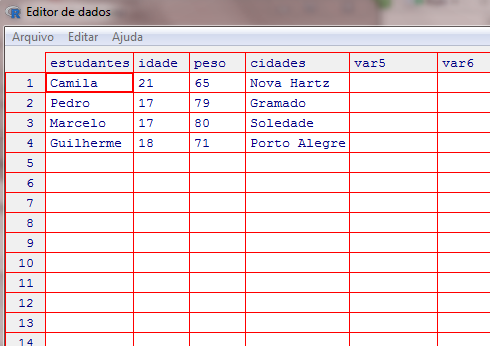
\includegraphics[width=\textwidth]{95} 

}

\caption{Editor de dados}\label{fig:95}
\end{figure}

Basta clicar no retângulo correspondente a variável que deseja ser
modificada, excluir ou adicionar novas colunas.

\begin{figure}

{\centering 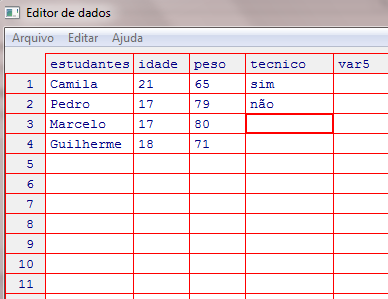
\includegraphics[width=\textwidth]{10} 

}

\caption{Acréscimo de uma nova coluna através do editor de dados}\label{fig:10}
\end{figure}

Logo, chamando o novo banco de dados, teremos:

\begin{Shaded}
\begin{Highlighting}[]
\NormalTok{informacoes}\FloatTok{.2} 
\end{Highlighting}
\end{Shaded}

\begin{verbatim}
  estudantes idade peso      cidades
1     Camila    21   65   Nova Hartz
2      Pedro    17   79      Gramado
3    Marcelo    17   80     Soledade
4  Guilherme    18  100 Porto Alegre
\end{verbatim}

\hypertarget{funcoes}{%
\section{Funções}\label{funcoes}}

As funções a seguir são aplicáveis a vetores, data.frames e listas, e em
muitos casos trazem praticidade a uma análise estatística. Foram criados
objetos com informações do nome dos estudantes e altura. Segue o
processo de criação do \emph{data frame} com estas informações,
lembrando que esta forma de ``união'' das informações pressupõe que a
ordem dos dados esteja correta:

\begin{Shaded}
\begin{Highlighting}[]
\CommentTok{# União de um banco de dados (existencia de uma váriavel em comum)}

\NormalTok{estudantes=}\KeywordTok{c}\NormalTok{(}\StringTok{"Guilherme"}\NormalTok{, }\StringTok{"Marcelo"}\NormalTok{, }\StringTok{"Pedro"}\NormalTok{, }\StringTok{"Camila"}\NormalTok{)}
\NormalTok{altura=}\StringTok{ }\KeywordTok{c}\NormalTok{(}\FloatTok{1.50}\NormalTok{, }\FloatTok{1.9}\NormalTok{, }\FloatTok{1.74}\NormalTok{, }\FloatTok{1.80}\NormalTok{)}
\NormalTok{informacoes}\FloatTok{.3}\NormalTok{=}\KeywordTok{data.frame}\NormalTok{(estudantes, altura)}
\end{Highlighting}
\end{Shaded}

Já o comando \texttt{merge()} serve para juntar dois \emph{data frames}
que possuam uma coluna em comum. Neste caso, unimos o objeto
\texttt{informações.2} com o objeto \texttt{informações.3} utilizando o
nome dos estudantes (informação em comum):

\begin{Shaded}
\begin{Highlighting}[]
\NormalTok{informacoes=}\KeywordTok{merge}\NormalTok{(informacoes}\FloatTok{.2}\NormalTok{,informacoes}\FloatTok{.3}\NormalTok{, }\DataTypeTok{by=}\StringTok{"estudantes"}\NormalTok{)}
\end{Highlighting}
\end{Shaded}

Adicionar um cálculo entre as colunas é muito simples com o RStudio,
neste caso com os dados do peso e altura, pode-se calcular o IMC (Índice
de Massa Corporal) em uma nova coluna:

\begin{Shaded}
\begin{Highlighting}[]
\NormalTok{informacoes}\OperatorTok{$}\NormalTok{Imc=}\KeywordTok{c}\NormalTok{(peso}\OperatorTok{/}\NormalTok{(altura}\OperatorTok{^}\DecValTok{2}\NormalTok{))}
\NormalTok{informacoes}
\end{Highlighting}
\end{Shaded}

\begin{verbatim}
  estudantes idade peso      cidades altura   Imc
1     Camila    21   65   Nova Hartz   1.80 28.89
2  Guilherme    18  100 Porto Alegre   1.50 21.88
3    Marcelo    17   80     Soledade   1.90 26.42
4      Pedro    17   79      Gramado   1.74 30.86
\end{verbatim}

Ainda, se houver linhas que tenham pelo menos uma informação faltante
(NA), estas podem ser excluídas com o comando \texttt{na.omit()}, ou
mesmo os NAs serem substituídos por outro caractere (neste caso foi
substituído por zero) com o comando \texttt{is.na}:

\begin{Shaded}
\begin{Highlighting}[]
\CommentTok{# Retirar as linhas que tenham pelo menos um NA:}

\NormalTok{informacoes<-}\StringTok{ }\KeywordTok{na.omit}\NormalTok{(informacoes)}
\NormalTok{informacoes}
\end{Highlighting}
\end{Shaded}

\begin{verbatim}
  estudantes idade peso      cidades altura   Imc
1     Camila    21   65   Nova Hartz   1.80 28.89
2  Guilherme    18  100 Porto Alegre   1.50 21.88
3    Marcelo    17   80     Soledade   1.90 26.42
4      Pedro    17   79      Gramado   1.74 30.86
\end{verbatim}

\begin{Shaded}
\begin{Highlighting}[]
\CommentTok{# Substituir NA's por zero no data.frame}

\NormalTok{informacoes[}\KeywordTok{is.na}\NormalTok{(informacoes)] =}\StringTok{ }\DecValTok{0}
\NormalTok{informacoes}
\end{Highlighting}
\end{Shaded}

\begin{verbatim}
  estudantes idade peso      cidades altura   Imc
1     Camila    21   65   Nova Hartz   1.80 28.89
2  Guilherme    18  100 Porto Alegre   1.50 21.88
3    Marcelo    17   80     Soledade   1.90 26.42
4      Pedro    17   79      Gramado   1.74 30.86
\end{verbatim}

Outro recurso interessante é a substituição de dados em uma columa, que
pode ser feito de forma automática para uma condição padrão escolhida.
No exemplo abaixo, substituimos aquelas informações de idade igual a 17
pelo número 19:

\begin{Shaded}
\begin{Highlighting}[]
\CommentTok{# Substituir números na coluna}
\NormalTok{informacoes}\OperatorTok{$}\NormalTok{idade[informacoes}\OperatorTok{$}\NormalTok{idade }\OperatorTok{==}\StringTok{ }\DecValTok{17}\NormalTok{] <-}\StringTok{ }\DecValTok{19}
\NormalTok{informacoes}
\end{Highlighting}
\end{Shaded}

\begin{verbatim}
  estudantes idade peso      cidades altura   Imc
1     Camila    21   65   Nova Hartz   1.80 28.89
2  Guilherme    18  100 Porto Alegre   1.50 21.88
3    Marcelo    19   80     Soledade   1.90 26.42
4      Pedro    19   79      Gramado   1.74 30.86
\end{verbatim}

A classificação qualitativa das informações, com base em condições
definidas pelo usuário podem ser facilmente efetuadas pelo comando
\texttt{ifelse}. Para quem não tem intimidade com atributos de
programação, este comando seleciona ``se'' (\emph{if}) uma informação
desejada é atendida, e cria uma rotina (\emph{else}) que será aplicada
``então''.

No nosso exemplo, cria-se um objeto ``classificacao'' e se a coluna IMC
conter dados acima de 25, será marcado como ``peso normal'', sendo que
do contrário, constará como ``excesso de peso''. Após utilizamos o
comando \texttt{cbind()} para unir os dois objetos pelas colunas. caso
não queira utilizar o comando \texttt{cbind()}, poderia ser criado uma
nova coluna com o nome do obetjo sendo ``informacoes\$classificacao''.

\begin{Shaded}
\begin{Highlighting}[]
\CommentTok{# Classificar qualitativamente informações em um determinado intervalo }
\NormalTok{classificacao=}\KeywordTok{ifelse}\NormalTok{(informacoes}\OperatorTok{$}\NormalTok{Imc}\OperatorTok{<}\DecValTok{25}\NormalTok{, }\StringTok{"peso normal"}\NormalTok{, }
                     \StringTok{"excesso de peso"}\NormalTok{)}
\NormalTok{informacoes=}\KeywordTok{cbind}\NormalTok{(informacoes, classificacao)}
\NormalTok{informacoes}
\end{Highlighting}
\end{Shaded}

\begin{verbatim}
  estudantes idade peso      cidades altura   Imc   classificacao
1     Camila    21   65   Nova Hartz   1.80 28.89 excesso de peso
2  Guilherme    18  100 Porto Alegre   1.50 21.88     peso normal
3    Marcelo    19   80     Soledade   1.90 26.42 excesso de peso
4      Pedro    19   79      Gramado   1.74 30.86 excesso de peso
\end{verbatim}

\begin{table}

\caption{\label{tab:imct}Valores padrão para o IMC}
\centering
\begin{tabular}[t]{l|l}
\hline
Resultado & Significado\\
\hline
Abaixo de 17 & Muito abaixo do peso\\
\hline
Entre 17 e 18,49 & Abaixo do peso\\
\hline
Entre 18,5 e 24,99 & Peso normal\\
\hline
Entre 25 e 29,99 & Acima do peso\\
\hline
Entre 30 e 34,99 & Obesidade I\\
\hline
Entre 35 e 39,99 & Obesidade II (severa)\\
\hline
Acima de 40 & Obesidade III (mórbida)\\
\hline
\end{tabular}
\end{table}

No entanto, o IMC possui várias classificações de acordo com o seu
resultado (Tabela \ref{tab:imct}), sendo que, por exemplo, resultados
abaixo de 17 informam que o indivíduo se encontra como Muito abaixo do
peso, e acima de 40, se encontra em Obesidade III. Para efetuar a
classificação desta maneira utilizando o comando \texttt{ifelse}, ou
seja, com mais de uma condição, pode ser efetuada a estruturação com a
aglutinação do comando:

\begin{Shaded}
\begin{Highlighting}[]
\NormalTok{informacoes}\OperatorTok{$}\NormalTok{tipoimc=}\KeywordTok{ifelse}\NormalTok{(informacoes}\OperatorTok{$}\NormalTok{Imc}\OperatorTok{<}\DecValTok{17}\NormalTok{, }\StringTok{"Muito abaixo do peso"}\NormalTok{,}
\KeywordTok{ifelse}\NormalTok{(informacoes}\OperatorTok{$}\NormalTok{Imc}\OperatorTok{>=}\DecValTok{17}\OperatorTok{&}\NormalTok{informacoes}\OperatorTok{$}\NormalTok{Imc}\OperatorTok{<=}\FloatTok{18.49}\NormalTok{,}\StringTok{"Abaixo do peso"}\NormalTok{,}
\KeywordTok{ifelse}\NormalTok{(informacoes}\OperatorTok{$}\NormalTok{Imc}\OperatorTok{>=}\FloatTok{18.5}\OperatorTok{&}\NormalTok{informacoes}\OperatorTok{$}\NormalTok{Imc}\OperatorTok{<=}\FloatTok{24.99}\NormalTok{,}\StringTok{"Peso Normal"}\NormalTok{,}
\KeywordTok{ifelse}\NormalTok{(informacoes}\OperatorTok{$}\NormalTok{Imc}\OperatorTok{>=}\DecValTok{25}\OperatorTok{&}\NormalTok{informacoes}\OperatorTok{$}\NormalTok{Imc}\OperatorTok{<=}\FloatTok{29.99}\NormalTok{,}\StringTok{"Acima do Peso"}\NormalTok{,}
\KeywordTok{ifelse}\NormalTok{(informacoes}\OperatorTok{$}\NormalTok{Imc}\OperatorTok{>=}\DecValTok{30}\OperatorTok{&}\NormalTok{informacoes}\OperatorTok{$}\NormalTok{Imc}\OperatorTok{<=}\FloatTok{34.99}\NormalTok{,}\StringTok{"Obesidade I"}\NormalTok{,}
\KeywordTok{ifelse}\NormalTok{(informacoes}\OperatorTok{$}\NormalTok{Imc}\OperatorTok{>=}\DecValTok{35}\OperatorTok{&}\NormalTok{informacoes}\OperatorTok{$}\NormalTok{Imc}\OperatorTok{<=}\FloatTok{39.99}\NormalTok{,}\StringTok{"Obesidade II"}\NormalTok{,}
       \StringTok{"Obesidade III"}\NormalTok{))))))}
\NormalTok{informacoes}
\end{Highlighting}
\end{Shaded}

\begin{verbatim}
  estudantes idade peso      cidades altura   Imc   classificacao       tipoimc
1     Camila    21   65   Nova Hartz   1.80 28.89 excesso de peso Acima do Peso
2  Guilherme    18  100 Porto Alegre   1.50 21.88     peso normal   Peso Normal
3    Marcelo    19   80     Soledade   1.90 26.42 excesso de peso Acima do Peso
4      Pedro    19   79      Gramado   1.74 30.86 excesso de peso   Obesidade I
\end{verbatim}

A classificação binária dos dados (0,1) também é relevante para o estudo
da manipulação dos dados trabalhados pelo pesquisador. Neste exemplo,
classificou-se aqueles valores da coluna ``classificacao'' com o ``peso
normal'' iguais a 1, do contrário classificou-se 0 (zero).

\begin{Shaded}
\begin{Highlighting}[]
\CommentTok{# Classificar informações usando o código binário}
\NormalTok{informacoes}\OperatorTok{$}\NormalTok{binario=}\StringTok{ }\KeywordTok{ifelse}\NormalTok{(informacoes}\OperatorTok{$}\NormalTok{classificacao }
                            \OperatorTok{==}\StringTok{ 'peso normal'}\NormalTok{, }\DecValTok{1}\NormalTok{, }\DecValTok{0}\NormalTok{) }
\NormalTok{informacoes}
\end{Highlighting}
\end{Shaded}

\begin{verbatim}
  estudantes idade peso      cidades altura   Imc   classificacao       tipoimc
1     Camila    21   65   Nova Hartz   1.80 28.89 excesso de peso Acima do Peso
2  Guilherme    18  100 Porto Alegre   1.50 21.88     peso normal   Peso Normal
3    Marcelo    19   80     Soledade   1.90 26.42 excesso de peso Acima do Peso
4      Pedro    19   79      Gramado   1.74 30.86 excesso de peso   Obesidade I
  binario
1       0
2       1
3       0
4       0
\end{verbatim}

O comando \texttt{rbind()} é utilizado para incluir linhas novas abaixo
de um objeto já criado pelo pesquisador, sendo que é importante o
cuidado de que estas novas informações tenham os mesmos campos
(colunas). A exemplo, pede-se para incluir uma nova pessoa no \emph{data
frame} informacoes: Francisco, 30 anos de idade, peso 59, natural de
Ijuí, IMC 21.3387, classificado como peso normal. Lembrando de incluir
os campos ``tipoimc'' e ``binario''.

\begin{Shaded}
\begin{Highlighting}[]
\NormalTok{novo1=}\KeywordTok{data.frame}\NormalTok{(}\DataTypeTok{estudantes=}\StringTok{"Francisco"}\NormalTok{, }\DataTypeTok{idade=}\DecValTok{30}\NormalTok{, }\DataTypeTok{peso=}\DecValTok{59}\NormalTok{, }
                 \DataTypeTok{cidades=}\StringTok{"Ijuí"}\NormalTok{, }
                 \DataTypeTok{altura=}\StringTok{"1,59"}\NormalTok{, }
                 \DataTypeTok{Imc=} \FloatTok{23.30}\NormalTok{, }
                 \DataTypeTok{classificacao=} \StringTok{"peso normal"}\NormalTok{,}
                 \DataTypeTok{tipoimc=}\StringTok{"Peso Normal"}\NormalTok{, }
                 \DataTypeTok{binario=}\DecValTok{1}\NormalTok{)}
\NormalTok{informacoes=}\KeywordTok{rbind}\NormalTok{(informacoes, novo1)}
\NormalTok{informacoes}
\end{Highlighting}
\end{Shaded}

\begin{verbatim}
  estudantes idade peso      cidades altura   Imc   classificacao       tipoimc
1     Camila    21   65   Nova Hartz    1.8 28.89 excesso de peso Acima do Peso
2  Guilherme    18  100 Porto Alegre    1.5 21.88     peso normal   Peso Normal
3    Marcelo    19   80     Soledade    1.9 26.42 excesso de peso Acima do Peso
4      Pedro    19   79      Gramado   1.74 30.86 excesso de peso   Obesidade I
5  Francisco    30   59         Ijuí   1,59 23.30     peso normal   Peso Normal
  binario
1       0
2       1
3       0
4       0
5       1
\end{verbatim}

Outra forma de incluir informações adicionais nos \emph{data frames}
através de atributos é utilizando o pacote \texttt{dplyr}. Decide-se
criar um campo ``faixa etária'', sendo que aqueles indivíduos com idade
acima de 21 chamaremos de ``adulto'' e do contrário ``não adulto''.

\begin{Shaded}
\begin{Highlighting}[]
\KeywordTok{require}\NormalTok{(dplyr)}
\end{Highlighting}
\end{Shaded}

\begin{verbatim}
Carregando pacotes exigidos: dplyr
\end{verbatim}

\begin{verbatim}

Attaching package: 'dplyr'
\end{verbatim}

\begin{verbatim}
The following objects are masked from 'package:stats':

    filter, lag
\end{verbatim}

\begin{verbatim}
The following objects are masked from 'package:base':

    intersect, setdiff, setequal, union
\end{verbatim}

\begin{Shaded}
\begin{Highlighting}[]
\NormalTok{informacoes=}\StringTok{ }\KeywordTok{mutate}\NormalTok{(informacoes, }
                    \StringTok{"faixa etaria"}\NormalTok{=}\StringTok{ }\KeywordTok{ifelse}\NormalTok{(informacoes}\OperatorTok{$}\NormalTok{idade}\OperatorTok{<}\DecValTok{21}\NormalTok{,}
                                           \StringTok{"não adulto"}\NormalTok{, }\StringTok{"adulto"}\NormalTok{))}
\NormalTok{informacoes}
\end{Highlighting}
\end{Shaded}

\begin{verbatim}
  estudantes idade peso      cidades altura   Imc   classificacao       tipoimc
1     Camila    21   65   Nova Hartz    1.8 28.89 excesso de peso Acima do Peso
2  Guilherme    18  100 Porto Alegre    1.5 21.88     peso normal   Peso Normal
3    Marcelo    19   80     Soledade    1.9 26.42 excesso de peso Acima do Peso
4      Pedro    19   79      Gramado   1.74 30.86 excesso de peso   Obesidade I
5  Francisco    30   59         Ijuí   1,59 23.30     peso normal   Peso Normal
  binario faixa etaria
1       0       adulto
2       1   não adulto
3       0   não adulto
4       0   não adulto
5       1       adulto
\end{verbatim}

A (re)ordenação das colunas de um \emph{data frame} pode ser muito útil
em alguns casos, sendo extremamente fácil efetuá-la, cada número
representa o número da respectiva coluna:

\begin{Shaded}
\begin{Highlighting}[]
\CommentTok{# Reordenar colunas}
\NormalTok{informacoes=informacoes[}\KeywordTok{c}\NormalTok{(}\DecValTok{8}\NormalTok{,}\DecValTok{2}\NormalTok{,}\DecValTok{3}\NormalTok{,}\DecValTok{4}\NormalTok{,}\DecValTok{1}\NormalTok{,}\DecValTok{6}\NormalTok{,}\DecValTok{5}\NormalTok{,}\DecValTok{7}\NormalTok{,}\DecValTok{9}\NormalTok{)]}
\end{Highlighting}
\end{Shaded}

Caso se queira a inversão total da ordem das colunas do objeto estudado,
o comando \texttt{rev()} pode ser útil:

\begin{Shaded}
\begin{Highlighting}[]
\CommentTok{# Inversão do posicionamento dos elementos}
\KeywordTok{rev}\NormalTok{(informacoes)}
\end{Highlighting}
\end{Shaded}

\begin{verbatim}
  binario   classificacao altura   Imc estudantes      cidades peso idade
1       0 excesso de peso    1.8 28.89     Camila   Nova Hartz   65    21
2       1     peso normal    1.5 21.88  Guilherme Porto Alegre  100    18
3       0 excesso de peso    1.9 26.42    Marcelo     Soledade   80    19
4       0 excesso de peso   1.74 30.86      Pedro      Gramado   79    19
5       1     peso normal   1,59 23.30  Francisco         Ijuí   59    30
        tipoimc
1 Acima do Peso
2   Peso Normal
3 Acima do Peso
4   Obesidade I
5   Peso Normal
\end{verbatim}

A função \texttt{table()} faz a contagem os dados; já o comando
\texttt{sort()} ordena os objetos em ordem crescente (caso queira no
formato decrescente, informar \texttt{decreasing=TRUE}).

\begin{Shaded}
\begin{Highlighting}[]
\CommentTok{# contagem de objetos}
\KeywordTok{table}\NormalTok{(informacoes}\OperatorTok{$}\NormalTok{classificacao)}
\end{Highlighting}
\end{Shaded}

\begin{verbatim}

excesso de peso     peso normal 
              3               2 
\end{verbatim}

\begin{Shaded}
\begin{Highlighting}[]
\CommentTok{# Ordenar os objetos em ordem crescente}
\KeywordTok{sort}\NormalTok{(informacoes}\OperatorTok{$}\NormalTok{idade)}
\end{Highlighting}
\end{Shaded}

\begin{verbatim}
[1] 18 19 19 21 30
\end{verbatim}

A ordenação de todo o \emph{data frame} a partir de uma variável, pode
ser realizada utilizando o comando \texttt{order}, sendo que pode ser
realizada inclusive com variáveis categóricas (no exemplo abaixo o nome
das cidades).

\begin{Shaded}
\begin{Highlighting}[]
\CommentTok{# Ordem decrescente }
\NormalTok{informacoes[}\KeywordTok{order}\NormalTok{(informacoes}\OperatorTok{$}\NormalTok{idade, }\DataTypeTok{decreasing =} \OtherTok{TRUE}\NormalTok{),]}
\end{Highlighting}
\end{Shaded}

\begin{verbatim}
        tipoimc idade peso      cidades estudantes   Imc altura   classificacao
5   Peso Normal    30   59         Ijuí  Francisco 23.30   1,59     peso normal
1 Acima do Peso    21   65   Nova Hartz     Camila 28.89    1.8 excesso de peso
3 Acima do Peso    19   80     Soledade    Marcelo 26.42    1.9 excesso de peso
4   Obesidade I    19   79      Gramado      Pedro 30.86   1.74 excesso de peso
2   Peso Normal    18  100 Porto Alegre  Guilherme 21.88    1.5     peso normal
  binario
5       1
1       0
3       0
4       0
2       1
\end{verbatim}

\begin{Shaded}
\begin{Highlighting}[]
\CommentTok{#ordem crescente}
\NormalTok{informacoes[}\KeywordTok{order}\NormalTok{(informacoes}\OperatorTok{$}\NormalTok{idade, }\DataTypeTok{decreasing =} \OtherTok{FALSE}\NormalTok{),]}
\end{Highlighting}
\end{Shaded}

\begin{verbatim}
        tipoimc idade peso      cidades estudantes   Imc altura   classificacao
2   Peso Normal    18  100 Porto Alegre  Guilherme 21.88    1.5     peso normal
3 Acima do Peso    19   80     Soledade    Marcelo 26.42    1.9 excesso de peso
4   Obesidade I    19   79      Gramado      Pedro 30.86   1.74 excesso de peso
1 Acima do Peso    21   65   Nova Hartz     Camila 28.89    1.8 excesso de peso
5   Peso Normal    30   59         Ijuí  Francisco 23.30   1,59     peso normal
  binario
2       1
3       0
4       0
1       0
5       1
\end{verbatim}

\begin{Shaded}
\begin{Highlighting}[]
\CommentTok{#ordem crescente}
\NormalTok{informacoes[}\KeywordTok{order}\NormalTok{(informacoes}\OperatorTok{$}\NormalTok{cidades, }\DataTypeTok{decreasing =} \OtherTok{FALSE}\NormalTok{),]}
\end{Highlighting}
\end{Shaded}

\begin{verbatim}
        tipoimc idade peso      cidades estudantes   Imc altura   classificacao
4   Obesidade I    19   79      Gramado      Pedro 30.86   1.74 excesso de peso
5   Peso Normal    30   59         Ijuí  Francisco 23.30   1,59     peso normal
1 Acima do Peso    21   65   Nova Hartz     Camila 28.89    1.8 excesso de peso
2   Peso Normal    18  100 Porto Alegre  Guilherme 21.88    1.5     peso normal
3 Acima do Peso    19   80     Soledade    Marcelo 26.42    1.9 excesso de peso
  binario
4       0
5       1
1       0
2       1
3       0
\end{verbatim}

O comando \texttt{rank()} cria uma ranqueamento crescente das
informações. Se pretende-se, por exemplo, criar uma coluna com o ranking
dos valores do IMC, pode ser utilizado:

\begin{Shaded}
\begin{Highlighting}[]
\NormalTok{informacoes}\OperatorTok{$}\NormalTok{rankingImc=}\KeywordTok{rank}\NormalTok{(informacoes}\OperatorTok{$}\NormalTok{Imc)}
\NormalTok{informacoes}
\end{Highlighting}
\end{Shaded}

\begin{verbatim}
        tipoimc idade peso      cidades estudantes   Imc altura   classificacao
1 Acima do Peso    21   65   Nova Hartz     Camila 28.89    1.8 excesso de peso
2   Peso Normal    18  100 Porto Alegre  Guilherme 21.88    1.5     peso normal
3 Acima do Peso    19   80     Soledade    Marcelo 26.42    1.9 excesso de peso
4   Obesidade I    19   79      Gramado      Pedro 30.86   1.74 excesso de peso
5   Peso Normal    30   59         Ijuí  Francisco 23.30   1,59     peso normal
  binario rankingImc
1       0          4
2       1          1
3       0          3
4       0          5
5       1          2
\end{verbatim}

\hypertarget{funcoes-matematicas}{%
\section{Funções Matemáticas}\label{funcoes-matematicas}}

A utilização de funções matemáticasno RStudio contribui para que o
pesquisador possa realizar vários experimentos com seus dados. Os
cálculos podem ser efetuados diretamente no console do programa ou
aplicados aos objetos criados:

\begin{Shaded}
\begin{Highlighting}[]
\KeywordTok{log}\NormalTok{(}\FloatTok{1.5}\NormalTok{)}
\end{Highlighting}
\end{Shaded}

\begin{verbatim}
[1] 0.4055
\end{verbatim}

\begin{Shaded}
\begin{Highlighting}[]
\KeywordTok{exp}\NormalTok{(}\DecValTok{1}\NormalTok{)}
\end{Highlighting}
\end{Shaded}

\begin{verbatim}
[1] 2.718
\end{verbatim}

No caso do \emph{data frame} o qual foi criado acima (``informacoes''),
pode-se buscar as informações dos valores mínimos (função
\texttt{min()}), máximos (\texttt{max()}) da base:

\begin{Shaded}
\begin{Highlighting}[]
\KeywordTok{max}\NormalTok{(informacoes}\OperatorTok{$}\NormalTok{idade)}
\end{Highlighting}
\end{Shaded}

\begin{verbatim}
[1] 30
\end{verbatim}

\begin{Shaded}
\begin{Highlighting}[]
\KeywordTok{min}\NormalTok{(informacoes}\OperatorTok{$}\NormalTok{idade)}
\end{Highlighting}
\end{Shaded}

\begin{verbatim}
[1] 18
\end{verbatim}

Ainda, se o interesse está em descobrir a posição, no *data frame\}, do
peso mínimo e máximo da amostra utiliza-se o comando \texttt{which.min}
e \texttt{which.max}.

\begin{Shaded}
\begin{Highlighting}[]
\CommentTok{# Para descobrir em qual posição se encontra o peso mínimo:}
\KeywordTok{which.min}\NormalTok{(informacoes}\OperatorTok{$}\NormalTok{peso)}
\end{Highlighting}
\end{Shaded}

\begin{verbatim}
[1] 5
\end{verbatim}

\begin{Shaded}
\begin{Highlighting}[]
\KeywordTok{which.max}\NormalTok{(informacoes}\OperatorTok{$}\NormalTok{peso)}
\end{Highlighting}
\end{Shaded}

\begin{verbatim}
[1] 2
\end{verbatim}

Para descobrir qual é o estutande que possui o peso mínimo, por exemplo,
ou o Imc máximo, utiliza-se o seguinte comando (notem que os resultados
trazem a lista de todos os estudantes comparados):

\begin{Shaded}
\begin{Highlighting}[]
\NormalTok{informacoes}\OperatorTok{$}\NormalTok{estudantes[}\KeywordTok{which.min}\NormalTok{(informacoes}\OperatorTok{$}\NormalTok{peso)]}
\end{Highlighting}
\end{Shaded}

\begin{verbatim}
[1] Francisco
Levels: Camila Guilherme Marcelo Pedro Francisco
\end{verbatim}

\begin{Shaded}
\begin{Highlighting}[]
\NormalTok{informacoes}\OperatorTok{$}\NormalTok{estudantes[}\KeywordTok{which.max}\NormalTok{(informacoes}\OperatorTok{$}\NormalTok{Imc)]}
\end{Highlighting}
\end{Shaded}

\begin{verbatim}
[1] Pedro
Levels: Camila Guilherme Marcelo Pedro Francisco
\end{verbatim}

O arredondamento de valores numéricos pode ser feito utilizando o
comando \texttt{round()}, o qual o pesquisador informa o número de casas
decimais:

\begin{Shaded}
\begin{Highlighting}[]
\CommentTok{# Arredondar para n casas decimais}
\KeywordTok{round}\NormalTok{(informacoes}\OperatorTok{$}\NormalTok{Imc, }\DecValTok{2}\NormalTok{)}
\end{Highlighting}
\end{Shaded}

\begin{verbatim}
[1] 28.89 21.88 26.42 30.86 23.30
\end{verbatim}

Já o comando \texttt{signif()} determina onúmero de algarismos
significativos da série escolhida, ou seja, ele arredonda para os
valores em seu primeiro argumento com os número de dígitos detemrinados:

\begin{Shaded}
\begin{Highlighting}[]
\NormalTok{x2 <-}\StringTok{ }\NormalTok{pi }\OperatorTok{*}\StringTok{ }\DecValTok{100}\OperatorTok{^}\NormalTok{(}\OperatorTok{-}\DecValTok{1}\OperatorTok{:}\DecValTok{3}\NormalTok{)}
\KeywordTok{round}\NormalTok{(x2, }\DecValTok{3}\NormalTok{)}
\end{Highlighting}
\end{Shaded}

\begin{verbatim}
[1] 3.100e-02 3.142e+00 3.142e+02 3.142e+04 3.142e+06
\end{verbatim}

\begin{Shaded}
\begin{Highlighting}[]
\KeywordTok{signif}\NormalTok{(x2, }\DecValTok{3}\NormalTok{) }
\end{Highlighting}
\end{Shaded}

\begin{verbatim}
[1] 3.14e-02 3.14e+00 3.14e+02 3.14e+04 3.14e+06
\end{verbatim}

A soma do total da coluna idade, o desvio padrão, a variância, a média
aritmética e mediana podem ser encontrados, respectivamente, pelos
comandos \texttt{sum()}, \texttt{sd()}, \texttt{var()}, \texttt{mean()},
\texttt{median()}:

\begin{Shaded}
\begin{Highlighting}[]
\CommentTok{# Realiza a somatória dos valores}
\KeywordTok{sum}\NormalTok{(informacoes}\OperatorTok{$}\NormalTok{idade)}
\end{Highlighting}
\end{Shaded}

\begin{verbatim}
[1] 107
\end{verbatim}

\begin{Shaded}
\begin{Highlighting}[]
\CommentTok{# Desvio padrão}
\KeywordTok{sd}\NormalTok{(informacoes}\OperatorTok{$}\NormalTok{idade)}
\end{Highlighting}
\end{Shaded}

\begin{verbatim}
[1] 4.93
\end{verbatim}

\begin{Shaded}
\begin{Highlighting}[]
\CommentTok{# Variancia}
\KeywordTok{var}\NormalTok{(informacoes}\OperatorTok{$}\NormalTok{idade)}
\end{Highlighting}
\end{Shaded}

\begin{verbatim}
[1] 24.3
\end{verbatim}

\begin{Shaded}
\begin{Highlighting}[]
\CommentTok{# Calcula a média aritmética dos valores}
\KeywordTok{mean}\NormalTok{(informacoes}\OperatorTok{$}\NormalTok{idade)}
\end{Highlighting}
\end{Shaded}

\begin{verbatim}
[1] 21.4
\end{verbatim}

\begin{Shaded}
\begin{Highlighting}[]
\CommentTok{# Informa o valor mediano do conjunto}
\KeywordTok{median}\NormalTok{(informacoes}\OperatorTok{$}\NormalTok{idade)}
\end{Highlighting}
\end{Shaded}

\begin{verbatim}
[1] 19
\end{verbatim}

O comando \texttt{quantile()} oferece a possibilidade de obter os
quartis dos dados de acordo com as probabilidades estabelecidas pelo
pesquisador. No exemplo, explora-se a variável idade:

\begin{Shaded}
\begin{Highlighting}[]
\KeywordTok{quantile}\NormalTok{(informacoes}\OperatorTok{$}\NormalTok{idade,  }\DataTypeTok{probs =} \KeywordTok{c}\NormalTok{(}\FloatTok{0.5}\NormalTok{, }\DecValTok{1}\NormalTok{, }\DecValTok{2}\NormalTok{, }\DecValTok{5}\NormalTok{, }\DecValTok{10}\NormalTok{, }\DecValTok{50}\NormalTok{)}\OperatorTok{/}\DecValTok{100}\NormalTok{)}
\end{Highlighting}
\end{Shaded}

\begin{verbatim}
 0.5%    1%    2%    5%   10%   50% 
18.02 18.04 18.08 18.20 18.40 19.00 
\end{verbatim}

\hypertarget{conversao-de-datas}{%
\section{Conversão de datas}\label{conversao-de-datas}}

A configuração e padronização dos formato de datas no RStudio podem ser
efetuadas pelo pesquisador, primeiramente ao carregar a base de dados no
programa e em um segundo momento durante a manipulação das informações.
Assim, seguem alguns dos procedimentos para a correta alteração dos
padrões de datas:

\begin{Shaded}
\begin{Highlighting}[]
\NormalTok{abertura <-}\StringTok{ }\KeywordTok{c}\NormalTok{(}\StringTok{"03/02/69"}\NormalTok{, }\StringTok{"17/08/67"}\NormalTok{)}
\NormalTok{fechamento <-}\StringTok{ }\KeywordTok{c}\NormalTok{(}\StringTok{"2000-20-01"}\NormalTok{, }\StringTok{"1999-14-08"}\NormalTok{)}
\NormalTok{abertura <-}\StringTok{ }\KeywordTok{as.Date}\NormalTok{(abertura, }\DataTypeTok{format =} \StringTok{"%d/%m/%y"}\NormalTok{)}
\NormalTok{fechamento <-}\StringTok{ }\KeywordTok{as.Date}\NormalTok{(fechamento, }\DataTypeTok{format =} \StringTok{"%Y-%d-%m"}\NormalTok{)}

\CommentTok{# Diferença de dias dos intervalos informados}
\NormalTok{abertura}\OperatorTok{-}\NormalTok{fechamento}
\end{Highlighting}
\end{Shaded}

\begin{verbatim}
Time differences in days
[1] -11308  24840
\end{verbatim}

\hypertarget{desc}{%
\chapter{Estatística Descritiva}\label{desc}}

A Estatística é uma ciência cujo campo de aplicação estende-se a
diferentes áreas do conhecimento humano. Tem por objetivo fornecer
métodos e técnicas que permitem lidar, racionalmente, com situações
sujeitas a incertezas. Apresenta um conjunto de técnicas e métodos de
pesquisa que envolvem o planejamento de estudos (experimentais e
observacionais), a coleta e organização de dados, a inferência, a
análise e a disseminação de informação.

Alguns termos extensamente utilizados em estatística, são definidos a
seguir \autocite{triola1999}:

\textbf{População}: é uma coleção completa de todos os elementos
(valores, pessoas, medidas etc.) a serem estudados.

\textbf{Censo}: é uma coleção de dados relativos a todos os elementos de
uma população.

\textbf{Amostra}: é uma sub-coleção de elementos extraídos de uma
população. Parâmetro é a medida numérica que descreve uma característica
de uma população.

\textbf{Estatística}: é uma medida numérica que descreve uma
característica de uma amostra.

\hypertarget{natureza-da-medida-das-variaveis}{%
\section{Natureza da medida das
variáveis}\label{natureza-da-medida-das-variaveis}}

Variáveis reporta-se a características ou atributos que podem tomar
diferentes valores ou categorias, o que se opõe ao conceito de constante
\autocite{almeida2000}. Assim, variável pode ser definida como sendo a
característica dos elementos da amostra ou da população que nos
interessa estudar estatisticamente.

Variáveis podem ser classificadas da seguinte forma:

\textbf{Variáveis quantitativas}: consistem em números que representam
contagens ou medidas. Dividem-se em:

\begin{enumerate}
\def\labelenumi{\alph{enumi})}
\item
  Variáveis discretas: resultam em um conjunto finito de valores
  possíveis, ou de um conjunto enumerável desses valores. Ex. número de
  unidades produzidas.
\item
  Variáveis contínuas: resultam de um número infinito de valores
  possíveis que podem ser associados a pontos em uma escala contínua de
  tal maneira que não haja lacunas ou interrupções. Ex. Renda das
  famílias em reais.
\end{enumerate}

\textbf{Variáveis qualitativas}: ou variáveis categóricas, ou atributos
que podem ser separados em diferentes categorias que se distinguem por
alguma característica não-numérica. Divididas em:

\begin{enumerate}
\def\labelenumi{\alph{enumi})}
\item
  Variável nominal: caracterizada por dados que consistem apenas em
  nomes, rótulos ou categorias. Os dados não podem ser dispostos segundo
  um esquema ordenado (como de baixo para cima). Ex. nacionalidade
\item
  Variável ordinal: envolve variáveis representadas por nomes que podem
  ser dispostos em alguma ordem, mas as diferenças entre os valores dos
  dados não podem ser determinadas, ou não tem sentido. Esse nível dá
  informações sobre comparações relativas, mas os graus de diferença não
  servem para cálculos \autocite{triola1999}. Ex. Grau de escolaridade.
\end{enumerate}

\textbf{Dado}: é o valor assumido por uma variável aleatória em um
experimento.

A Estatística subdivide-se em descritiva e inferencial. A estatística
descritiva se preocupa em descrever os dados. A estatística inferencial,
fundamentada na teoria das probabilidades, se preocupa com a análise
destes dados e sua interpretação.

Informações estatísticas em jornais, relatórios e outras publicações que
consistem de dados reunidos e apresentados de forma clara e resumida, na
forma de tabelas, gráficos ou numéricos, são conhecidos como
estatísticas descritivas (ANDERSON, 2002).

\textbf{Exemplo 1}

Estaremos utilizando como exemplo os dados de uma pesquisa (dados
simulados), cujo banco de dados está intitulado ``Dados\_pesquisa.ods''.
Os dados são referentes aos resultados obtidos por ocasião de uma
pesquisa realizada entre os consumidores a fim de analisar
características associadas ao mercado consumidor de sucos, sendo que a
amostra é composta de 348 entrevistados aleatoriamente selecionados.

\begin{itemize}
\item
  O objetivo primário do estudo foi determinar variáveis que seriam
  úteis para caracterizar os consumidores que já conhecem o suco e a
  possibilidade potencial de futuros consumidores. Há também interesse
  nas relações entre variáveis das características pessoais desses
  consumidores ou futuros consumidores.
\item
  A pesquisa foi realizada, depois que os participantes realizaram uma
  visita técnica às instalações da empresa e puderam conhecer seus
  produtos e processos.
\end{itemize}

Para cada entrevistado foram registrados dados para as seguintes
variáveis:

\textbf{Sexo} -- Gênero sexual;

\textbf{Divulgacao} -- Forma de acesso ao suco ou publicidade do mesmo;

\textbf{Renda\_h} -- Renda por hora do entrevistado;

\textbf{Praticidade} -- Aspectos quanto a oferta do suco, como por ex.
embalagem;

\textbf{Sabor} -- Aspectos relacionados ao sabor;

\textbf{Pessoas\_familia} -- Número de pessoas que compõe o grupo
familiar;

\textbf{Preço} -- como cada entrevistado classificava o preço do
produto;

\textbf{consumo\_anterior} -- Se já consumia o suco antes da visita
técnica;

\textbf{consumo\_pos} -- Se consumia o suco após a visita técnica;

\textbf{Idade} -- Idade dos consumidores;

\textbf{Altura\_(m)} -- Altura dos consumidores;

\textbf{Peso\_(Kg)} -- Peso dos consumidores.

Pede-se:

\begin{enumerate}
\def\labelenumi{\arabic{enumi}.}
\item
  Salvar inicialmente os dados em formato CSV, xlsx ou outro.
\item
  Ler os dados no ``Environment'' pelo ``Import Dataset\ldots{}From
  CSV'' ou outro. No exemplo abaixo foram importados os dados
  diretamente do arquivo hospedado na internet.
\item
  Carregar o banco de dados, com a finalidade de usar os objetos
  (variáveis) diretamente nas funções a serem utilizadas.
\end{enumerate}

\texttt{attach(nome\_da\_planilha)}

\begin{Shaded}
\begin{Highlighting}[]
\KeywordTok{require}\NormalTok{(readxl)}
\end{Highlighting}
\end{Shaded}

\begin{verbatim}
Carregando pacotes exigidos: readxl
\end{verbatim}

\begin{Shaded}
\begin{Highlighting}[]
\NormalTok{url <-}\StringTok{ "https://goo.gl/37Fdzz"}
\NormalTok{destfile <-}\StringTok{ "pesquisa_dados.xlsx"}
\NormalTok{curl}\OperatorTok{::}\KeywordTok{curl_download}\NormalTok{(url, destfile)}
\NormalTok{pesquisa_dados <-}\StringTok{ }\KeywordTok{read_excel}\NormalTok{(destfile)}
\KeywordTok{attach}\NormalTok{(pesquisa_dados)}
\KeywordTok{ls.str}\NormalTok{(pesquisa_dados)}
\end{Highlighting}
\end{Shaded}

\begin{verbatim}
Altura_(m) :  num [1:348] 1.82 1.9 1.69 1.89 1.9 1.76 1.83 1.81 1.67 1.55 ...
Caso :  num [1:348] 1 2 3 4 5 6 7 8 9 10 ...
consumo_anterior :  chr [1:348] "N" "N" "S" "N" "S" "S" "S" "N" "N" "N" "N" "N" "S" "S" "S" ...
consumo_pos :  chr [1:348] "N" "S" "N" "S" "N" "S" "N" "S" "N" "S" "S" "S" "S" "S" "S" ...
Divulgacao :  chr [1:348] "Degustacao" "Radio" "TV" "TV" "Degustacao" "TV" "TV" "Radio" ...
Idade :  num [1:348] 22 21 20 18 16 28 19 19 22 19 ...
Peso_(Kg) :  num [1:348] 78.5 80 54 78 36 82 75 69 58 49 ...
Pessoas_familia :  num [1:348] 4 3 3 7 4 4 3 4 1 4 ...
Praticidade :  chr [1:348] "Pessima" "Otima" "Boa" "Pessima" "Ruim" "Boa" "Regular" ...
Preço :  chr [1:348] "Acima_concorrencia" "Abaixo_concorrencia" ...
Renda_h :  chr [1:348] "1.41" "17.34" "6.86" "2.65" "2.01" "11.32" "6.86" "3.25" ...
Sabor :  chr [1:348] "Otimo" "Pessimo" "Bom" "Otimo" "Otimo" "Regular" "Ruim" "Bom" ...
Sexo :  chr [1:348] "Feminino" "Feminino" "Feminino" "Feminino" "Masculino" ...
\end{verbatim}

\hypertarget{tabelas-e-graficos}{%
\section{Tabelas e Gráficos}\label{tabelas-e-graficos}}

Segundo \textcite{barbetta1988}, dados representados em tabelas e
gráficos adequados, permitem observar determinados aspectos relevantes,
bem como delinear hipóteses a respeito da estrutura dos dados em estudo,
o que conhecemos como análise exploratória de dados. Isto pode ser feito
inicialmente com a representação em forma de tabelas.

O comando \texttt{table()} é utilizado para elaborarmos tabelas de
frequências absolutas. Dependendo da variável a ser representada,
podemos usar esse comando de diferentes formas:

\hypertarget{tabela-simples-para-apresentacao-das-frequencias-absolutas}{%
\subsection{Tabela simples para apresentação das frequências
absolutas}\label{tabela-simples-para-apresentacao-das-frequencias-absolutas}}

Uma tabela simples considera quantas vezes ocorre cada categoria (ou
nível).

\texttt{table(nome\_variável)}

Ex. Variável \textbf{Praticidade}

\begin{Shaded}
\begin{Highlighting}[]
\KeywordTok{table}\NormalTok{(Praticidade)}
\end{Highlighting}
\end{Shaded}

\begin{verbatim}
Praticidade
    Boa   Otima Pessima Regular    Ruim 
     82      70      21      80      95 
\end{verbatim}

\hypertarget{tabela-cruzada}{%
\subsection{Tabela cruzada}\label{tabela-cruzada}}

A tabela cruzada, também conhecida como tabela de dupla entrada, para
apresentação das frequências absolutas.

\texttt{table(nome\_variável1,nome\_variável2)}

Ex. Construir uma tabela cruzada apresentando as frequências absolutas
das variáveis \textbf{Sexo} e \textbf{Divulgacao}.

\begin{Shaded}
\begin{Highlighting}[]
\KeywordTok{table}\NormalTok{(pesquisa_dados}\OperatorTok{$}\NormalTok{Sexo,pesquisa_dados}\OperatorTok{$}\NormalTok{Divulgacao)}
\end{Highlighting}
\end{Shaded}

\begin{verbatim}
           
            Degustacao Outro Radio  TV
  Feminino          78     6    61 147
  Masculino         19     1    15  21
\end{verbatim}

\hypertarget{tabela-cruzada-para-apresentacao-das-frequencias-relativas}{%
\subsection{Tabela cruzada para apresentação das frequências
relativas}\label{tabela-cruzada-para-apresentacao-das-frequencias-relativas}}

Com a introdução do comando `prop.table\textbar{} é possível gerar,
facilmente, tabelas de frequências relativas para as variáveis de
interesse. As medidas relativas são importantes para comparar
distribuições de frequências \autocite{barbetta1988}.

\texttt{prop.table(table(nome\_variável1,nome\_variável2))}

Ex. Construir uma tabela cruzada apresentando as frequências relativas
das variáveis \textbf{Sexo} e \textbf{Divulgacao}.

\begin{Shaded}
\begin{Highlighting}[]
\KeywordTok{prop.table}\NormalTok{(}\KeywordTok{table}\NormalTok{(Divulgacao,Sexo))}
\end{Highlighting}
\end{Shaded}

\begin{verbatim}
            Sexo
Divulgacao   Feminino Masculino
  Degustacao 0.224138  0.054598
  Outro      0.017241  0.002874
  Radio      0.175287  0.043103
  TV         0.422414  0.060345
\end{verbatim}

A função \texttt{tapply} serve para calcular um valor usando uma
variável categórica como condição, ou seja, aplica uma função qualquer
(como média, por exemplo) a uma variável quantitativa para cada classe
de uma variável categórica. Assim, permite obter em um só comando, a
medida para cada categoria.

\texttt{tapply(var\_quantitativa,var\_categórica,\ função\_desejada)}

\texttt{tapply(variavel\_quantitativa,variavel\_qualitativa,\ mean)}

Se um registro possui \texttt{NA}, isto é, dados perdidos: com o
parâmetro na.rm=T, indicamos para o comando ignorar os NAs nos dados e
calcular a média.

\texttt{tapply(variavel\_quanti,\ variavel\_quali,\ mean,\ na.rm=T)}

\hypertarget{graficos}{%
\section{Gráficos}\label{graficos}}

\hypertarget{grafico-de-colunas}{%
\subsection{Gráfico de colunas}\label{grafico-de-colunas}}

As frequências podem ser visualizadas graficamente, usando gráficos de
barras elementares, que se aplicam à descrição de qualquer variável
qualitativa ou quantitativa discreta, vetor de dados ou tabelas.

No entanto, no caso de dados em banco de dados, quando não utilizamos
outros mecanismos de atribuição, precisamos usar o comando table.

\texttt{barplot(table(nome\_variável))}

Ex. Construir um gráfico de colunas para a variável \textbf{Sexo}.

\begin{Shaded}
\begin{Highlighting}[]
\KeywordTok{barplot}\NormalTok{(}\KeywordTok{table}\NormalTok{(Sexo))}
\end{Highlighting}
\end{Shaded}

\begin{figure}

{\centering 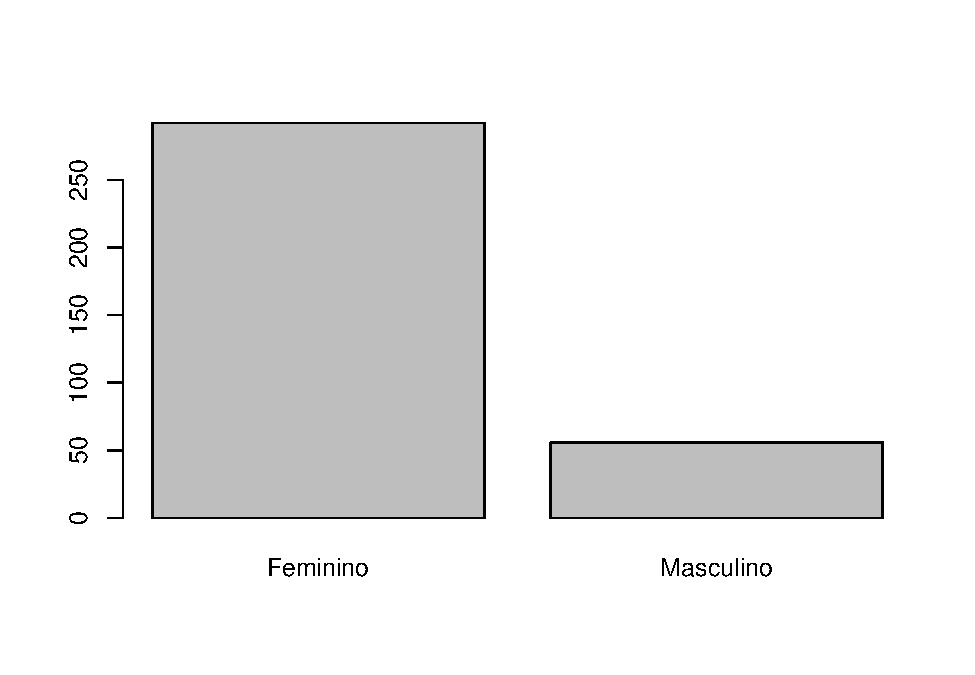
\includegraphics[width=\textwidth]{index_files/figure-latex/unnamed-chunk-67-1} 

}

\caption{Gráfico de colunas com a variável Sexo}\label{fig:unnamed-chunk-67}
\end{figure}

\textbf{Obs}.: É possível personalizar o gráfico, incluindo o título do
eixo x (xlab), o título do eixoy (ylab), o título do gráfico (main), a
cor da coluna (col) e cor da borda da coluna (border), lembrando que as
cores, assim como os comandos devem ser expressas em inglês.

\texttt{barplot(table(nome\_variável),\ col=c("blue","red"),\ main="Título",\ xlab="Variável\ do\ eixo\ x",\ ylab\ =\ "Informação\ que\ consta\ no\ eixo\ y",border="red")}

\textbf{Ex.1)} Construir um gráfico de colunas para a variável
\textbf{Pessoas\_familia}.

\begin{Shaded}
\begin{Highlighting}[]
\KeywordTok{barplot}\NormalTok{(}\KeywordTok{table}\NormalTok{(}\StringTok{`}\DataTypeTok{Pessoas_familia}\StringTok{`}\NormalTok{), }\DataTypeTok{col=}\KeywordTok{c}\NormalTok{(}\StringTok{"blue"}\NormalTok{), }\DataTypeTok{main =} \StringTok{"Frequência de pessoas por família"}\NormalTok{, }\DataTypeTok{xlab =} \StringTok{"Frequência", ylab = "}\NormalTok{Pessoas}\StringTok{", border = "}\NormalTok{red}\StringTok{")}
\end{Highlighting}
\end{Shaded}

\begin{figure}

{\centering 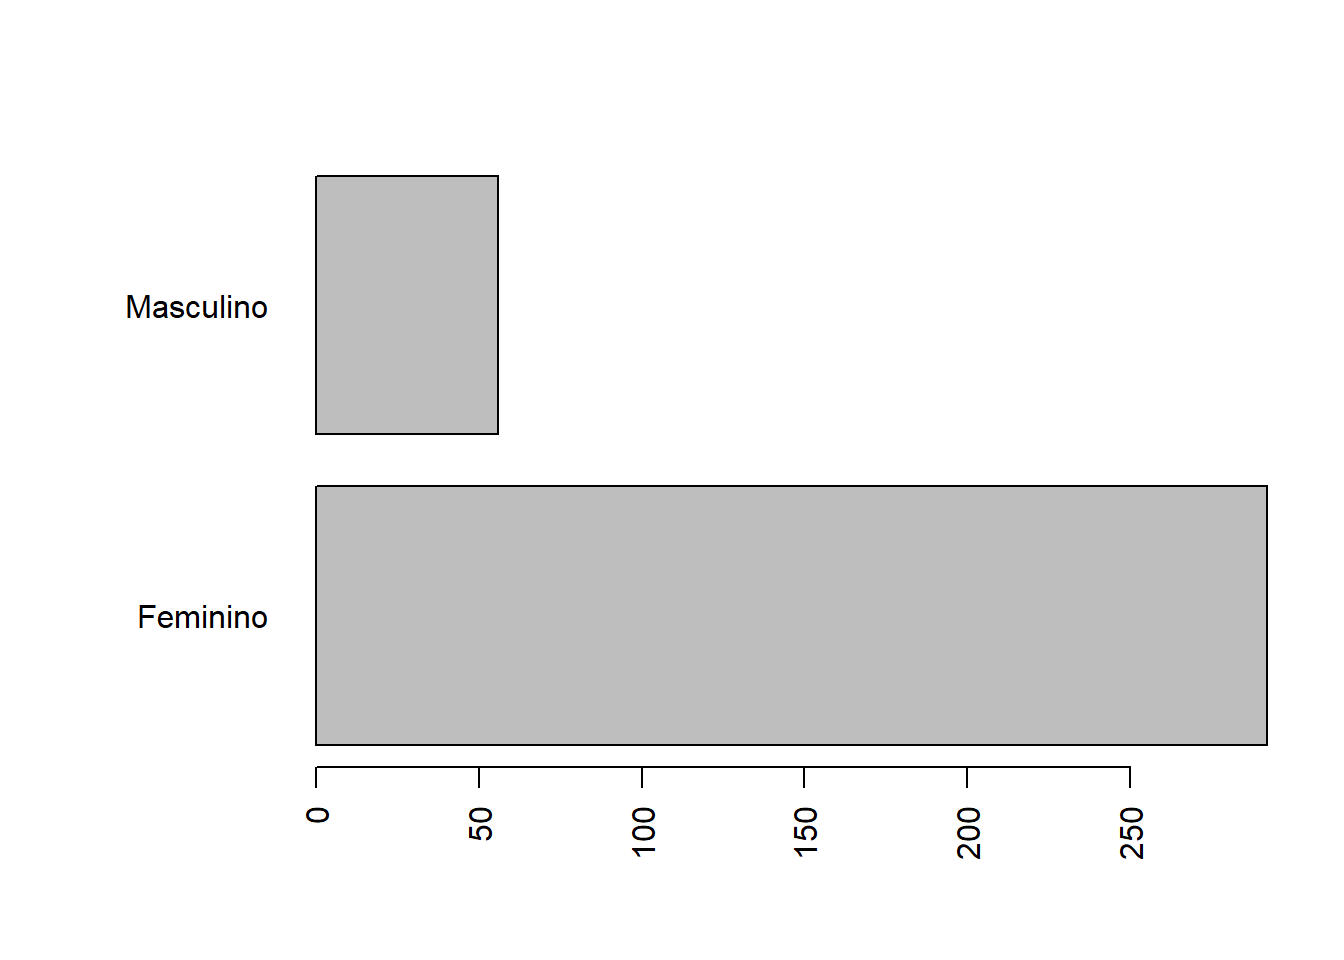
\includegraphics[width=\textwidth]{index_files/figure-latex/unnamed-chunk-68-1} 

}

\caption{Gráfico de colunas com a variável `Pessoas familia`}\label{fig:unnamed-chunk-68}
\end{figure}

\textbf{Ex.2)} Construir uma tabela de dupla entrada para as variáveis
\textbf{Sexo} e \textbf{Divulgação}.

\begin{Shaded}
\begin{Highlighting}[]
\KeywordTok{barplot}\NormalTok{(}\KeywordTok{table}\NormalTok{(Sexo,Divulgacao), }\DataTypeTok{col=}\KeywordTok{c}\NormalTok{(}\StringTok{"blue"}\NormalTok{), }
  \DataTypeTok{main =} \StringTok{"Frequência de pessoas por Sexo e Divulgacao"}\NormalTok{)}
\end{Highlighting}
\end{Shaded}

\begin{figure}

{\centering 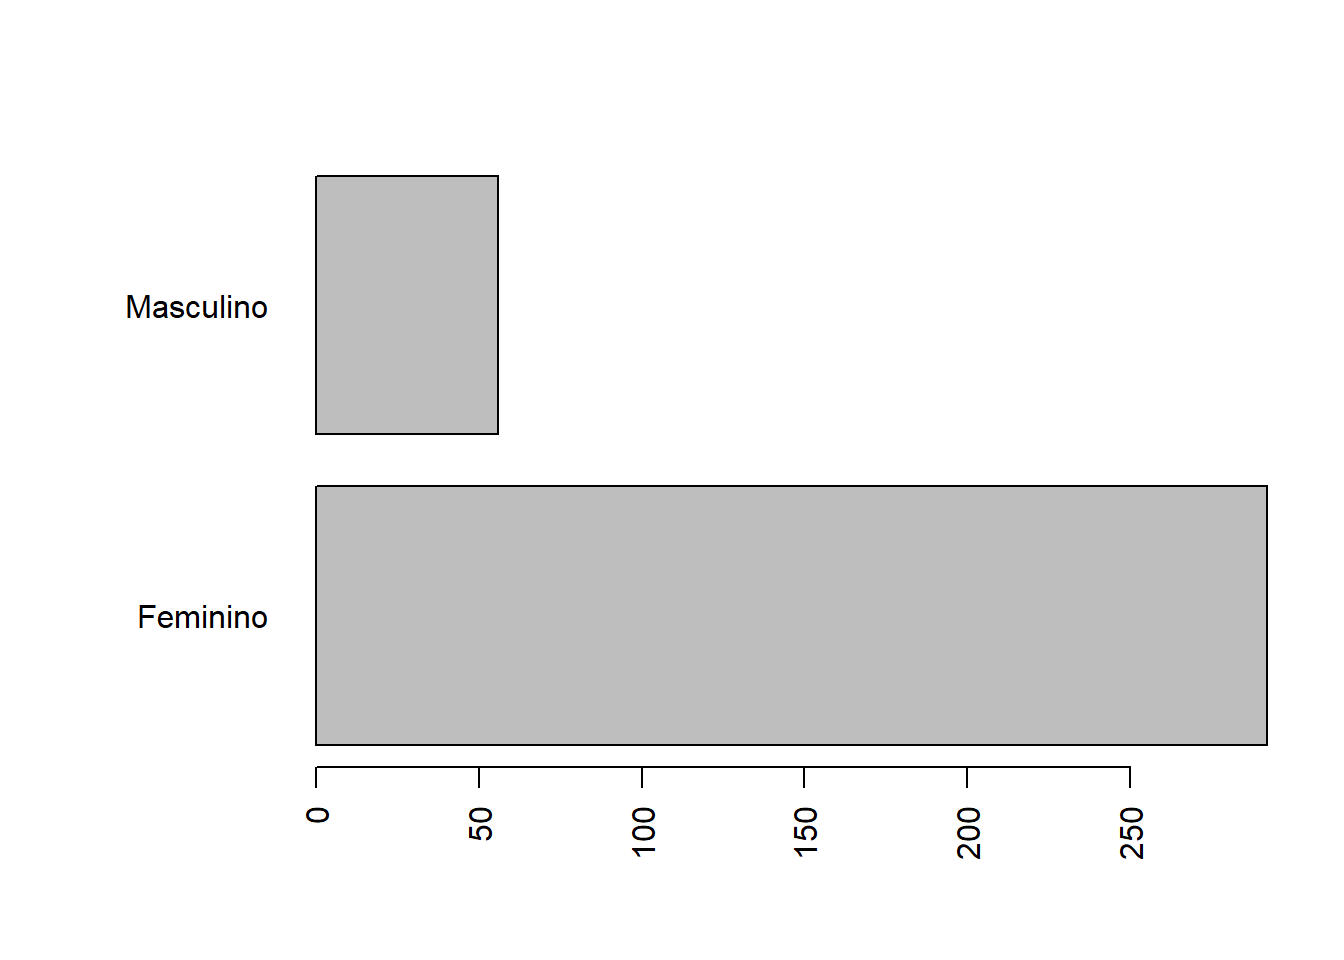
\includegraphics[width=\textwidth]{index_files/figure-latex/unnamed-chunk-69-1} 

}

\caption{Gráfico de colunas com as variáveis Sexo e Divulgacao}\label{fig:unnamed-chunk-69}
\end{figure}

\textbf{Ex.3)} Na sequência utiliza o sinal de atribuição \textless{}-
para atribuir o nome Resultado para esta tabela (tabela de dupla entrada
obtida em Ex.2).

\begin{Shaded}
\begin{Highlighting}[]
\NormalTok{Resultado<-}\KeywordTok{table}\NormalTok{(Sexo,Divulgacao)}
\end{Highlighting}
\end{Shaded}

\textbf{Ex.4)} Execute o seguinte comando:

\begin{Shaded}
\begin{Highlighting}[]
\KeywordTok{barplot}\NormalTok{(Resultado,}\DataTypeTok{col=}\KeywordTok{c}\NormalTok{(}\StringTok{"blue"}\NormalTok{,}\StringTok{"red"}\NormalTok{),}\DataTypeTok{main=}\StringTok{"Título"}\NormalTok{,}\DataTypeTok{xlab=}\StringTok{"Variável do eixo x"}\NormalTok{,}
        \DataTypeTok{ylab=}\StringTok{"Informação que consta no eixo y"}\NormalTok{, }\DataTypeTok{border=}\StringTok{'red'}\NormalTok{, }
        \DataTypeTok{beside=}\NormalTok{T,}\DataTypeTok{legend=}\KeywordTok{rownames}\NormalTok{(Resultado))}
\end{Highlighting}
\end{Shaded}

\begin{figure}

{\centering 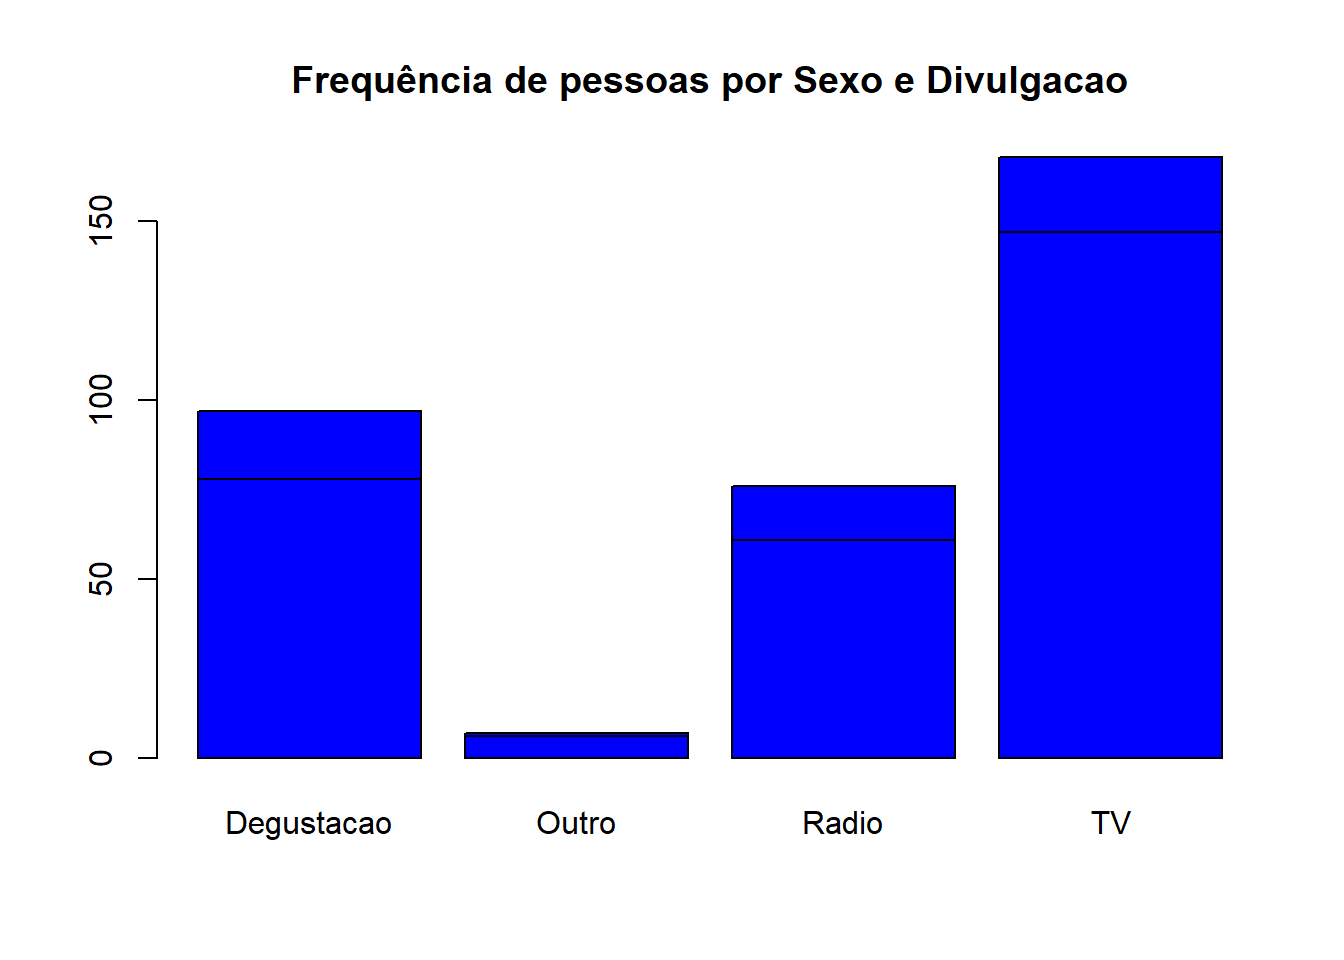
\includegraphics[width=\textwidth]{index_files/figure-latex/unnamed-chunk-71-1} 

}

\caption{Gráfico de colunas com as variáveis Sexo e Divulgacao (2)}\label{fig:unnamed-chunk-71}
\end{figure}

Observe que o uso do argumento \texttt{beside=T} evita que as barras
fiquem empilhadas e o arguemnto \texttt{legend}' insere a legenda
conforme as cores das colunas.

\textbf{Ex.5)} Repita o exercício a partir do Ex.3, invertendo a ordem
entre as variáveis qualitativas.

\hypertarget{setograma-ou-grafico-de-pizza}{%
\subsection{Setograma ou gráfico de
pizza}\label{setograma-ou-grafico-de-pizza}}

Os gráficos em setores são utilizados para ilustrar dados qualitativos
de modo mais compreensível. Quando a variável é ordinal, gráficos de
colunas são mais indicados pelo fato de permitirem manter a ordem das
categorias. Isto também vale para os casos em que se tem muitas
categorias ou quanto se pretende dar mais destaque às categorias mais
frequentes \autocite{barbetta1988}.

\texttt{pie(table(nome\_variável),main="nome")}

Ex. Construa um gráfico na forma de Setograma para a variável
\textbf{Sabor}.

\begin{Shaded}
\begin{Highlighting}[]
\KeywordTok{pie}\NormalTok{(}\KeywordTok{table}\NormalTok{(Sabor))}
\end{Highlighting}
\end{Shaded}

\begin{figure}

{\centering 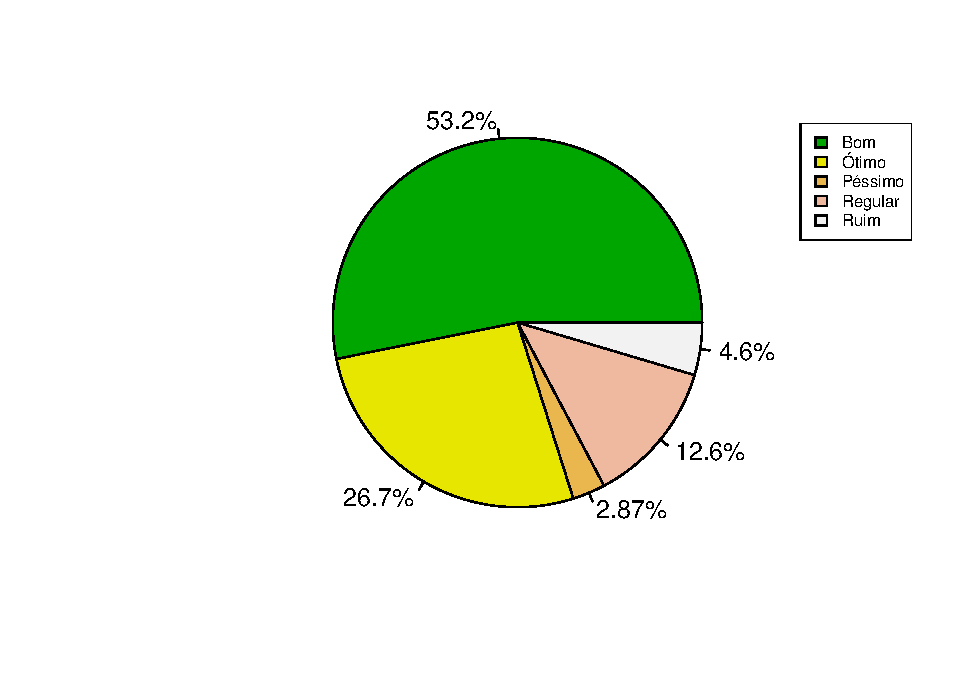
\includegraphics[width=\textwidth]{index_files/figure-latex/unnamed-chunk-72-1} 

}

\caption{Gráfico de pizza com a variável Sabor}\label{fig:unnamed-chunk-72}
\end{figure}

\hypertarget{histograma}{%
\subsection{Histograma}\label{histograma}}

No histograma, utilizado em geral quando temos variáveis quantitativas
contínuas, a altura dos retângulos representa a frequência de ocorrência
de valores no intervalo (deve iniciar sempre em zero), devem ter sempre
a mesma largura podendo ser justapostos. O eixo horizontal (dos valores
da variável) pode iniciar próximo ao menor valor da variável
\autocite{barbetta1988}. Para confecção do histograma devemos usar:

\texttt{hist(nome\_variável)}

Ex. Construa um histograma com a variável \textbf{Renda\_h}.

\begin{Shaded}
\begin{Highlighting}[]
\KeywordTok{hist}\NormalTok{(}\KeywordTok{as.numeric}\NormalTok{(}\StringTok{`}\DataTypeTok{Renda_h}\StringTok{`}\NormalTok{))}
\end{Highlighting}
\end{Shaded}

\begin{figure}

{\centering 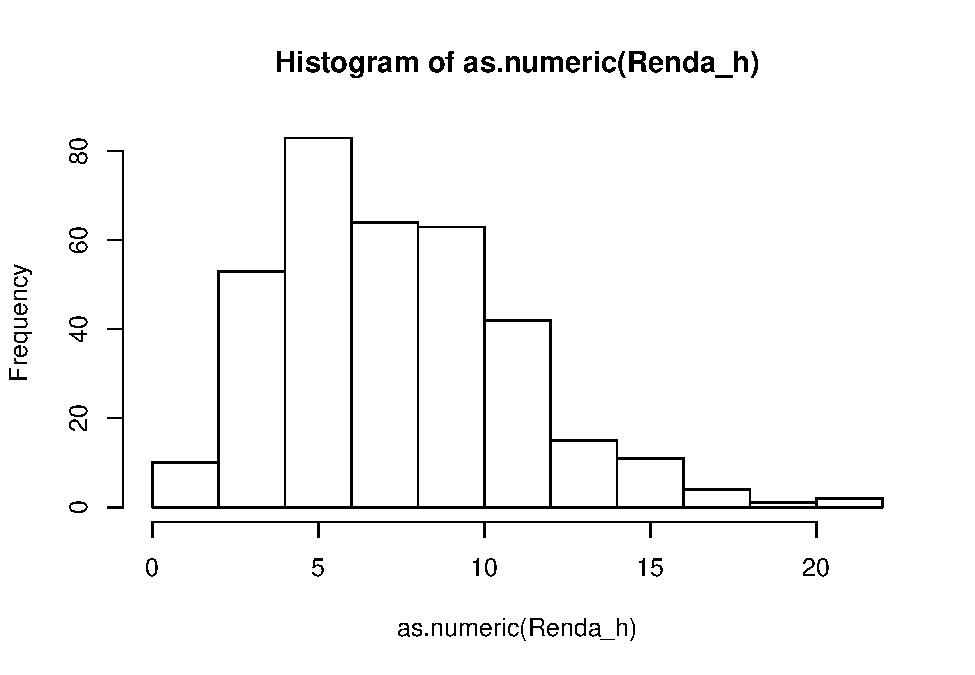
\includegraphics[width=\textwidth]{index_files/figure-latex/unnamed-chunk-73-1} 

}

\caption{Histograma com a variável `Renda h`}\label{fig:unnamed-chunk-73}
\end{figure}

\textbf{Obs}. I: Neste caso também é possível personalizar o gráfico,
incluindo o título do eixo x (xlab), o título do eixoy (ylab), o título
do gráfico (main), a cor da coluna (col) e cor da borda da coluna
(border), lembrando que as cores, assim como os comandos devem ser
expressas em inglês.

\textbf{Obs}. II: Para definir o número de intervalos no Histograma,
usamos:

\texttt{hist(nome\_variável,\ breaks\ =\ 5)}

\begin{Shaded}
\begin{Highlighting}[]
\KeywordTok{hist}\NormalTok{(}\KeywordTok{as.numeric}\NormalTok{(}\StringTok{`}\DataTypeTok{Renda_h}\StringTok{`}\NormalTok{), }\DataTypeTok{breaks=}\DecValTok{5}\NormalTok{)}
\end{Highlighting}
\end{Shaded}

\begin{figure}

{\centering 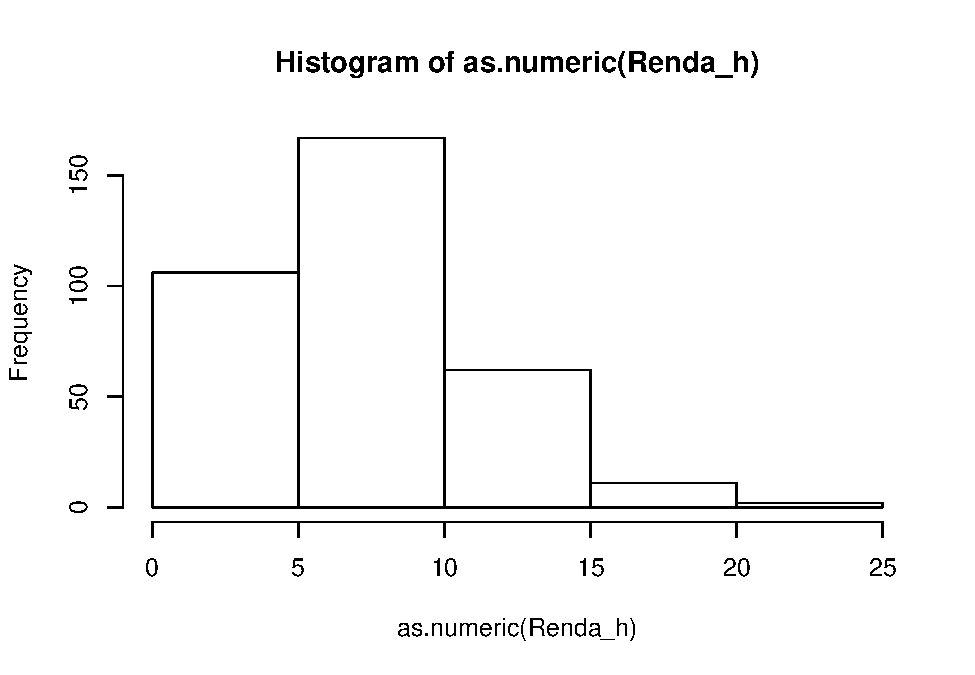
\includegraphics[width=\textwidth]{index_files/figure-latex/unnamed-chunk-74-1} 

}

\caption{Histograma com a variável Renda h com breaks=5}\label{fig:unnamed-chunk-74}
\end{figure}

Use o argumento \texttt{main=NULL} para remover o título.

\hypertarget{boxplot-ou-diagrama-em-caixas}{%
\subsection{Boxplot ou diagrama em
caixas}\label{boxplot-ou-diagrama-em-caixas}}

Os diagramas em caixa são convenientes para revelar tendências centrais,
dispersão, distribuição dos dados e a presença de outliers (valores
extremos). Como as medianas revelam uma tendência central, ao passo que
os quartis indicam a dispersão dos dados, os diagramas em caixa têm a
vantagem de não serem tão sensíveis a valores extremos como outras
medidas baseadas na média e no desvio-padrão. Por outro lado, os
diagramas em caixa (boxplots) não dão informação tão detalhada quanto os
histogramas ou os gráficos ramo-e-folhas, podendo não ser, assim, a
melhor escolha quando lidamos com um único conjunto de dados. Os
diagramas em caixa são, entretanto, mais convenientes na comparação de
dois ou mais conjuntos de dados \autocite{triola1999}.

No diagrama de caixas, torna-se fácil identificar \textbf{outliers} (ou
valores extremos), que são valores extremamente raros, no sentido de que
estão muito afastados da maioria dos dados. Ao explorarmos um conjunto
de dados, não podem deixar de considerar os outliers, porque eles podem
revelar informações importantes \autocite{triola1999}.

Para obter o boxplot para um conjunto de dados:

\texttt{boxplot(variávelA,\ variávelB,\ names=c("A","B"))}

\textbf{Ex.1)} Construir um boxplot da variável \textbf{Idade}.

\begin{Shaded}
\begin{Highlighting}[]
\KeywordTok{boxplot}\NormalTok{(Idade,}\DataTypeTok{horizontal =}\NormalTok{ T)}
\end{Highlighting}
\end{Shaded}

\begin{figure}

{\centering 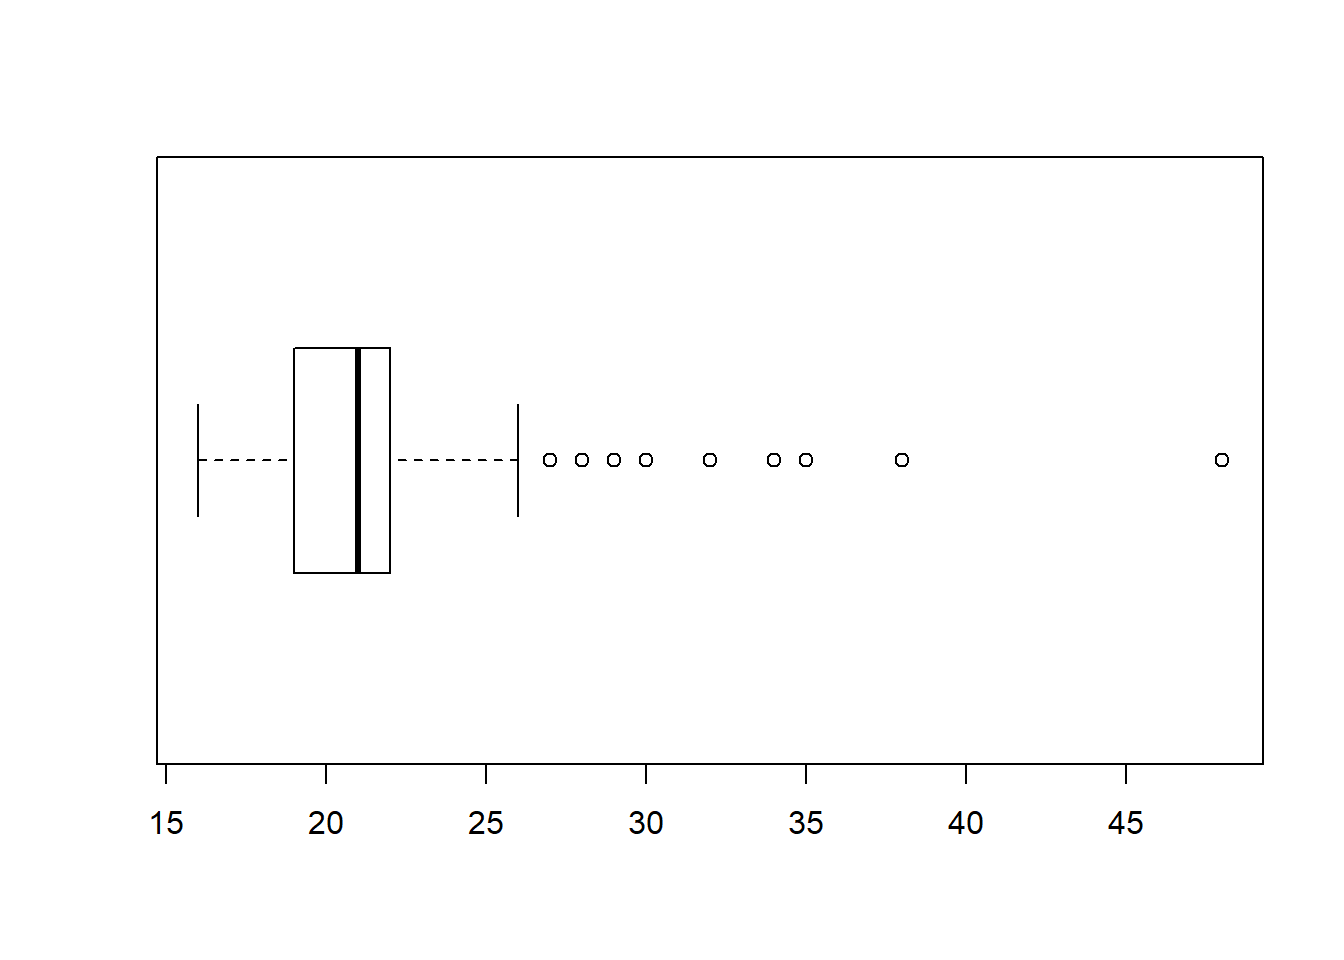
\includegraphics[width=\textwidth]{index_files/figure-latex/unnamed-chunk-75-1} 

}

\caption{Boxplot com a variável Idade}\label{fig:unnamed-chunk-75}
\end{figure}

\textbf{Ex.2)} Construir um boxplot das variáveis \textbf{Peso\_(Kg)} e
\textbf{Altura\_(m)}.

\hypertarget{grafico-ramo-e-folhas}{%
\subsection{Gráfico ramo-e-folhas}\label{grafico-ramo-e-folhas}}

Em um gráfico ramo-e-folhas, classificamos os dados segundo um padrão
que revela a distribuição subjacente. O padrão consiste em separar um
número em duas partes em geral: o ramo consiste nos algarismos mais à
esquerda e as folhas consistem nos algarismos mais à direita.

No gráfico Ramo-e-folhas, podemos ver a distribuição desses dados, que é
uma vantagem do gráfico ramo-e-folhas e ainda conservar toda a
informação da lista original; se necessário, podemos recompor a relação
original de valores. Note que as linhas de algarismos em um gráfico
ramo-e-folhas são análogas, em natureza, às barras de um histograma
\autocite{triola1999}.

\texttt{stem(nome\_variável)} - comando que permite obter um gráfico
Ramo e Folhas.

Ou

\texttt{stem(nome\_variável,scale=1)}

O ``scale=1'', que é o padrão, separa os ramos das folhas a partir das
casas decimais.

Caso padrão:

\begin{itemize}
\tightlist
\item
  A ideia do ramo e folhas é separar um número (como 16,0) em duas
  partes. Assim, a primeira parte inteira (16) chamada de ramo e a
  segunda, a parte decimal (0) chamada de folha. O padrão do R é separar
  os números em duas partes (inteira e decimal) e agrupar os números em
  classes de tamanho 2. Por exemplo, o ramo 16 leva em conta os números
  16 e 17.
\end{itemize}

\textbf{Obs.}: Esse padrão vai se alterando, à medida que o conjunto de
dados apresente diferentes casas decimais.

Assim, outras opções podem ser avaliadas:

\begin{enumerate}
\def\labelenumi{\alph{enumi})}
\item
  \texttt{stem(nome\_variável,scale=0.5)}
\item
  \texttt{stem(nome\_variável,scale=2)}
\end{enumerate}

\textbf{Obs.}: Quando uma folha relacionada com certo ramo tem uma
quantidade tão grande de valores que ele sintetiza essa quantidade
usando a denominação +n, e invade a linha seguinte. Isso pode ser
melhorado usando \textbf{width}.

\begin{enumerate}
\def\labelenumi{\alph{enumi})}
\setcounter{enumi}{2}
\tightlist
\item
  \texttt{stem(nome\_variável,scale=0.5,width=120)}
\end{enumerate}

Ex. Construa um gráfico Ramo e Follhas com a variável \textbf{Idade}.

\begin{Shaded}
\begin{Highlighting}[]
\KeywordTok{stem}\NormalTok{(Idade,}\DataTypeTok{scale=}\DecValTok{2}\NormalTok{)}
\end{Highlighting}
\end{Shaded}

\begin{verbatim}

  The decimal point is at the |

  16 | 000
  17 | 000000000
  18 | 0000000000000000000000000000000000000000
  19 | 000000000000000000000000000000000000000000000000
  20 | 0000000000000000000000000000000000000000000000000000000000000000
  21 | 000000000000000000000000000000000000000000000000000000000000
  22 | 0000000000000000000000000000000000000000000
  23 | 000000000000
  24 | 000000000
  25 | 0000
  26 | 00000000000
  27 | 00000000000
  28 | 0000000000000
  29 | 00
  30 | 00000
  31 | 
  32 | 00
  33 | 
  34 | 00
  35 | 00
  36 | 
  37 | 
  38 | 000
  39 | 
  40 | 
  41 | 
  42 | 
  43 | 
  44 | 
  45 | 
  46 | 
  47 | 
  48 | 00000
\end{verbatim}

\hypertarget{graficos-de-dispersao}{%
\subsection{Gráficos de dispersão}\label{graficos-de-dispersao}}

Às vezes temos dados emparelhados de forma que associa cada valor de um
conjunto a um determinado valor de um segundo conjunto. Um diagrama de
dispersão é um gráfico dos dados emparelhados (x, y), com um eixo x
horizontal e um eixo y vertical. O diagrama de dispersão, apresenta no
eixo horizontal os valores da primeira variável e um eixo vertical para
os valores da segunda variável. O padrão dos pontos assim marcados
costuma ajudar a determinar se existe algum relacionamento entre as duas
variáveis A e B.

\texttt{plot(variável\_independente,Variável\_dependente)}

Ou

\texttt{plot(variável\_dependente\textasciitilde{}variável\_independente)}

\hypertarget{grafico-de-linhas}{%
\subsection{Gráfico de linhas}\label{grafico-de-linhas}}

Apresenta a evolução de um dado, geralmente ao longo do tempo. Eixos na
vertical e na horizontal indicam as informações a que se refere e a
linha traçada entre eles, ascendente, descendente constante ou com
vários altos e baixos mostra o percurso de um fenômeno específico.

Ex. Considere os dados que descrevem os valores do número de empresas
fiscalizadas na fiscalização do trabalho na área rural Brasil 1998-2010.

\begin{table}

\caption{\label{tab:unnamed-chunk-77}Evolução dos resultados da fiscalização do trabalho na área rural Brasil 1998-2010}
\centering
\begin{tabular}[t]{r|l}
\hline
Ano & Empresas.Fiscalizadas\\
\hline
1998 & 7.042\\
\hline
1999 & 6.561\\
\hline
2000 & 8.585\\
\hline
2001 & 9.641\\
\hline
2002 & 8.873\\
\hline
2003 & 9.367\\
\hline
2004 & 13.856\\
\hline
2005 & 12.192\\
\hline
2006 & 13.326\\
\hline
2007 & 13.390\\
\hline
2008 & 10.839\\
\hline
2009 & 13.379\\
\hline
2010 & 11.978\\
\hline
\end{tabular}
\end{table}

Para construir um gráfico de linhas, utilizamos o seguinte comando:

\texttt{plot(x,y,type=\ "Tipo\ de\ símbolo")}

Neste gráfico, podemos utilizar comandos já utilizados anteriormente,
para inserir título, nomes dos eixos, etc. Para escolher o formato das
linhas, com o uso do argumento ```type''\textbar{}, seguem algumas
opções:

\begin{itemize}
\tightlist
\item
  \texttt{"p"} para pontos,
\item
  \texttt{"l"} para linhas,
\item
  \texttt{"b"} para pontos e linhas,
\item
  \texttt{"c"} para linhas descontínuas nos pontos,
\item
  \texttt{"o"} para pontos sobre as linhas,
\item
  \texttt{"n"} para nenhum gráfico, apenas a janela.
\end{itemize}

Para o caso de representação no mesmo gráfico, de duas ou mais
variáveis, o processo deverá ser realizado por etapas:

\texttt{plot(x,y1,type="b",main="Título",\ xlab="Nome\_eixo\_x",ylab="Nome\_eixo\_y",\ col="cor\ das\ linhas",ylim=c(yi,ys))}

\begin{Shaded}
\begin{Highlighting}[]
\NormalTok{empfisc=}\KeywordTok{data.frame}\NormalTok{(}\DataTypeTok{ano=}\KeywordTok{c}\NormalTok{(}\DecValTok{1998}\NormalTok{,}\DecValTok{1999}\NormalTok{,}\DecValTok{2000}\NormalTok{,}\DecValTok{2001}\NormalTok{,}\DecValTok{2002}\NormalTok{,}\DecValTok{2003}\NormalTok{,}\DecValTok{2004}\NormalTok{,}\DecValTok{2005}\NormalTok{,}\DecValTok{2006}\NormalTok{,}\DecValTok{2007}\NormalTok{,}
    \DecValTok{2008}\NormalTok{,}\DecValTok{2009}\NormalTok{,}\DecValTok{2010}\NormalTok{), }\DataTypeTok{qtd=}\KeywordTok{c}\NormalTok{(}\DecValTok{7042}\NormalTok{,}\DecValTok{6561}\NormalTok{,}\DecValTok{8585}\NormalTok{,}\DecValTok{9641}\NormalTok{,}\DecValTok{8873}\NormalTok{,}\DecValTok{9367}\NormalTok{,}
\DecValTok{13856}\NormalTok{,}\DecValTok{12192}\NormalTok{,}\DecValTok{13326}\NormalTok{,}\DecValTok{13390}\NormalTok{,}\DecValTok{10839}\NormalTok{,}\DecValTok{13379}\NormalTok{,}\DecValTok{11978}\NormalTok{))}

\KeywordTok{plot}\NormalTok{(empfisc}\OperatorTok{$}\NormalTok{ano,empfisc}\OperatorTok{$}\NormalTok{qtd,}\DataTypeTok{type=}\StringTok{"b"}\NormalTok{,}\DataTypeTok{main=}\StringTok{"Título"}\NormalTok{,}
     \DataTypeTok{xlab=}\StringTok{"Nome_eixo_x"}\NormalTok{,}\DataTypeTok{ylab=}\StringTok{"Nome_eixo_y"}\NormalTok{, }
     \DataTypeTok{col=}\StringTok{"blue"}\NormalTok{,}\DataTypeTok{xlim=}\KeywordTok{c}\NormalTok{(}\DecValTok{1998}\NormalTok{,}\DecValTok{2010}\NormalTok{))}
\end{Highlighting}
\end{Shaded}

\begin{figure}

{\centering 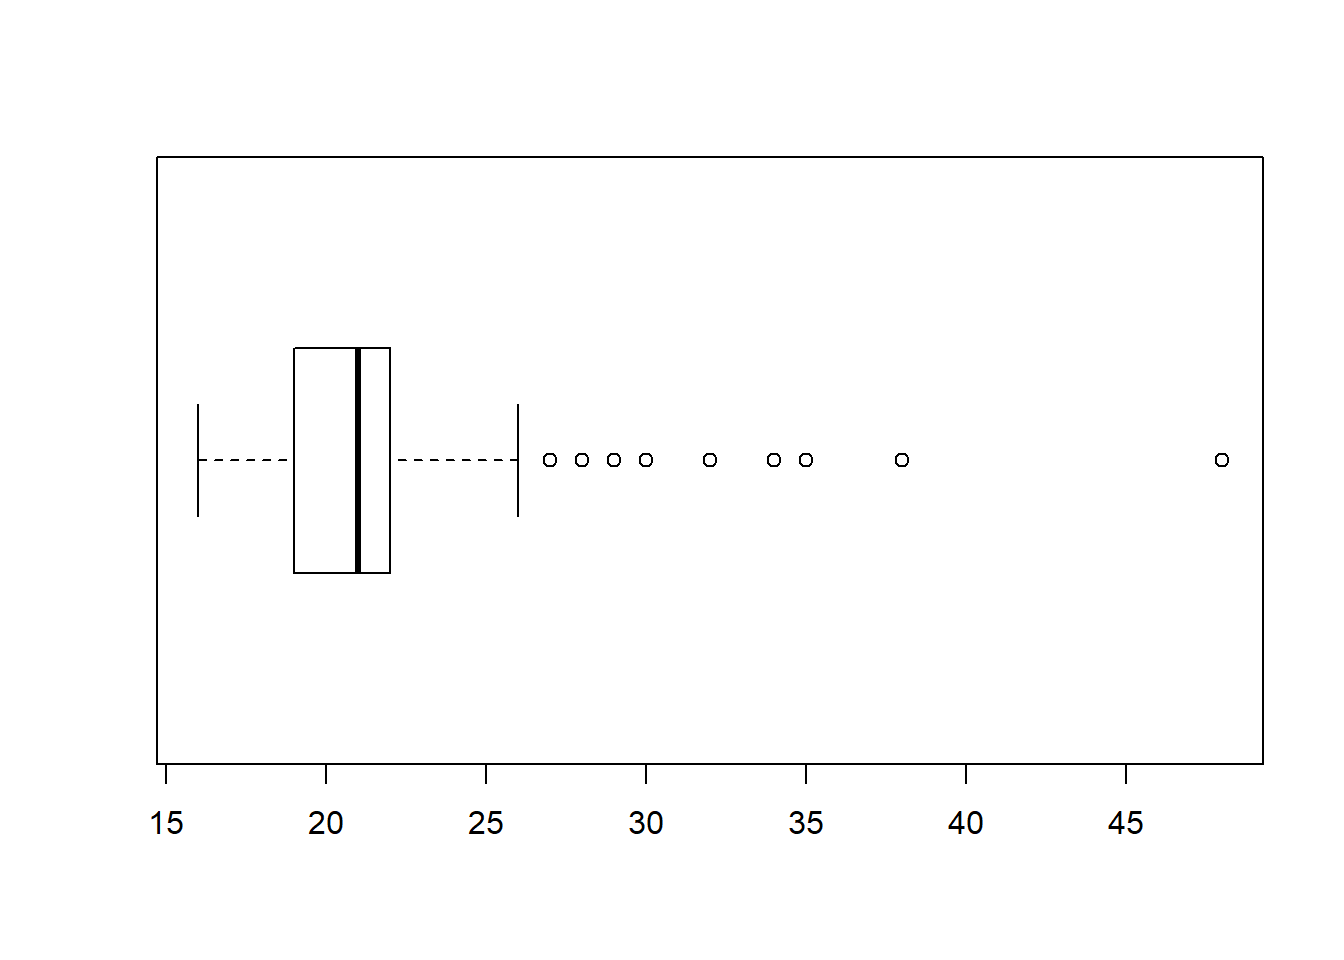
\includegraphics[width=\textwidth]{index_files/figure-latex/unnamed-chunk-78-1} 

}

\caption{Gráfico de linha sobre a fiscalização do trabalho na área rural Brasil 1998-2010}\label{fig:unnamed-chunk-78}
\end{figure}

onde, no argumento \texttt{ylim}, devemos indicar o intervalo de
variação dos valores de y, ou seja todo o intervalo que será necessário
para representar todas as variáveis.

Na sequência adicionamos as instruções para as demais variáveis:

\texttt{lines(x,\ y2,col="cor\_desejada",\ type="b")}

Com o argumento \texttt{"legend"} instruímos a formatação da legenda:

\texttt{legend(xp,yp,c("representação\_variável\_1\ na\ legenda",\ "representação\_variável\_2\ na\ legenda"),}col
=c(``Cor1'',``cor2''),pch=Valor entre 0 e 25)`

Obs.: \texttt{pch}= número (entre 0 e 25). No Help do R (buscando com
pch), você encontra a lista completa de símbolos que podem ser
utilizados na representação da legenda. Neste caso, pode ser importante
também alterar o tamanho da fonte da legenda, com o uso do argumento
\texttt{"cex"}.

Exemplo: Segue exemplo de um gráfico de linhas para as temperaturas
registradas durante o dia 11/04/2018, pela Estação Meteorológica de São
Luiz Gonzaga, RS, conforme dados obtidos no site do Inmet.

\begin{Shaded}
\begin{Highlighting}[]
\KeywordTok{library}\NormalTok{(readr)}
\NormalTok{inmet <-}\StringTok{ }\KeywordTok{read_delim}\NormalTok{(}\StringTok{"https://goo.gl/se71v2"}\NormalTok{, }
    \StringTok{";"}\NormalTok{, }\DataTypeTok{escape_double =} \OtherTok{FALSE}\NormalTok{, }
    \DataTypeTok{col_types =} \KeywordTok{cols}\NormalTok{(}\DataTypeTok{data =} \KeywordTok{col_date}\NormalTok{(}\DataTypeTok{format =} \StringTok{"%m/%d/%Y"}\NormalTok{)), }
    \DataTypeTok{trim_ws =} \OtherTok{TRUE}\NormalTok{)}
\KeywordTok{head}\NormalTok{(inmet)}
\end{Highlighting}
\end{Shaded}

\begin{verbatim}
# A tibble: 6 x 6
  codigo_estacao data        hora temp_inst temp_max temp_min
  <chr>          <date>     <int>     <dbl>    <dbl>    <dbl>
1 A852           2018-04-11     0      26.2     27.1     26.2
2 A852           2018-04-11     1      26       26.2     26  
3 A852           2018-04-11     2      25.5     26.1     25.5
4 A852           2018-04-11     3      25.1     25.5     25  
5 A852           2018-04-11     4      24.6     25.2     24.5
6 A852           2018-04-11     5      24.3     24.7     24.2
\end{verbatim}

Segue a sequência de comandos, para obtenção do gráfico de linhas:

\begin{Shaded}
\begin{Highlighting}[]
\KeywordTok{plot}\NormalTok{(inmet}\OperatorTok{$}\NormalTok{hora,inmet}\OperatorTok{$}\NormalTok{temp_inst,}\DataTypeTok{type =} \StringTok{"b"}\NormalTok{, }
  \DataTypeTok{main =} \StringTok{"Temperaturas registradas na estação metereológica}
\StringTok{  de São Luis Gonzaga, 11 de abril de 2018"}\NormalTok{,}
  \DataTypeTok{xlab =} \StringTok{"hora"}\NormalTok{,}\DataTypeTok{ylab =} \StringTok{"temperaturas"}\NormalTok{,}\DataTypeTok{col=}\StringTok{"blue"}\NormalTok{,}
  \DataTypeTok{ylim =} \KeywordTok{c}\NormalTok{(}\DecValTok{20}\NormalTok{,}\DecValTok{40}\NormalTok{))}

\KeywordTok{lines}\NormalTok{(inmet}\OperatorTok{$}\NormalTok{hora,inmet}\OperatorTok{$}\NormalTok{temp_max,}\DataTypeTok{col=}\StringTok{"red"}\NormalTok{,}\DataTypeTok{type =} \StringTok{"b"}\NormalTok{)}

\KeywordTok{lines}\NormalTok{(inmet}\OperatorTok{$}\NormalTok{hora,inmet}\OperatorTok{$}\NormalTok{temp_min,}\DataTypeTok{col=}\StringTok{"green"}\NormalTok{,}\DataTypeTok{type =} \StringTok{"b"}\NormalTok{)}

\KeywordTok{legend}\NormalTok{(}\DecValTok{0}\NormalTok{,}\DecValTok{40}\NormalTok{,}\KeywordTok{c}\NormalTok{(}\StringTok{"temp_inst"}\NormalTok{,}\StringTok{"temp_max"}\NormalTok{,}\StringTok{"temp_min"}\NormalTok{),}
  \DataTypeTok{col =}\KeywordTok{c}\NormalTok{(}\StringTok{"blue"}\NormalTok{,}\StringTok{"red"}\NormalTok{,}\StringTok{"green"}\NormalTok{),}\DataTypeTok{pch=}\FloatTok{4.1}\NormalTok{,}\DataTypeTok{cex =} \FloatTok{0.75}\NormalTok{)}
\end{Highlighting}
\end{Shaded}

\begin{figure}

{\centering 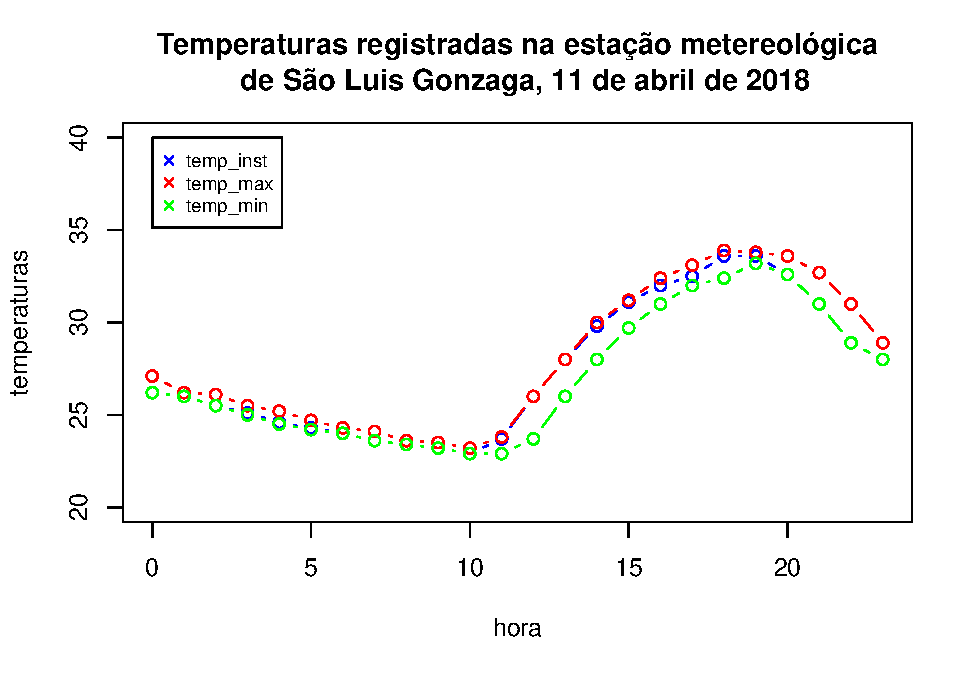
\includegraphics[width=\textwidth]{index_files/figure-latex/unnamed-chunk-80-1} 

}

\caption{Gráfico de linha sobre as temperaturas registradas em São Luiz Gonzaga - RS}\label{fig:unnamed-chunk-80}
\end{figure}

\hypertarget{estatisticas-descritivas}{%
\section{Estatísticas Descritivas}\label{estatisticas-descritivas}}

Para determinar o valor máximo de um conjunto de dados, utilizamos:

\texttt{max(nome\_da\_variável)}

Use a variável \textbf{Renda\_h}

\begin{Shaded}
\begin{Highlighting}[]
\CommentTok{#Transforme a variável Renda_h em variável numérica}
\NormalTok{pesquisa_dados}\OperatorTok{$}\NormalTok{Renda_h=}\KeywordTok{as.numeric}\NormalTok{(pesquisa_dados}\OperatorTok{$}\NormalTok{Renda_h)}
\CommentTok{#É preciso repetir o comando attach()}
\KeywordTok{attach}\NormalTok{(pesquisa_dados)}
\KeywordTok{max}\NormalTok{(Renda_h)}
\end{Highlighting}
\end{Shaded}

\begin{verbatim}
[1] 21.83
\end{verbatim}

De forma análoga, para determinar o valor mínimo de um conjunto de
dados, utilizamos:

\texttt{min(nome\_da\_variável)}

Use a variável \textbf{Renda\_h}

\begin{verbatim}
min(Renda_h)
\end{verbatim}

\textbf{Obs.}: Para determinar a amplitude total de um conjunto de
dados, utilizamos:

\texttt{max(nome\_da\_variável)-min(nome\_da\_variável)}

Use a variável \textbf{Renda\_h}

\begin{Shaded}
\begin{Highlighting}[]
\KeywordTok{max}\NormalTok{(Renda_h)}\OperatorTok{-}\KeywordTok{min}\NormalTok{(Renda_h)}
\end{Highlighting}
\end{Shaded}

\begin{verbatim}
[1] 20.81
\end{verbatim}

Para obter as medidas da estatística descritiva, no caso medidas de
tendência central (mínimo, quartil 1, mediana, média, quartil 3,
máximo):

\texttt{summary(nome\_da\_variável)}

Ex. Use a variável \textbf{Renda\_h}

\begin{Shaded}
\begin{Highlighting}[]
\KeywordTok{summary}\NormalTok{(Renda_h)}
\end{Highlighting}
\end{Shaded}

\begin{verbatim}
   Min. 1st Qu.  Median    Mean 3rd Qu.    Max. 
   1.02    4.64    6.79    7.31    9.51   21.83 
\end{verbatim}

A moda é o valor que tem o maior número de ocorrências em um conjunto de
dados.

O R não tem um padrão de função embutida para calcular a moda. Uma
sugestão é a criação de uma função pelo usuário, que pode ser obtida,
por exemplo por:

\texttt{subset(table(variável),\ table(variável)==max(table(variável)))}

Ex. Use a variável \textbf{Praticidade}

\begin{Shaded}
\begin{Highlighting}[]
\KeywordTok{subset}\NormalTok{(}\KeywordTok{table}\NormalTok{(Praticidade), }
       \KeywordTok{table}\NormalTok{(Praticidade)}\OperatorTok{==}\KeywordTok{max}\NormalTok{(}\KeywordTok{table}\NormalTok{(Praticidade)))}
\end{Highlighting}
\end{Shaded}

\begin{verbatim}
Ruim 
  95 
\end{verbatim}

Ex. Use a variável quantitativa \textbf{Pessoas\_familia}

\begin{Shaded}
\begin{Highlighting}[]
\KeywordTok{table}\NormalTok{(Pessoas_familia)}
\end{Highlighting}
\end{Shaded}

\begin{verbatim}
Pessoas_familia
 0  1  2  3  4  5  6  7  8  9 10 
 2 14 25 62 73 60 64 30 15  2  1 
\end{verbatim}

\textbf{Obs.}: O primeiro valor encontrado, refere-se ao valor da moda
ao passo que o segundo valor representa quantas vezes esse valor foi
verificado.

Comando que permite determinar o percentil, no caso o percentil 10:

\texttt{quantile(nome\_variável,0.1)}

\textbf{Obs.}: Experimente usar o comando:

\texttt{quantile(nome\_variável)}

\textbf{Obs.}: Para a obtenção de quartis e decis, basta realizar a
conversão para o respectivo percentil e assim calcular normalmente.

\begin{Shaded}
\begin{Highlighting}[]
\KeywordTok{quantile}\NormalTok{(Renda_h)}
\end{Highlighting}
\end{Shaded}

\begin{verbatim}
    0%    25%    50%    75%   100% 
 1.020  4.638  6.785  9.512 21.830 
\end{verbatim}

\begin{Shaded}
\begin{Highlighting}[]
\KeywordTok{quantile}\NormalTok{(Renda_h,}\FloatTok{0.1}\NormalTok{)}
\end{Highlighting}
\end{Shaded}

\begin{verbatim}
  10% 
3.244 
\end{verbatim}

Para obter as medidas de variabilidade, no caso, variância e
desvio-padrão, respectivamente:

\texttt{var(nome\_variável)}

\texttt{sd(nome\_variável)}

Ex. Calcule as medidas de variabilidade com a variável
\textbf{Pessoas\_familia}

\begin{Shaded}
\begin{Highlighting}[]
\KeywordTok{var}\NormalTok{(Pessoas_familia)}
\end{Highlighting}
\end{Shaded}

\begin{verbatim}
[1] 3.245
\end{verbatim}

\begin{Shaded}
\begin{Highlighting}[]
\KeywordTok{sd}\NormalTok{(Pessoas_familia)}
\end{Highlighting}
\end{Shaded}

\begin{verbatim}
[1] 1.801
\end{verbatim}

A função \texttt{subset()}:

Com esta função podemos fazer cálculos utilizando filtros,
simultaneamente. A aplicação de filtros é extremamente útil quando
queremos explorar os dados de forma rápida e eficiente.

Exemplos:

Ex. 1) Altura das pessoas do sexo masculino: com a função abaixo o R
gera um subconjunto com as alturas de todas as pessoas do sexo
masculino.

\begin{Shaded}
\begin{Highlighting}[]
\KeywordTok{subset}\NormalTok{(}\StringTok{`}\DataTypeTok{Altura_(m)}\StringTok{`}\NormalTok{, Sexo}\OperatorTok{==}\StringTok{"Masculino"}\NormalTok{)}
\end{Highlighting}
\end{Shaded}

\begin{verbatim}
 [1] 1.90 1.76 1.83 1.81 1.67 1.55 1.60 1.84 1.80 1.60 1.75 1.73 1.68 1.81 1.90
[16] 1.80 1.56 1.65 1.60 1.61 1.59 1.75 1.59 1.89 1.62 1.60 1.50 1.65 1.79 1.65
[31] 1.79 1.67 1.59 1.71 1.60 1.72 1.73 1.65 1.65 1.50 1.57 1.86 1.85 1.80 1.77
[46] 1.81 1.73 1.80 1.66 1.71 1.60 1.72 1.81 1.55 1.60 1.80
\end{verbatim}

Ex. 2) Média das alturas das pessoas do sexo masculino: inserindo o
comando \texttt{mean()} ao subconjunto anterior, teremos como resultado
a média das alturas das pessoas do sexo masculino.

\begin{Shaded}
\begin{Highlighting}[]
\KeywordTok{mean}\NormalTok{(}\KeywordTok{subset}\NormalTok{(}\StringTok{`}\DataTypeTok{Altura_(m)}\StringTok{`}\NormalTok{, Sexo}\OperatorTok{==}\StringTok{"Masculino"}\NormalTok{))}
\end{Highlighting}
\end{Shaded}

\begin{verbatim}
[1] 1.702
\end{verbatim}

Ex. 3) Média das alturas das pessoas do sexo masculino com mais de 26
anos:

\begin{Shaded}
\begin{Highlighting}[]
\KeywordTok{mean}\NormalTok{(}\KeywordTok{subset}\NormalTok{(}\StringTok{`}\DataTypeTok{Altura_(m)}\StringTok{`}\NormalTok{, Sexo}\OperatorTok{==}\StringTok{"Masculino"}\OperatorTok{&}\StringTok{ }\NormalTok{Idade}\OperatorTok{>}\DecValTok{25}\NormalTok{))}
\end{Highlighting}
\end{Shaded}

\begin{verbatim}
[1] 1.654
\end{verbatim}

Ex. 4) Contagem de pessoas do sexo feminino que tenham menos de 60 kg:

\begin{Shaded}
\begin{Highlighting}[]
\KeywordTok{length}\NormalTok{(}\KeywordTok{subset}\NormalTok{(Sexo,Sexo}\OperatorTok{==}\StringTok{"Feminino"} \OperatorTok{&}\StringTok{ `}\DataTypeTok{Peso_(Kg)}\StringTok{`}\OperatorTok{<}\DecValTok{60}\NormalTok{))}
\end{Highlighting}
\end{Shaded}

\begin{verbatim}
[1] 94
\end{verbatim}

Ex. 5) Montando uma tabela para exibir o gênero de pessoas que
classificaram o Sabor como ``Pessimo'':

\begin{Shaded}
\begin{Highlighting}[]
\KeywordTok{table}\NormalTok{(}\KeywordTok{subset}\NormalTok{(Sexo, Sabor}\OperatorTok{==}\StringTok{"Pessimo"}\NormalTok{))}
\end{Highlighting}
\end{Shaded}

\begin{verbatim}

 Feminino Masculino 
        7         3 
\end{verbatim}

Este capítulo não teve a pretensão de esgotar o estudo de todos os
comandos a serem aplicados na estatística descritiva (veja help do R),
nem tampouco os conceitos estatísticos necessários à compreensão. Para
mais detalhes sobre os conceitos de estatística descritiva, você pode
consultar outras referências ou até mesmo as já citadas neste capítulo.

\hypertarget{inf}{%
\chapter{Estatística Inferencial}\label{inf}}

A inferência estatística, ou estatística inferencial, tem por objetivo
concluir e tomar decisões, com base em amostras (Figura
\ref{fig:infestat}). Usam-se dados extraídos de uma amostra para
produzir inferência sobre a população \autocite{lopes2008}.

\begin{figure}

{\centering 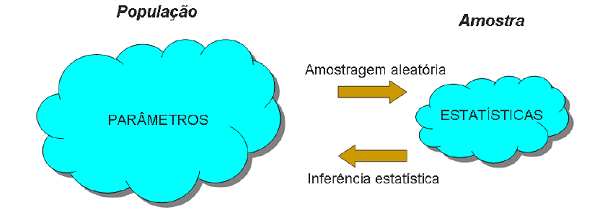
\includegraphics[width=\textwidth]{infestat} 

}

\caption{Inferência Estatística}\label{fig:infestat}
\end{figure}

Em Estatística, o termo \textbf{população} é definido como conjunto de
indivíduos, ou itens, com pelo menos uma característica em comum,
podendo ser finita ou infinita \autocite{lopes2008}. Por exemplo, água
de um rio, sangue de uma pessoa, lote de peças produzidas por uma
indústria, eleitores de um município.

A \textbf{amostra} é um subconjunto, necessariamente finito, de uma
população e é selecionada de forma que todos os elementos da população
tenham a mesma chance de serem escolhidos.

\hypertarget{intervalo-de-confianca}{%
\section{Intervalo de Confiança}\label{intervalo-de-confianca}}

Entre as diferentes técnicas de Inferência Estatística, temos a
Estimação de Parâmetros, que consiste na determinação de um
\textbf{Intervalo de Confiança (IC)} para uma média ou proporção
populacional, ao um nível (1 - \(\alpha\))\% de confiança.

O nível de confiança (1 - \(\alpha\))\% normalmente varia de 90\% a
99\%.

\hypertarget{intervalo-de-confianca-para-uma-media-populacional}{%
\subsection{Intervalo de confiança para uma média
populacional}\label{intervalo-de-confianca-para-uma-media-populacional}}

Um \textbf{intervalo de confiança (IC)} é o \textbf{intervalo} estimado
onde a média de um parâmetro tem uma dada probabilidade de ocorrer.
Comumente define-se como o \textbf{intervalo} onde há (1 - \(\alpha\))\%
de probabilidade da média verdadeira da população inteira ocorrer.

IC (limite inferior \(\leq\) \(\mu\) \(\leq\) limite superior) = (1 -
\(\alpha\))\%

No software RStudio, o Intervalo de Confiança pode ser obtido usando o
teste t.

\textbf{Exemplo 1}: Os dados amostrais a seguir representam o número de
horas de estudos semanais para a disciplina de Estatística Básica, de
uma amostra de 10 alunos:

19 18 20 16 18 19 19 17 22 21

Qual é o intervalo de confiança para a média populacional de onde essa
amostra foi retirada?

\begin{Shaded}
\begin{Highlighting}[]
\NormalTok{horasestudo=}\KeywordTok{c}\NormalTok{(}\DecValTok{19}\NormalTok{,}\DecValTok{18}\NormalTok{,}\DecValTok{20}\NormalTok{,}\DecValTok{16}\NormalTok{,}\DecValTok{18}\NormalTok{,}\DecValTok{19}\NormalTok{,}\DecValTok{19}\NormalTok{,}\DecValTok{17}\NormalTok{,}\DecValTok{22}\NormalTok{,}\DecValTok{21}\NormalTok{)}
\KeywordTok{t.test}\NormalTok{(horasestudo)}
\end{Highlighting}
\end{Shaded}

\begin{verbatim}

    One Sample t-test

data:  horasestudo
t = 33, df = 9, p-value = 1e-10
alternative hypothesis: true mean is not equal to 0
95 percent confidence interval:
 17.62 20.18
sample estimates:
mean of x 
     18.9 
\end{verbatim}

IC (17,6 \(\leq\) \(\mu\) \(\leq\) 20,2) = 95\%

Com 95\% de confiança, a média populacional das horas semanais de estudo
para a disciplina de Estatística Básica está entre 17,6 e 20,2 horas. Ou
seja, qualquer aluno (de onde essa amostra foi retirada) estuda em
média, de 17,6 a 20,2 horas por semana.

Se não informarmos o nível de confiança, o software R considera 95\%. No
entanto, para mudar o nível de confiança para 90\%, acrescentamos a
informação \texttt{conf.level\ =\ 0.90} após o nome da variável:

\begin{Shaded}
\begin{Highlighting}[]
\KeywordTok{t.test}\NormalTok{(horasestudo, }\DataTypeTok{conf.level =} \FloatTok{0.90}\NormalTok{)}
\end{Highlighting}
\end{Shaded}

\begin{verbatim}

    One Sample t-test

data:  horasestudo
t = 33, df = 9, p-value = 1e-10
alternative hypothesis: true mean is not equal to 0
90 percent confidence interval:
 17.86 19.94
sample estimates:
mean of x 
     18.9 
\end{verbatim}

IC (17,9 \(\leq\) \(\mu\) \(\leq\) 19,9) = 90\%

Com 90\% de confiança, a média populacional das horas semanais de estudo
para a disciplina de Estatística Básica está entre 17,9 e 19,9 horas. Ou
seja, qualquer aluno (de onde essa amostra foi retirada) estuda em
média, de 17,9 a 19,9 horas por semana.

Para mudar o nível de confiança para 99\%:

\begin{Shaded}
\begin{Highlighting}[]
\KeywordTok{t.test}\NormalTok{(horasestudo, }\DataTypeTok{conf.level =} \FloatTok{0.99}\NormalTok{)}
\end{Highlighting}
\end{Shaded}

\begin{verbatim}

    One Sample t-test

data:  horasestudo
t = 33, df = 9, p-value = 1e-10
alternative hypothesis: true mean is not equal to 0
99 percent confidence interval:
 17.06 20.74
sample estimates:
mean of x 
     18.9 
\end{verbatim}

IC (17,1 \(\leq\) \(\mu\) \(\leq\) 20,7) = 99\%

Com 99\% de confiança, a média populacional das horas semanais de estudo
para a disciplina de Estatística Básica está entre 17,1 e 20,7 horas. Ou
seja, qualquer aluno (de onde essa amostra foi retirada) estuda em
média, de 17,1 a 20,7 horas por semana.

\hypertarget{para-verificar-normalidade-dos-dados}{%
\subsection{Para verificar normalidade dos
dados}\label{para-verificar-normalidade-dos-dados}}

Algumas técnicas de inferência estatística têm como requisitos a
normalidade dos dados. Para verificar se os dados seguem uma
distribuição normal, podemos, inicialmente usar o histograma e depois
confirmar com um teste estatístico para testar normalidade como
Shapiro-Wilk ou Kolmogorov-Smirnov.

Hipóteses do teste:

\begin{itemize}
\tightlist
\item
  \textbf{H0}: os dados seguem uma distribuição normal
\item
  \textbf{H1}: os dados não seguem uma distribuição normal
\end{itemize}

O \textbf{valor p} reflete a plausibilidade de se obter tais resultados
no caso de H0 ser de fato verdadeira.

\begin{figure}

{\centering 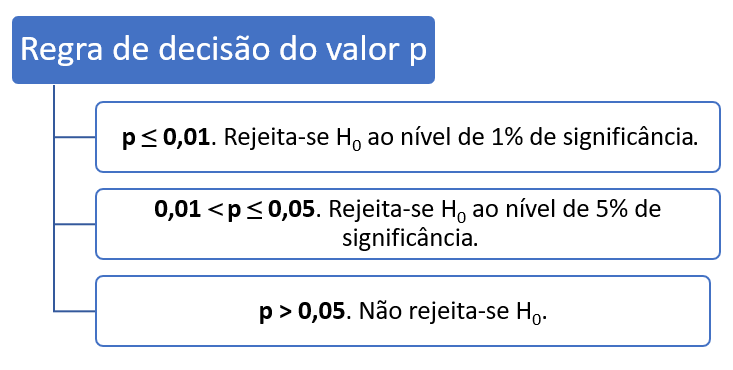
\includegraphics[width=\textwidth]{testehip1} 

}

\caption{Teste de hipóteses}\label{fig:testehip1}
\end{figure}

\begin{Shaded}
\begin{Highlighting}[]
\KeywordTok{shapiro.test}\NormalTok{(horasestudo)}
\end{Highlighting}
\end{Shaded}

\begin{verbatim}

    Shapiro-Wilk normality test

data:  horasestudo
W = 0.98, p-value = 0.9
\end{verbatim}

Como p \(>\) 0,05, não rejeita-se H0 e conclui-se que os dados seguem
uma distribuição normal.

\hypertarget{intervalo-de-confianca-para-uma-proporcao-populacional}{%
\subsection{Intervalo de confiança para uma proporção
populacional}\label{intervalo-de-confianca-para-uma-proporcao-populacional}}

IC (limite inferior \(\leq\) \(\pi\) \(\leq\) limite superior) = (1 -
\(\alpha\))\%

\textbf{Exemplo 2}: (adaptado de
\url{https://www.passeidireto.com/arquivo/3802950/capitulo7---intervalos-de-confianca})
Entre 500 pessoas entrevistas a respeito de suas preferências
eleitorais, 260 mostraram-se favoráveis ao candidato B. Qual é a
proporção amostral dos favoráveis ao candidato B? E a proporção
populacional dos favoráveis?

Sintaxe no software RStudio:

\texttt{prop.test(x,n,conf.level=nível\ de\ confiança)}

Em que:

x = número de sucessos

n= tamanho da amostra

nível de confiança = 0,90 a 0,99

\begin{Shaded}
\begin{Highlighting}[]
\KeywordTok{prop.test}\NormalTok{(}\DecValTok{260}\NormalTok{,}\DecValTok{500}\NormalTok{)}
\end{Highlighting}
\end{Shaded}

\begin{verbatim}

    1-sample proportions test with continuity correction

data:  260 out of 500, null probability 0.5
X-squared = 0.72, df = 1, p-value = 0.4
alternative hypothesis: true p is not equal to 0.5
95 percent confidence interval:
 0.4752 0.5645
sample estimates:
   p 
0.52 
\end{verbatim}

A proporção amostral dos eleitores favoráveis ao candidato B é de 0,52.

IC (0,48 \(\leq\) \(\pi\) \(\leq\) 0,56) = 95\%

Com 95\% de confiança, a proporção populacional dos eleitores favoráveis
ao candidato B está entre 0,48 e 0,56.

Para mudar o nível de confiança para 90\%:

\begin{Shaded}
\begin{Highlighting}[]
\KeywordTok{prop.test}\NormalTok{(}\DecValTok{260}\NormalTok{,}\DecValTok{500}\NormalTok{,}\DataTypeTok{conf.level =} \FloatTok{0.90}\NormalTok{)}
\end{Highlighting}
\end{Shaded}

\begin{verbatim}

    1-sample proportions test with continuity correction

data:  260 out of 500, null probability 0.5
X-squared = 0.72, df = 1, p-value = 0.4
alternative hypothesis: true p is not equal to 0.5
90 percent confidence interval:
 0.4822 0.5575
sample estimates:
   p 
0.52 
\end{verbatim}

IC (0,48 \(\leq\) \(\pi\) \(\leq\) 0,56) = 90\%

Com 90\% de confiança, a proporção populacional dos eleitores favoráveis
ao candidato B está entre 0,48 e 0,56.

Para mudar o nível de confiança para 99\%:

\begin{Shaded}
\begin{Highlighting}[]
\KeywordTok{prop.test}\NormalTok{(}\DecValTok{260}\NormalTok{,}\DecValTok{500}\NormalTok{,}\DataTypeTok{conf.level =} \FloatTok{0.99}\NormalTok{)}
\end{Highlighting}
\end{Shaded}

\begin{verbatim}

    1-sample proportions test with continuity correction

data:  260 out of 500, null probability 0.5
X-squared = 0.72, df = 1, p-value = 0.4
alternative hypothesis: true p is not equal to 0.5
99 percent confidence interval:
 0.4616 0.5779
sample estimates:
   p 
0.52 
\end{verbatim}

IC (0,46 \(\leq\) \(\pi\) \(\leq\) 0,58) = 99\%

Com 99\% de confiança, a proporção populacional dos eleitores favoráveis
ao candidato B está entre 0,46 e 0,58.

\hypertarget{teste-de-hipoteses}{%
\section{Teste de hipóteses}\label{teste-de-hipoteses}}

O teste de hipóteses é uma outra forma de fazer inferência estatística.
Formula-se uma hipótese (H0) para um parâmetro populacional e, partir de
uma amostra dessa população, aceita-se ou rejeita-se esta hipótese.

\textbf{H0}: hipótese nula (sempre tem a condição de igualdade)

\textbf{H1}: hipótese alternativa (tem o sinal de \(\neq\), \(>\) ou
\(<\))

\hypertarget{teste-de-hipoteses-para-uma-media-populacional}{%
\subsection{Teste de hipóteses para uma média
populacional}\label{teste-de-hipoteses-para-uma-media-populacional}}

H0: \(\mu\) \(=\) \ldots{}\ldots{}

H1: \(\mu\) \(\neq\) \ldots{}\ldots{}

H0: \(\mu\) \(=\) \ldots{}\ldots{}.

H1: \(\mu\) \(>\) \ldots{}\ldots{}..

H0: \(\mu\) \(=\) \ldots{}\ldots{}

H1: \(\mu\) \(<\) \ldots{}\ldots{}

No software RStudio, usa-se o `t.test\textbar{} para a realização do
teste de hipóteses para uma média populacional, levando-se em conta o
valor de p-value para aceitar ou rejeitar H0.

De acordo com as hipóteses, temos variações do \texttt{t.test}, conforme
segue:

sintaxe: \texttt{t.test(amostra,\ opções)}

\begin{itemize}
\tightlist
\item
  \textbf{amostra}: Vetor contendo a amostra da qual se quer testar a
  média populacional.
\item
  \textbf{opções}: alternative: string indicando a hipótese alternativa
  desejada. Valores possíveis: \texttt{"two-sided"}, \texttt{"less"} ou
  \texttt{"greater"}.
\item
  \(\mu\): valor indicando o verdadeiro valor da média populacional.
\end{itemize}

\textbf{Exemplo 3}: (adaptado de
\textless{}www.leg.ufpr.br/\textasciitilde{}paulojus/CE002/pratica/praticase8.xml\textgreater{}
) A precipitação pluviométrica mensal numa certa região nos últimos 9
meses foi a seguinte:

30,5 34,1 27,9 35,0 26,9 30,2 28,3 31,7 25,8

Construa um teste de hipóteses para saber se a média da precipitação
pluviométrica mensal é igual a 30,0 mm.

\textbf{H0}: \(\mu\) \(=\) 30 mm

\textbf{H1}: \(\mu\) \(\neq\) 30 mm

\begin{Shaded}
\begin{Highlighting}[]
\NormalTok{chuva=}\KeywordTok{c}\NormalTok{(}\FloatTok{30.5}\NormalTok{,}\FloatTok{34.1}\NormalTok{,}\FloatTok{27.9}\NormalTok{,}\DecValTok{35}\NormalTok{,}\FloatTok{26.9}\NormalTok{,}\FloatTok{30.2}\NormalTok{,}\FloatTok{28.3}\NormalTok{,}\FloatTok{31.7}\NormalTok{,}\FloatTok{25.8}\NormalTok{)}
\NormalTok{chuva}
\end{Highlighting}
\end{Shaded}

\begin{verbatim}
[1] 30.5 34.1 27.9 35.0 26.9 30.2 28.3 31.7 25.8
\end{verbatim}

\begin{Shaded}
\begin{Highlighting}[]
\KeywordTok{t.test}\NormalTok{(chuva,}\DataTypeTok{alt=}\StringTok{"two.sided"}\NormalTok{,}\DataTypeTok{mu=}\DecValTok{30}\NormalTok{)}
\end{Highlighting}
\end{Shaded}

\begin{verbatim}

    One Sample t-test

data:  chuva
t = 0.042, df = 8, p-value = 1
alternative hypothesis: true mean is not equal to 30
95 percent confidence interval:
 27.62 32.47
sample estimates:
mean of x 
    30.04 
\end{verbatim}

Conclusão: Aceita-se H0 e conclui-se que a precipitação pluviométrica é
igual a 30mm.

\textbf{Exemplo 4}: (adaptado de
\url{https://www.passeidireto.com/arquivo/5533375/lista-eststistica-pronta-p-3-prova-com-respostas/3})
Um empresário desconfia que o tempo médio de espera para atendimento de
seus clientes é superior a 20 minutos. Para testar essa hipótese ele
entrevistou 20 pessoas e questionou quanto tempo demorou para ser
atendido. O resultado dessa pesquisa foi o seguinte:

22 20 21 23 22 20 23 22 20 24 21 20 21 24 22 22 23 22 20 24

Teste a hipótese de que o tempo de espera é superior a 20 minutos.

\textbf{H0}: \(\mu\) \(=\) 20 minutos

\textbf{H1}: \(\mu\) \(>\) 20 minutos

\begin{Shaded}
\begin{Highlighting}[]
\NormalTok{tempo=}\KeywordTok{c}\NormalTok{(}\DecValTok{22}\NormalTok{,}\DecValTok{20}\NormalTok{,}\DecValTok{21}\NormalTok{,}\DecValTok{23}\NormalTok{,}\DecValTok{22}\NormalTok{,}\DecValTok{20}\NormalTok{,}\DecValTok{23}\NormalTok{,}\DecValTok{22}\NormalTok{,}\DecValTok{20}\NormalTok{,}\DecValTok{24}\NormalTok{,}\DecValTok{21}\NormalTok{,}\DecValTok{20}\NormalTok{,}\DecValTok{21}\NormalTok{,}\DecValTok{24}\NormalTok{,}\DecValTok{22}\NormalTok{,}\DecValTok{22}\NormalTok{,}\DecValTok{23}\NormalTok{,}\DecValTok{22}\NormalTok{,}\DecValTok{20}\NormalTok{,}\DecValTok{24}\NormalTok{)}
\NormalTok{tempo}
\end{Highlighting}
\end{Shaded}

\begin{verbatim}
 [1] 22 20 21 23 22 20 23 22 20 24 21 20 21 24 22 22 23 22 20 24
\end{verbatim}

\begin{Shaded}
\begin{Highlighting}[]
\KeywordTok{t.test}\NormalTok{(tempo,}\DataTypeTok{alt=}\StringTok{"greater"}\NormalTok{,}\DataTypeTok{mu=}\DecValTok{20}\NormalTok{)}
\end{Highlighting}
\end{Shaded}

\begin{verbatim}

    One Sample t-test

data:  tempo
t = 5.8, df = 19, p-value = 8e-06
alternative hypothesis: true mean is greater than 20
95 percent confidence interval:
 21.26   Inf
sample estimates:
mean of x 
     21.8 
\end{verbatim}

Conclusão: Rejeita-se H0 com nível de significância de 1\% e conclui-se
que o tempo de espera é superior a 20 minutos.

\textbf{Exemplo 5}: (adaptado de
\url{https://docs.ufpr.br/~vayego/pdf_11_2/pratica_04_zoo.pdf}) Os
resíduos industriais jogados nos rios, muitas vezes, absorvem oxigênio,
reduzindo assim o conteúdo do oxigênio necessário à respiração dos
peixes e outras formas de vida aquática. Uma lei estadual exige um
mínimo de 5 p.p.m. (Partes por milhão) de oxigênio dissolvido, a fim de
que o conteúdo de oxigênio seja suficiente para manter a vida aquática.
Seis amostras de água retiradas de um rio, durante a maré baixa,
revelaram os índices (em partes por milhão) de oxigênio dissolvido:

4,9 5,1 4,9 5,5 5,0 4,7

Estes dados são evidência para afirmar que o conteúdo de oxigênio é
menor que 5 partes por milhão?

\textbf{H0}: \(\mu\) \(=\) 5 ppm

\textbf{H1}: \(\mu\) \(<\) 5 ppm

\begin{Shaded}
\begin{Highlighting}[]
\NormalTok{amostras=}\KeywordTok{c}\NormalTok{(}\FloatTok{4.9}\NormalTok{,}\FloatTok{5.1}\NormalTok{,}\FloatTok{4.9}\NormalTok{,}\FloatTok{5.5}\NormalTok{,}\FloatTok{5.0}\NormalTok{,}\FloatTok{4.7}\NormalTok{)}
\KeywordTok{t.test}\NormalTok{(amostras,}\DataTypeTok{alt=}\StringTok{"less"}\NormalTok{,}\DataTypeTok{mu=}\DecValTok{5}\NormalTok{)}
\end{Highlighting}
\end{Shaded}

\begin{verbatim}

    One Sample t-test

data:  amostras
t = 0.15, df = 5, p-value = 0.6
alternative hypothesis: true mean is less than 5
95 percent confidence interval:
 -Inf 5.24
sample estimates:
mean of x 
    5.017 
\end{verbatim}

Conclusão: Aceita-se H0 e conclui-se que o conteúdo de oxigênio é igual
a 5 ppm.

\hypertarget{teste-de-hipoteses-para-uma-proporcao-populacional}{%
\subsection{Teste de hipóteses para uma proporção
populacional}\label{teste-de-hipoteses-para-uma-proporcao-populacional}}

H0: \(\pi\) \(=\) \ldots{}\ldots{}

H1: \(\pi\) \(\neq\) \ldots{}\ldots{}

H0: \(\pi\) \(=\) \ldots{}\ldots{}.

H1: \(\pi\) \(>\) \ldots{}\ldots{}..

H0: \(\pi\) \(=\) \ldots{}\ldots{}

H1: \(\pi\) \(<\) \ldots{}\ldots{}

No software RStudio, usa-se o prop.test para a realização do teste de
hipóteses para uma proporção populacional, levando-se em conta o valor
de p-value para aceitar ou rejeitar H0.

Sintaxe:

\texttt{prop.test(x,n,p=.....,alt=".....")}

em que:

x = número de sucessos;

n= tamanho da amostra;

p = proporção a ser testada;

alt = \texttt{"two.sided"}, \texttt{"greater"} ou \texttt{"less"}.

\textbf{Exemplo 6}: (adaptado de
\url{https://docs.ufpr.br/~soniaisoldi/TP707/Aula8.pdf}) Uma máquina
está regulada quanto produz 3\% de peças defeituosas. Uma amostra
aleatória de 80 peças selecionadas ao acaso apresentou 3 peças
defeituosas. Teste a hipótese de que a máquina está regulada.

\textbf{H0}: \(\pi\) \(=\) 3\%

\textbf{H1}: \(\pi\) \(\neq\) 3\%

\begin{Shaded}
\begin{Highlighting}[]
\KeywordTok{prop.test}\NormalTok{(}\DecValTok{3}\NormalTok{,}\DecValTok{80}\NormalTok{,}\DataTypeTok{p=}\FloatTok{0.03}\NormalTok{,}\DataTypeTok{alt=}\StringTok{"two.sided"}\NormalTok{)}
\end{Highlighting}
\end{Shaded}

\begin{verbatim}
Warning in prop.test(3, 80, p = 0.03, alt = "two.sided"): Chi-squared
approximation may be incorrect
\end{verbatim}

\begin{verbatim}

    1-sample proportions test with continuity correction

data:  3 out of 80, null probability 0.03
X-squared = 0.0043, df = 1, p-value = 0.9
alternative hypothesis: true p is not equal to 0.03
95 percent confidence interval:
 0.009735 0.113171
sample estimates:
     p 
0.0375 
\end{verbatim}

Conclusão: Aceita-se H0 e conclui-se que a máquina produz 3\% de peças
defeituosas, ou seja, a máquina está regulada.

\textbf{Exemplo 7}: (adaptado de
\textless{}www.ebah.com.br/content/ABAAAAdLkAI/metodos-estatistico-und-v-lista-resolvida\textgreater{})
As condições de mortalidade de uma região são tais que a proporção de
nascidos que sobrevivem até 60 anos é de 0,6. Testar essa hipótese se em
1.000 nascimentos amostrados aleatoriamente, verificou-se 530
sobreviventes até 60 anos.

\textbf{H0}: \(\pi\) \(=\) 0,6

\textbf{H1}: \(\pi\) \(\neq\) 0,6

\begin{Shaded}
\begin{Highlighting}[]
\KeywordTok{prop.test}\NormalTok{(}\DecValTok{530}\NormalTok{,}\DecValTok{1000}\NormalTok{,}\DataTypeTok{p=}\FloatTok{0.6}\NormalTok{,}\DataTypeTok{alt=}\StringTok{"two.sided"}\NormalTok{)}
\end{Highlighting}
\end{Shaded}

\begin{verbatim}

    1-sample proportions test with continuity correction

data:  530 out of 1000, null probability 0.6
X-squared = 20, df = 1, p-value = 7e-06
alternative hypothesis: true p is not equal to 0.6
95 percent confidence interval:
 0.4985 0.5613
sample estimates:
   p 
0.53 
\end{verbatim}

Conclusão: Rejeita-se H0 com nível de significância de 1\% e conclui-se
que a proporção de nascidos que sobrevivem até os 60 anos é diferente de
0,6.

\textbf{Exemplo 8}: (adaptado de
\url{https://docs.ufpr.br/~jomarc/intervaloeteste.pdf}) Uma empresa
retira periodicamente amostras aleatórias de 500 peças de sua linha de
produção para análise da qualidade. As peças da amostra são
classificadas como defeituosas ou não, sendo que a política da empresa
exige que o processo produtivo seja revisto se houver evidência de mais
de 1,5\% de peças defeituosas. Na última amostra, foram encontradas nove
peças defeituosas. O processo precisa ser revisto?

\textbf{H0}: \(\pi\) \(=\) 1,5\%

\textbf{H1}: \(\pi\) \(>\) 1,5\%

\begin{Shaded}
\begin{Highlighting}[]
\KeywordTok{prop.test}\NormalTok{(}\DecValTok{9}\NormalTok{,}\DecValTok{500}\NormalTok{,}\DataTypeTok{p=}\FloatTok{0.015}\NormalTok{,}\DataTypeTok{alt=}\StringTok{"greater"}\NormalTok{)}
\end{Highlighting}
\end{Shaded}

\begin{verbatim}

    1-sample proportions test with continuity correction

data:  9 out of 500, null probability 0.015
X-squared = 0.14, df = 1, p-value = 0.4
alternative hypothesis: true p is greater than 0.015
95 percent confidence interval:
 0.009766 1.000000
sample estimates:
    p 
0.018 
\end{verbatim}

Conclusão: Não rejeita H0 e conclui-se que a proporção de peças
defeituosas é igual a 1,5\%, ou seja, o processo não precisa ser
revisto.

\textbf{Exemplo 9}: (adaptado de
\url{https://www.passeidireto.com/arquivo/25297344/aula-19---testes-para-proporcao})
Uma pesquisa conclui que 90\% dos médicos recomendam aspirina a
pacientes que têm filhos. Teste a afirmação contra a alternativa de que
a percentagem é inferior a 90\%, se numa amostra aleatória de 100
médicos, 80 recomendam aspirina.

\textbf{H0}: \(\pi\) \(=\) 90\%

\textbf{H1}: \(\pi\) \(<\) 90\%

\begin{Shaded}
\begin{Highlighting}[]
\KeywordTok{prop.test}\NormalTok{(}\DecValTok{80}\NormalTok{,}\DecValTok{100}\NormalTok{,}\DataTypeTok{p=}\FloatTok{0.90}\NormalTok{,}\DataTypeTok{alt=}\StringTok{"less"}\NormalTok{)}
\end{Highlighting}
\end{Shaded}

\begin{verbatim}

    1-sample proportions test with continuity correction

data:  80 out of 100, null probability 0.9
X-squared = 10, df = 1, p-value = 8e-04
alternative hypothesis: true p is less than 0.9
95 percent confidence interval:
 0.0000 0.8618
sample estimates:
  p 
0.8 
\end{verbatim}

Conclusão: Rejeita-se H0 com nível de significância de 1\% e conclui-se
que a proporção de médicos que recomendam aaspirina é inferior a 90\%.

\hypertarget{teste-de-hipotese-para-duas-medias}{%
\subsection{Teste de hipótese para duas
médias}\label{teste-de-hipotese-para-duas-medias}}

O teste de hipótese para duas médias aplica-se quando se deseja comparar
dois grupos:

\begin{figure}

{\centering 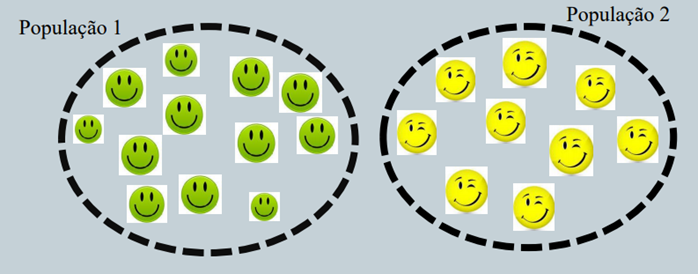
\includegraphics[width=\textwidth]{testehip2} 

}

\caption{Teste de hipótese para dois grupos}\label{fig:testehip2}
\end{figure}

Podemos comparar duas médias de duas amostras dependentes, também
chamadas de pareadas, ou médias de duas amostras independentes.

\hypertarget{teste-de-hipoteses-duas-amostras-dependentes}{%
\subsubsection{Teste de hipóteses duas amostras
dependentes}\label{teste-de-hipoteses-duas-amostras-dependentes}}

\textbf{Exemplo 10}: Foi obtido o peso de seis indivíduos antes e após
um treinamento de exercício físico. Teste a hipótese de que a média
antes do treinamento é diferente da média após o treinamento.

\begin{table}

\caption{\label{tab:unnamed-chunk-107}Amostras dependentes}
\centering
\begin{tabular}[t]{l|r|r|r|r|r|r}
\hline
Indivíduo & A & B & C & D & E & F\\
\hline
Peso antes do treinamento & 99 & 62 & 74 & 59 & 70 & 73\\
\hline
Peso depois do treinamento & 94 & 62 & 66 & 58 & 70 & 76\\
\hline
\end{tabular}
\end{table}

No software RStudio, usa-se o `t.test\textbar{} para a realização do
teste de hipóteses para uma média populacional, levando-se em conta o
valor de p-value para aceitar ou rejeitar H0.

Hipóteses:

\textbf{H0}: média antes \(=\) média depois

\textbf{H1}: média antes \(\neq\) média depois

\begin{Shaded}
\begin{Highlighting}[]
\NormalTok{antes=}\KeywordTok{c}\NormalTok{(}\DecValTok{99}\NormalTok{,}\DecValTok{62}\NormalTok{,}\DecValTok{74}\NormalTok{,}\DecValTok{59}\NormalTok{,}\DecValTok{70}\NormalTok{,}\DecValTok{73}\NormalTok{)}
\NormalTok{depois=}\KeywordTok{c}\NormalTok{(}\DecValTok{94}\NormalTok{,}\DecValTok{62}\NormalTok{,}\DecValTok{66}\NormalTok{,}\DecValTok{58}\NormalTok{,}\DecValTok{70}\NormalTok{,}\DecValTok{76}\NormalTok{)}
\KeywordTok{t.test}\NormalTok{(antes,depois,}\DataTypeTok{paired=}\OtherTok{TRUE}\NormalTok{)}
\end{Highlighting}
\end{Shaded}

\begin{verbatim}

    Paired t-test

data:  antes and depois
t = 1.1, df = 5, p-value = 0.3
alternative hypothesis: true difference in means is not equal to 0
95 percent confidence interval:
 -2.334  6.000
sample estimates:
mean of the differences 
                  1.833 
\end{verbatim}

Conclusão: Não rejeita-se H0 e conclui-se que a média de peso antes do
treinamento é igual à média de peso depois do treinamento.

\textbf{Exemplo 11}: (adaptado de
\textless{}www.inf.ufsc.br/\textasciitilde{}marcelo/testes2.html\textgreater{})
Dez cobaias foram submetidas ao tratamento de engorda com certa ração.
Os pesos em gramas, antes e após o teste são dados a seguir. Podemos
concluir que o uso da ração contribuiu para o aumento do peso médio dos
animais?

\begin{table}

\caption{\label{tab:unnamed-chunk-109}Amostras dependentes - caso 2}
\centering
\begin{tabular}[t]{l|r|r|r|r|r|r|r|r|r|r}
\hline
Cobaia & 1 & 2 & 3 & 4 & 5 & 6 & 7 & 8 & 9 & 10\\
\hline
Antes & 635 & 704 & 662 & 560 & 603 & 745 & 698 & 575 & 633 & 669\\
\hline
Depois & 640 & 712 & 681 & 558 & 610 & 740 & 707 & 585 & 635 & 682\\
\hline
\end{tabular}
\end{table}

\textbf{H0}: média antes \(=\) média depois

\textbf{H1}: média antes \(\neq\) média depois

\begin{Shaded}
\begin{Highlighting}[]
\NormalTok{cobaiaantes=}\KeywordTok{c}\NormalTok{(}\DecValTok{635}\NormalTok{,}\DecValTok{704}\NormalTok{,}\DecValTok{662}\NormalTok{,}\DecValTok{560}\NormalTok{,}\DecValTok{603}\NormalTok{,}\DecValTok{745}\NormalTok{,}\DecValTok{698}\NormalTok{,}\DecValTok{575}\NormalTok{,}\DecValTok{633}\NormalTok{,}\DecValTok{669}\NormalTok{)}
\NormalTok{cobaiadepois=}\KeywordTok{c}\NormalTok{(}\DecValTok{640}\NormalTok{,}\DecValTok{712}\NormalTok{,}\DecValTok{681}\NormalTok{,}\DecValTok{558}\NormalTok{,}\DecValTok{610}\NormalTok{,}\DecValTok{740}\NormalTok{,}\DecValTok{707}\NormalTok{,}\DecValTok{585}\NormalTok{,}\DecValTok{635}\NormalTok{,}\DecValTok{682}\NormalTok{)}
\KeywordTok{t.test}\NormalTok{(cobaiaantes,cobaiadepois,}\DataTypeTok{paired=}\OtherTok{TRUE}\NormalTok{)}
\end{Highlighting}
\end{Shaded}

\begin{verbatim}

    Paired t-test

data:  cobaiaantes and cobaiadepois
t = -3, df = 9, p-value = 0.02
alternative hypothesis: true difference in means is not equal to 0
95 percent confidence interval:
 -11.638  -1.562
sample estimates:
mean of the differences 
                   -6.6 
\end{verbatim}

Conclusão: Rejeita-se H0 com nível de significância de 5\% e conclui-se
que a média antes da engorda é diferente da média depois da engorda.

\hypertarget{teste-de-hipoteses-duas-amostras-independentes}{%
\subsubsection{Teste de hipóteses duas amostras
independentes}\label{teste-de-hipoteses-duas-amostras-independentes}}

Primeiramente precisamos saber se existe homogeneidade de variâncias
populacionais, a qual poderá ser verificada por meio de um teste de
homogeneidade de variâncias utilizando os dados das duas amostras.

\hypertarget{teste-para-verificar-homogeneidade-de-variancias}{%
\paragraph{Teste para verificar homogeneidade de
variâncias}\label{teste-para-verificar-homogeneidade-de-variancias}}

\textbf{Exemplo 12}: (adaptado de
\url{https://www.ime.unicamp.br/~hildete/Aula_p12.pdf}) Dois tipos
diferentes de tecido devem ser comparados. Uma máquina de testes pode
comparar duas amostras ao mesmo tempo. O peso (em miligramas) para sete
experimentos foram:

\begin{table}

\caption{\label{tab:unnamed-chunk-111}Comparação de dois tipos diferentes de tecidos}
\centering
\begin{tabular}[t]{l|l|l|l|l|l|l|l}
\hline
Tecido A & 36 & 26 & 31 & 38 & 28 & 20 & 37\\
\hline
Tecido B & 39 & 27 & 35 & 42 & 31 & 39 & 22\\
\hline
\end{tabular}
\end{table}

Teste se um tecido é mais pesado que o outro.

\textbf{H0}: as variâncias são homogêneas

\textbf{H1}: as variâncias são heterogêneas

\begin{Shaded}
\begin{Highlighting}[]
\NormalTok{tecidoa=}\KeywordTok{c}\NormalTok{(}\DecValTok{36}\NormalTok{,}\DecValTok{26}\NormalTok{,}\DecValTok{31}\NormalTok{,}\DecValTok{38}\NormalTok{,}\DecValTok{28}\NormalTok{,}\DecValTok{20}\NormalTok{,}\DecValTok{37}\NormalTok{)}
\NormalTok{tecidob=}\KeywordTok{c}\NormalTok{(}\DecValTok{39}\NormalTok{,}\DecValTok{27}\NormalTok{,}\DecValTok{35}\NormalTok{,}\DecValTok{42}\NormalTok{,}\DecValTok{31}\NormalTok{,}\DecValTok{39}\NormalTok{,}\DecValTok{22}\NormalTok{)}
\KeywordTok{var.test}\NormalTok{(tecidoa,tecidob)}
\end{Highlighting}
\end{Shaded}

\begin{verbatim}

    F test to compare two variances

data:  tecidoa and tecidob
F = 0.84, num df = 6, denom df = 6, p-value = 0.8
alternative hypothesis: true ratio of variances is not equal to 1
95 percent confidence interval:
 0.1441 4.8823
sample estimates:
ratio of variances 
            0.8389 
\end{verbatim}

Conclusão: Não rejeita-se H0 e conclui-se que as variâncias são
homogêneas.

Agora podemos realizar o teste de comparação de duas amostras
independentes.

\textbf{H0}: média tecido A \(=\) média tecido B

\textbf{H1}: média tecido A \(\neq\) média tecido B

\begin{Shaded}
\begin{Highlighting}[]
\KeywordTok{t.test}\NormalTok{(tecidoa, tecidob, }\DataTypeTok{var.equal =} \OtherTok{TRUE}\NormalTok{, }\DataTypeTok{paired=}\OtherTok{FALSE}\NormalTok{)}
\end{Highlighting}
\end{Shaded}

\begin{verbatim}

    Two Sample t-test

data:  tecidoa and tecidob
t = -0.73, df = 12, p-value = 0.5
alternative hypothesis: true difference in means is not equal to 0
95 percent confidence interval:
 -10.815   5.386
sample estimates:
mean of x mean of y 
    30.86     33.57 
\end{verbatim}

Conclusão: Não rejeita-se H0 e conclui-se que a média de peso do tecido
A é igual à média de peso do tecido B.

\hypertarget{qui}{%
\chapter{Teste de Qui-Quadrado}\label{qui}}

\hypertarget{reg}{%
\chapter{Modelos de Regressão}\label{reg}}

\hypertarget{rmark}{%
\chapter{RMarkdown}\label{rmark}}

\hypertarget{referencias}{%
\chapter*{Referências}\label{referencias}}
\addcontentsline{toc}{chapter}{Referências}

\printbibliography


\end{document}
